\documentclass[twoside]{book}

% Packages required by doxygen
\usepackage{calc}
\usepackage{doxygen}
\usepackage{graphicx}
\usepackage[utf8]{inputenc}
\usepackage{makeidx}
\usepackage{multicol}
\usepackage{multirow}
\usepackage{textcomp}
\usepackage[table]{xcolor}

% Font selection
\usepackage[T1]{fontenc}
\usepackage{mathptmx}
\usepackage[scaled=.90]{helvet}
\usepackage{courier}
\usepackage{amssymb}
\usepackage{sectsty}
\renewcommand{\familydefault}{\sfdefault}
\allsectionsfont{%
  \fontseries{bc}\selectfont%
  \color{darkgray}%
}
\renewcommand{\DoxyLabelFont}{%
  \fontseries{bc}\selectfont%
  \color{darkgray}%
}

% Page & text layout
\usepackage{geometry}
\geometry{%
  a4paper,%
  top=2.5cm,%
  bottom=2.5cm,%
  left=2.5cm,%
  right=2.5cm%
}
\tolerance=750
\hfuzz=15pt
\hbadness=750
\setlength{\emergencystretch}{15pt}
\setlength{\parindent}{0cm}
\setlength{\parskip}{0.2cm}
\makeatletter
\renewcommand{\paragraph}{%
  \@startsection{paragraph}{4}{0ex}{-1.0ex}{1.0ex}{%
    \normalfont\normalsize\bfseries\SS@parafont%
  }%
}
\renewcommand{\subparagraph}{%
  \@startsection{subparagraph}{5}{0ex}{-1.0ex}{1.0ex}{%
    \normalfont\normalsize\bfseries\SS@subparafont%
  }%
}
\makeatother

% Headers & footers
\usepackage{fancyhdr}
\pagestyle{fancyplain}
\fancyhead[LE]{\fancyplain{}{\bfseries\thepage}}
\fancyhead[CE]{\fancyplain{}{}}
\fancyhead[RE]{\fancyplain{}{\bfseries\leftmark}}
\fancyhead[LO]{\fancyplain{}{\bfseries\rightmark}}
\fancyhead[CO]{\fancyplain{}{}}
\fancyhead[RO]{\fancyplain{}{\bfseries\thepage}}
\fancyfoot[LE]{\fancyplain{}{}}
\fancyfoot[CE]{\fancyplain{}{}}
\fancyfoot[RE]{\fancyplain{}{\bfseries\scriptsize Generated on Mon Dec 16 2013 00\-:21\-:19 for Bombás játék by Doxygen }}
\fancyfoot[LO]{\fancyplain{}{\bfseries\scriptsize Generated on Mon Dec 16 2013 00\-:21\-:19 for Bombás játék by Doxygen }}
\fancyfoot[CO]{\fancyplain{}{}}
\fancyfoot[RO]{\fancyplain{}{}}
\renewcommand{\footrulewidth}{0.4pt}
\renewcommand{\chaptermark}[1]{%
  \markboth{#1}{}%
}
\renewcommand{\sectionmark}[1]{%
  \markright{\thesection\ #1}%
}

% Indices & bibliography
\usepackage{natbib}
\usepackage[titles]{tocloft}
\setcounter{tocdepth}{3}
\setcounter{secnumdepth}{5}
\makeindex

% Hyperlinks (required, but should be loaded last)
\usepackage{ifpdf}
\ifpdf
  \usepackage[pdftex,pagebackref=true]{hyperref}
\else
  \usepackage[ps2pdf,pagebackref=true]{hyperref}
\fi
\hypersetup{%
  colorlinks=true,%
  linkcolor=blue,%
  citecolor=blue,%
  unicode%
}

% Custom commands
\newcommand{\clearemptydoublepage}{%
  \newpage{\pagestyle{empty}\cleardoublepage}%
}


%===== C O N T E N T S =====

\begin{document}

% Titlepage & ToC
\hypersetup{pageanchor=false}
\pagenumbering{roman}
\begin{titlepage}
\vspace*{7cm}
\begin{center}%
{\Large Bombás játék }\\
\vspace*{1cm}
{\large Generated by Doxygen 1.8.5}\\
\vspace*{0.5cm}
{\small Mon Dec 16 2013 00:21:19}\\
\end{center}
\end{titlepage}
\clearemptydoublepage
\tableofcontents
\clearemptydoublepage
\pagenumbering{arabic}
\hypersetup{pageanchor=true}

%--- Begin generated contents ---
\chapter{Hierarchical Index}
\section{Class Hierarchy}
This inheritance list is sorted roughly, but not completely, alphabetically\-:\begin{DoxyCompactList}
\item \contentsline{section}{Animation}{\pageref{class_animation}}{}
\item \contentsline{section}{Anim\-File}{\pageref{class_anim_file}}{}
\item \contentsline{section}{Bomb}{\pageref{class_bomb}}{}
\item \contentsline{section}{Client}{\pageref{class_client}}{}
\item \contentsline{section}{Config}{\pageref{class_config}}{}
\item \contentsline{section}{Control}{\pageref{class_control}}{}
\item \contentsline{section}{Flame}{\pageref{class_flame}}{}
\item \contentsline{section}{Frame}{\pageref{struct_frame}}{}
\item \contentsline{section}{Game}{\pageref{class_game}}{}
\item \contentsline{section}{Game\-Config}{\pageref{class_game_config}}{}
\item \contentsline{section}{Game\-Manager}{\pageref{class_game_manager}}{}
\item \contentsline{section}{Game\-Table}{\pageref{class_game_table}}{}
\item \contentsline{section}{Goods}{\pageref{class_goods}}{}
\item \contentsline{section}{Ground}{\pageref{class_ground}}{}
\item \contentsline{section}{Input}{\pageref{class_input}}{}
\item \contentsline{section}{Logger}{\pageref{class_logger}}{}
\item \contentsline{section}{Matrix$<$ T $>$}{\pageref{class_matrix}}{}
\item \contentsline{section}{Matrix$<$ Ground $>$}{\pageref{class_matrix}}{}
\item \contentsline{section}{Matrix$<$ Utf8 $>$}{\pageref{class_matrix}}{}
\item \contentsline{section}{Menu}{\pageref{class_menu}}{}
\item \contentsline{section}{Menu\-Item}{\pageref{class_menu_item}}{}
\item \contentsline{section}{Monster}{\pageref{class_monster}}{}
\item \contentsline{section}{Msgbox}{\pageref{class_msgbox}}{}
\item \contentsline{section}{Network}{\pageref{class_network}}{}
\item \contentsline{section}{Network\-Event}{\pageref{class_network_event}}{}
\item \contentsline{section}{Object}{\pageref{class_object}}{}
\begin{DoxyCompactList}
\item \contentsline{section}{Anim\-Object}{\pageref{class_anim_object}}{}
\item \contentsline{section}{Multi}{\pageref{class_multi}}{}
\item \contentsline{section}{Sprite}{\pageref{class_sprite}}{}
\item \contentsline{section}{Text}{\pageref{class_text}}{}
\end{DoxyCompactList}
\item \contentsline{section}{Player}{\pageref{class_player}}{}
\item \contentsline{section}{Point$<$ T $>$}{\pageref{class_point}}{}
\item \contentsline{section}{Point$<$ float $>$}{\pageref{class_point}}{}
\item \contentsline{section}{Point$<$ int $>$}{\pageref{class_point}}{}
\item \contentsline{section}{Rect}{\pageref{struct_rect}}{}
\item \contentsline{section}{Score\-Board}{\pageref{class_score_board}}{}
\item \contentsline{section}{Select}{\pageref{class_select}}{}
\item \contentsline{section}{Server}{\pageref{class_server}}{}
\item \contentsline{section}{Text\-Input}{\pageref{class_text_input}}{}
\item \contentsline{section}{Translate}{\pageref{class_translate}}{}
\item \contentsline{section}{Utf8}{\pageref{class_utf8}}{}
\item \contentsline{section}{View}{\pageref{class_view}}{}
\end{DoxyCompactList}

\chapter{Class Index}
\section{Class List}
Here are the classes, structs, unions and interfaces with brief descriptions\-:\begin{DoxyCompactList}
\item\contentsline{section}{\hyperlink{class_animation}{Animation} }{\pageref{class_animation}}{}
\item\contentsline{section}{\hyperlink{class_anim_file}{Anim\-File} }{\pageref{class_anim_file}}{}
\item\contentsline{section}{\hyperlink{class_anim_object}{Anim\-Object} }{\pageref{class_anim_object}}{}
\item\contentsline{section}{\hyperlink{class_bomb}{Bomb} }{\pageref{class_bomb}}{}
\item\contentsline{section}{\hyperlink{class_client}{Client} }{\pageref{class_client}}{}
\item\contentsline{section}{\hyperlink{class_config}{Config} }{\pageref{class_config}}{}
\item\contentsline{section}{\hyperlink{class_control}{Control} }{\pageref{class_control}}{}
\item\contentsline{section}{\hyperlink{class_flame}{Flame} }{\pageref{class_flame}}{}
\item\contentsline{section}{\hyperlink{struct_frame}{Frame} }{\pageref{struct_frame}}{}
\item\contentsline{section}{\hyperlink{class_game}{Game} }{\pageref{class_game}}{}
\item\contentsline{section}{\hyperlink{class_game_config}{Game\-Config} }{\pageref{class_game_config}}{}
\item\contentsline{section}{\hyperlink{class_game_manager}{Game\-Manager} }{\pageref{class_game_manager}}{}
\item\contentsline{section}{\hyperlink{class_game_table}{Game\-Table} }{\pageref{class_game_table}}{}
\item\contentsline{section}{\hyperlink{class_goods}{Goods} }{\pageref{class_goods}}{}
\item\contentsline{section}{\hyperlink{class_ground}{Ground} }{\pageref{class_ground}}{}
\item\contentsline{section}{\hyperlink{class_input}{Input} }{\pageref{class_input}}{}
\item\contentsline{section}{\hyperlink{class_logger}{Logger} }{\pageref{class_logger}}{}
\item\contentsline{section}{\hyperlink{class_matrix}{Matrix$<$ T $>$} }{\pageref{class_matrix}}{}
\item\contentsline{section}{\hyperlink{class_menu}{Menu} }{\pageref{class_menu}}{}
\item\contentsline{section}{\hyperlink{class_menu_item}{Menu\-Item} }{\pageref{class_menu_item}}{}
\item\contentsline{section}{\hyperlink{class_monster}{Monster} }{\pageref{class_monster}}{}
\item\contentsline{section}{\hyperlink{class_msgbox}{Msgbox} }{\pageref{class_msgbox}}{}
\item\contentsline{section}{\hyperlink{class_multi}{Multi} }{\pageref{class_multi}}{}
\item\contentsline{section}{\hyperlink{class_network}{Network} }{\pageref{class_network}}{}
\item\contentsline{section}{\hyperlink{class_network_event}{Network\-Event} }{\pageref{class_network_event}}{}
\item\contentsline{section}{\hyperlink{class_object}{Object} }{\pageref{class_object}}{}
\item\contentsline{section}{\hyperlink{class_player}{Player} }{\pageref{class_player}}{}
\item\contentsline{section}{\hyperlink{class_point}{Point$<$ T $>$} }{\pageref{class_point}}{}
\item\contentsline{section}{\hyperlink{struct_rect}{Rect} }{\pageref{struct_rect}}{}
\item\contentsline{section}{\hyperlink{class_score_board}{Score\-Board} }{\pageref{class_score_board}}{}
\item\contentsline{section}{\hyperlink{class_select}{Select} }{\pageref{class_select}}{}
\item\contentsline{section}{\hyperlink{class_server}{Server} }{\pageref{class_server}}{}
\item\contentsline{section}{\hyperlink{class_sprite}{Sprite} }{\pageref{class_sprite}}{}
\item\contentsline{section}{\hyperlink{class_text}{Text} }{\pageref{class_text}}{}
\item\contentsline{section}{\hyperlink{class_text_input}{Text\-Input} }{\pageref{class_text_input}}{}
\item\contentsline{section}{\hyperlink{class_translate}{Translate} }{\pageref{class_translate}}{}
\item\contentsline{section}{\hyperlink{class_utf8}{Utf8} }{\pageref{class_utf8}}{}
\item\contentsline{section}{\hyperlink{class_view}{View} }{\pageref{class_view}}{}
\end{DoxyCompactList}

\chapter{Class Documentation}
\hypertarget{class_animation}{\section{Animation Class Reference}
\label{class_animation}\index{Animation@{Animation}}
}


{\ttfamily \#include $<$animation.\-h$>$}

\subsection*{Public Member Functions}
\begin{DoxyCompactItemize}
\item 
\hyperlink{class_animation_a83f0a16cef7117f187ad596de38dd9d6}{Animation} ()
\item 
\hyperlink{class_animation_a97aee78e26558779ceaf1e9fe246720c}{Animation} (\hyperlink{struct_rect}{Rect} irect, T\-I\-M\-E istart, \hyperlink{class_anim_file}{Anim\-File} $\ast$ianim, std\-::string iparam=\char`\"{}\char`\"{})
\item 
std\-::string \hyperlink{class_animation_a1472a0972103d62a94f493f75ad91fa6}{draw} (T\-I\-M\-E time)
\item 
\hyperlink{struct_rect}{Rect} \hyperlink{class_animation_a62aeb060f1cc2b6cc012ca4461a4ff24}{get\-Rect} ()
\end{DoxyCompactItemize}


\subsection{Detailed Description}
Static animation 

\subsection{Constructor \& Destructor Documentation}
\hypertarget{class_animation_a83f0a16cef7117f187ad596de38dd9d6}{\index{Animation@{Animation}!Animation@{Animation}}
\index{Animation@{Animation}!Animation@{Animation}}
\subsubsection[{Animation}]{\setlength{\rightskip}{0pt plus 5cm}Animation\-::\-Animation (
\begin{DoxyParamCaption}
{}
\end{DoxyParamCaption}
)\hspace{0.3cm}{\ttfamily [inline]}}}\label{class_animation_a83f0a16cef7117f187ad596de38dd9d6}
Default constructor \hypertarget{class_animation_a97aee78e26558779ceaf1e9fe246720c}{\index{Animation@{Animation}!Animation@{Animation}}
\index{Animation@{Animation}!Animation@{Animation}}
\subsubsection[{Animation}]{\setlength{\rightskip}{0pt plus 5cm}Animation\-::\-Animation (
\begin{DoxyParamCaption}
\item[{{\bf Rect}}]{irect, }
\item[{T\-I\-M\-E}]{istart, }
\item[{{\bf Anim\-File} $\ast$}]{ianim, }
\item[{std\-::string}]{iparam = {\ttfamily \char`\"{}\char`\"{}}}
\end{DoxyParamCaption}
)\hspace{0.3cm}{\ttfamily [inline]}}}\label{class_animation_a97aee78e26558779ceaf1e9fe246720c}
Constructor 
\begin{DoxyParams}{Parameters}
{\em irect} & rectangle where the animation will be shown \\
\hline
{\em istart} & start time of animation \\
\hline
{\em ianim} & previously loaded animation file \\
\hline
{\em iparam} & drawing parameters \\
\hline
\end{DoxyParams}


\subsection{Member Function Documentation}
\hypertarget{class_animation_a1472a0972103d62a94f493f75ad91fa6}{\index{Animation@{Animation}!draw@{draw}}
\index{draw@{draw}!Animation@{Animation}}
\subsubsection[{draw}]{\setlength{\rightskip}{0pt plus 5cm}std\-::string Animation\-::draw (
\begin{DoxyParamCaption}
\item[{T\-I\-M\-E}]{time}
\end{DoxyParamCaption}
)\hspace{0.3cm}{\ttfamily [inline]}}}\label{class_animation_a1472a0972103d62a94f493f75ad91fa6}
Draw animation frame regarding time 
\begin{DoxyParams}{Parameters}
{\em time} & current frame time \\
\hline
\end{DoxyParams}
\begin{DoxyReturn}{Returns}
graphic string 
\end{DoxyReturn}
\hypertarget{class_animation_a62aeb060f1cc2b6cc012ca4461a4ff24}{\index{Animation@{Animation}!get\-Rect@{get\-Rect}}
\index{get\-Rect@{get\-Rect}!Animation@{Animation}}
\subsubsection[{get\-Rect}]{\setlength{\rightskip}{0pt plus 5cm}{\bf Rect} Animation\-::get\-Rect (
\begin{DoxyParamCaption}
{}
\end{DoxyParamCaption}
)\hspace{0.3cm}{\ttfamily [inline]}}}\label{class_animation_a62aeb060f1cc2b6cc012ca4461a4ff24}
Rectangle where animation is drawn 

The documentation for this class was generated from the following file\-:\begin{DoxyCompactItemize}
\item 
view/animation.\-h\end{DoxyCompactItemize}

\hypertarget{class_anim_file}{\section{Anim\-File Class Reference}
\label{class_anim_file}\index{Anim\-File@{Anim\-File}}
}


{\ttfamily \#include $<$animfile.\-h$>$}

\subsection*{Public Member Functions}
\begin{DoxyCompactItemize}
\item 
\hyperlink{class_anim_file_ab0276fb61fd8950aed68044a807a00ef}{Anim\-File} ()
\item 
\hyperlink{class_anim_file_aae98d30636cf9343e068957f6ea27b7a}{Anim\-File} (std\-::string filename)
\item 
std\-::string \hyperlink{class_anim_file_a1f05adedf06719b4c41896b02c08fadd}{frame} (T\-I\-M\-E time)
\end{DoxyCompactItemize}


\subsection{Detailed Description}
Descriptor of a static animation 

\subsection{Constructor \& Destructor Documentation}
\hypertarget{class_anim_file_ab0276fb61fd8950aed68044a807a00ef}{\index{Anim\-File@{Anim\-File}!Anim\-File@{Anim\-File}}
\index{Anim\-File@{Anim\-File}!AnimFile@{Anim\-File}}
\subsubsection[{Anim\-File}]{\setlength{\rightskip}{0pt plus 5cm}Anim\-File\-::\-Anim\-File (
\begin{DoxyParamCaption}
{}
\end{DoxyParamCaption}
)\hspace{0.3cm}{\ttfamily [inline]}}}\label{class_anim_file_ab0276fb61fd8950aed68044a807a00ef}
Default constructor \hypertarget{class_anim_file_aae98d30636cf9343e068957f6ea27b7a}{\index{Anim\-File@{Anim\-File}!Anim\-File@{Anim\-File}}
\index{Anim\-File@{Anim\-File}!AnimFile@{Anim\-File}}
\subsubsection[{Anim\-File}]{\setlength{\rightskip}{0pt plus 5cm}Anim\-File\-::\-Anim\-File (
\begin{DoxyParamCaption}
\item[{std\-::string}]{filename}
\end{DoxyParamCaption}
)}}\label{class_anim_file_aae98d30636cf9343e068957f6ea27b7a}
Constructor, loads animation phases 
\begin{DoxyParams}{Parameters}
{\em filename} & name of animation file (.anm) \\
\hline
\end{DoxyParams}


\subsection{Member Function Documentation}
\hypertarget{class_anim_file_a1f05adedf06719b4c41896b02c08fadd}{\index{Anim\-File@{Anim\-File}!frame@{frame}}
\index{frame@{frame}!AnimFile@{Anim\-File}}
\subsubsection[{frame}]{\setlength{\rightskip}{0pt plus 5cm}std\-::string Anim\-File\-::frame (
\begin{DoxyParamCaption}
\item[{T\-I\-M\-E}]{time}
\end{DoxyParamCaption}
)}}\label{class_anim_file_a1f05adedf06719b4c41896b02c08fadd}
Calculate the current animation phase to show depending on current frame time 
\begin{DoxyParams}{Parameters}
{\em time} & frame time \\
\hline
\end{DoxyParams}
\begin{DoxyReturn}{Returns}
graphic name (full draw path) 
\end{DoxyReturn}


The documentation for this class was generated from the following files\-:\begin{DoxyCompactItemize}
\item 
view/animfile.\-h\item 
view/animfile.\-cpp\end{DoxyCompactItemize}

\hypertarget{class_anim_object}{\section{Anim\-Object Class Reference}
\label{class_anim_object}\index{Anim\-Object@{Anim\-Object}}
}


{\ttfamily \#include $<$animobject.\-h$>$}

Inheritance diagram for Anim\-Object\-:\begin{figure}[H]
\begin{center}
\leavevmode
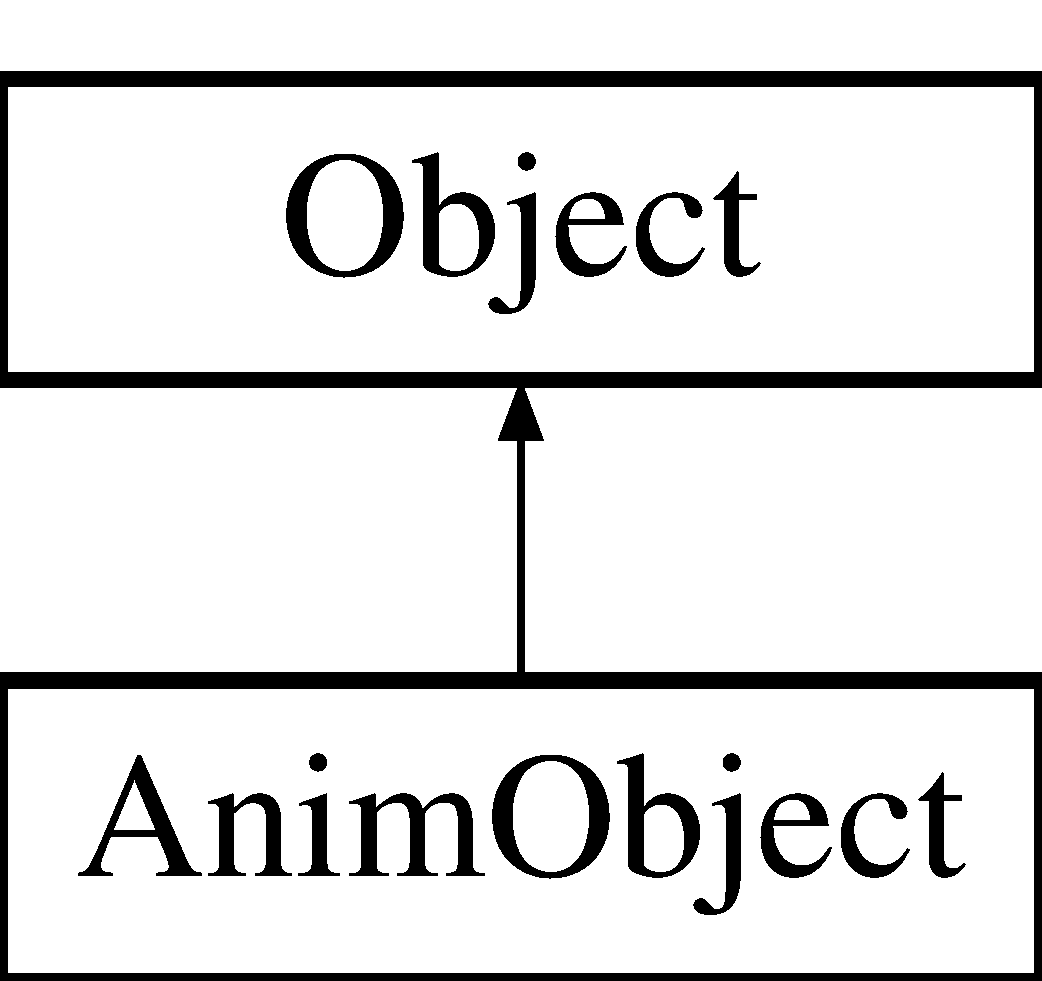
\includegraphics[height=2.000000cm]{class_anim_object}
\end{center}
\end{figure}
\subsection*{Public Member Functions}
\begin{DoxyCompactItemize}
\item 
\hyperlink{class_anim_object_a05d32294cceb9b869d5b4088c430f08b}{Anim\-Object} ()
\item 
\hyperlink{class_anim_object_a6f0092d3c69a4b3af920dd68eab73449}{Anim\-Object} (std\-::deque$<$ \hyperlink{class_animation}{Animation} $>$ $\ast$ianim, std\-::map$<$ std\-::string, \hyperlink{class_anim_file}{Anim\-File} $>$ $\ast$ianims, std\-::string iname, T\-I\-M\-E $\ast$inow)
\item 
void \hyperlink{class_anim_object_a93eda4562497de04bf7db6407d74e5aa}{draw} (float x, float y, float w, float h, std\-::string param=\char`\"{}\char`\"{})
\end{DoxyCompactItemize}


\subsection{Detailed Description}
\hyperlink{class_animation}{Animation} to use in draw 

\subsection{Constructor \& Destructor Documentation}
\hypertarget{class_anim_object_a05d32294cceb9b869d5b4088c430f08b}{\index{Anim\-Object@{Anim\-Object}!Anim\-Object@{Anim\-Object}}
\index{Anim\-Object@{Anim\-Object}!AnimObject@{Anim\-Object}}
\subsubsection[{Anim\-Object}]{\setlength{\rightskip}{0pt plus 5cm}Anim\-Object\-::\-Anim\-Object (
\begin{DoxyParamCaption}
{}
\end{DoxyParamCaption}
)\hspace{0.3cm}{\ttfamily [inline]}}}\label{class_anim_object_a05d32294cceb9b869d5b4088c430f08b}
Default constructor \hypertarget{class_anim_object_a6f0092d3c69a4b3af920dd68eab73449}{\index{Anim\-Object@{Anim\-Object}!Anim\-Object@{Anim\-Object}}
\index{Anim\-Object@{Anim\-Object}!AnimObject@{Anim\-Object}}
\subsubsection[{Anim\-Object}]{\setlength{\rightskip}{0pt plus 5cm}Anim\-Object\-::\-Anim\-Object (
\begin{DoxyParamCaption}
\item[{std\-::deque$<$ {\bf Animation} $>$ $\ast$}]{ianim, }
\item[{std\-::map$<$ std\-::string, {\bf Anim\-File} $>$ $\ast$}]{ianims, }
\item[{std\-::string}]{iname, }
\item[{T\-I\-M\-E $\ast$}]{inow}
\end{DoxyParamCaption}
)\hspace{0.3cm}{\ttfamily [inline]}}}\label{class_anim_object_a6f0092d3c69a4b3af920dd68eab73449}
Constructor 
\begin{DoxyParams}{Parameters}
{\em ianim} & deque of animations from view \\
\hline
{\em ianims} & animation files \\
\hline
{\em iname} & name of animation \\
\hline
{\em inow} & pointer to current frame time \\
\hline
\end{DoxyParams}


\subsection{Member Function Documentation}
\hypertarget{class_anim_object_a93eda4562497de04bf7db6407d74e5aa}{\index{Anim\-Object@{Anim\-Object}!draw@{draw}}
\index{draw@{draw}!AnimObject@{Anim\-Object}}
\subsubsection[{draw}]{\setlength{\rightskip}{0pt plus 5cm}void Anim\-Object\-::draw (
\begin{DoxyParamCaption}
\item[{float}]{x, }
\item[{float}]{y, }
\item[{float}]{w, }
\item[{float}]{h, }
\item[{std\-::string}]{param = {\ttfamily \char`\"{}\char`\"{}}}
\end{DoxyParamCaption}
)\hspace{0.3cm}{\ttfamily [inline]}, {\ttfamily [virtual]}}}\label{class_anim_object_a93eda4562497de04bf7db6407d74e5aa}
Draw animation 
\begin{DoxyParams}{Parameters}
{\em x} & coordinate \\
\hline
{\em y} & coordinate \\
\hline
{\em w} & width \\
\hline
{\em h} & height \\
\hline
{\em param} & graphic parameter \\
\hline
\end{DoxyParams}


Reimplemented from \hyperlink{class_object_a13b99ec4da0a1c798104560c492c2a7e}{Object}.



The documentation for this class was generated from the following file\-:\begin{DoxyCompactItemize}
\item 
view/animobject.\-h\end{DoxyCompactItemize}

\hypertarget{class_bomb}{\section{Bomb Class Reference}
\label{class_bomb}\index{Bomb@{Bomb}}
}


{\ttfamily \#include $<$bomb.\-h$>$}

\subsection*{Public Member Functions}
\begin{DoxyCompactItemize}
\item 
\hyperlink{class_bomb_a5805401b6cfbb451cf31ebd4851740cf}{Bomb} ()
\item 
\hyperlink{class_bomb_a03c2cd4e1bfa472de74d5deb29066f11}{Bomb} (T\-I\-M\-E iactivated, \hyperlink{class_point}{Point}$<$ int $>$ ipoint, \hyperlink{class_player}{Player} $\ast$iplayer)
\item 
void \hyperlink{class_bomb_a1e4a85025c5b31a9e1d7e9200e3e4e90}{boom} ()
\item 
bool \hyperlink{class_bomb_a60cd514206385870458e02327143070f}{boom} (T\-I\-M\-E inow)
\item 
std\-::string \hyperlink{class_bomb_a856d0fab5a4c401a8b3e153dd063d604}{state} ()
\item 
int \hyperlink{class_bomb_a3ed5889d36fa63a00162b92b84a7c363}{get\-X} ()
\item 
int \hyperlink{class_bomb_a1c07f26ec95a76bfca5ecf633e7913a8}{get\-Y} ()
\item 
\hyperlink{class_point}{Point}$<$ int $>$ \hyperlink{class_bomb_a9d2af1296b33a4c06b6b36c8aaf4d45e}{get\-Point} ()
\item 
int \hyperlink{class_bomb_acd1ab69615d334bdbe7f43342c8857e4}{get\-Size} ()
\item 
int \hyperlink{class_bomb_ab2646fe8e30483a297481e6ee7aa728f}{get\-Owner} ()
\end{DoxyCompactItemize}


\subsection{Detailed Description}
\hyperlink{class_bomb}{Bomb} on the game table 

\subsection{Constructor \& Destructor Documentation}
\hypertarget{class_bomb_a5805401b6cfbb451cf31ebd4851740cf}{\index{Bomb@{Bomb}!Bomb@{Bomb}}
\index{Bomb@{Bomb}!Bomb@{Bomb}}
\subsubsection[{Bomb}]{\setlength{\rightskip}{0pt plus 5cm}Bomb\-::\-Bomb (
\begin{DoxyParamCaption}
{}
\end{DoxyParamCaption}
)\hspace{0.3cm}{\ttfamily [inline]}}}\label{class_bomb_a5805401b6cfbb451cf31ebd4851740cf}
Default constructor \hypertarget{class_bomb_a03c2cd4e1bfa472de74d5deb29066f11}{\index{Bomb@{Bomb}!Bomb@{Bomb}}
\index{Bomb@{Bomb}!Bomb@{Bomb}}
\subsubsection[{Bomb}]{\setlength{\rightskip}{0pt plus 5cm}Bomb\-::\-Bomb (
\begin{DoxyParamCaption}
\item[{T\-I\-M\-E}]{iactivated, }
\item[{{\bf Point}$<$ int $>$}]{ipoint, }
\item[{{\bf Player} $\ast$}]{iplayer}
\end{DoxyParamCaption}
)\hspace{0.3cm}{\ttfamily [inline]}}}\label{class_bomb_a03c2cd4e1bfa472de74d5deb29066f11}
Constructor 
\begin{DoxyParams}{Parameters}
{\em iactivated} & when should it become ignited \\
\hline
{\em ipoint} & place of bomb \\
\hline
{\em iplayer} & \hyperlink{class_player}{Player} who put it \\
\hline
\end{DoxyParams}


\subsection{Member Function Documentation}
\hypertarget{class_bomb_a1e4a85025c5b31a9e1d7e9200e3e4e90}{\index{Bomb@{Bomb}!boom@{boom}}
\index{boom@{boom}!Bomb@{Bomb}}
\subsubsection[{boom}]{\setlength{\rightskip}{0pt plus 5cm}void Bomb\-::boom (
\begin{DoxyParamCaption}
{}
\end{DoxyParamCaption}
)\hspace{0.3cm}{\ttfamily [inline]}}}\label{class_bomb_a1e4a85025c5b31a9e1d7e9200e3e4e90}
\hyperlink{class_bomb}{Bomb} ignites by another flame, update player's number of bombs \hypertarget{class_bomb_a60cd514206385870458e02327143070f}{\index{Bomb@{Bomb}!boom@{boom}}
\index{boom@{boom}!Bomb@{Bomb}}
\subsubsection[{boom}]{\setlength{\rightskip}{0pt plus 5cm}bool Bomb\-::boom (
\begin{DoxyParamCaption}
\item[{T\-I\-M\-E}]{inow}
\end{DoxyParamCaption}
)\hspace{0.3cm}{\ttfamily [inline]}}}\label{class_bomb_a60cd514206385870458e02327143070f}
\hyperlink{class_bomb}{Bomb} ignites by time 
\begin{DoxyParams}{Parameters}
{\em inow} & current frame time \\
\hline
\end{DoxyParams}
\begin{DoxyReturn}{Returns}
ignites or not 
\end{DoxyReturn}
\hypertarget{class_bomb_ab2646fe8e30483a297481e6ee7aa728f}{\index{Bomb@{Bomb}!get\-Owner@{get\-Owner}}
\index{get\-Owner@{get\-Owner}!Bomb@{Bomb}}
\subsubsection[{get\-Owner}]{\setlength{\rightskip}{0pt plus 5cm}int Bomb\-::get\-Owner (
\begin{DoxyParamCaption}
{}
\end{DoxyParamCaption}
)\hspace{0.3cm}{\ttfamily [inline]}}}\label{class_bomb_ab2646fe8e30483a297481e6ee7aa728f}
Get owner \begin{DoxyReturn}{Returns}
player I\-D 
\end{DoxyReturn}
\hypertarget{class_bomb_a9d2af1296b33a4c06b6b36c8aaf4d45e}{\index{Bomb@{Bomb}!get\-Point@{get\-Point}}
\index{get\-Point@{get\-Point}!Bomb@{Bomb}}
\subsubsection[{get\-Point}]{\setlength{\rightskip}{0pt plus 5cm}{\bf Point}$<$int$>$ Bomb\-::get\-Point (
\begin{DoxyParamCaption}
{}
\end{DoxyParamCaption}
)\hspace{0.3cm}{\ttfamily [inline]}}}\label{class_bomb_a9d2af1296b33a4c06b6b36c8aaf4d45e}
Get place of bomb \hypertarget{class_bomb_acd1ab69615d334bdbe7f43342c8857e4}{\index{Bomb@{Bomb}!get\-Size@{get\-Size}}
\index{get\-Size@{get\-Size}!Bomb@{Bomb}}
\subsubsection[{get\-Size}]{\setlength{\rightskip}{0pt plus 5cm}int Bomb\-::get\-Size (
\begin{DoxyParamCaption}
{}
\end{DoxyParamCaption}
)\hspace{0.3cm}{\ttfamily [inline]}}}\label{class_bomb_acd1ab69615d334bdbe7f43342c8857e4}
Get flame size \hypertarget{class_bomb_a3ed5889d36fa63a00162b92b84a7c363}{\index{Bomb@{Bomb}!get\-X@{get\-X}}
\index{get\-X@{get\-X}!Bomb@{Bomb}}
\subsubsection[{get\-X}]{\setlength{\rightskip}{0pt plus 5cm}int Bomb\-::get\-X (
\begin{DoxyParamCaption}
{}
\end{DoxyParamCaption}
)\hspace{0.3cm}{\ttfamily [inline]}}}\label{class_bomb_a3ed5889d36fa63a00162b92b84a7c363}
Get X coordinate \hypertarget{class_bomb_a1c07f26ec95a76bfca5ecf633e7913a8}{\index{Bomb@{Bomb}!get\-Y@{get\-Y}}
\index{get\-Y@{get\-Y}!Bomb@{Bomb}}
\subsubsection[{get\-Y}]{\setlength{\rightskip}{0pt plus 5cm}int Bomb\-::get\-Y (
\begin{DoxyParamCaption}
{}
\end{DoxyParamCaption}
)\hspace{0.3cm}{\ttfamily [inline]}}}\label{class_bomb_a1c07f26ec95a76bfca5ecf633e7913a8}
Get Y coordinate \hypertarget{class_bomb_a856d0fab5a4c401a8b3e153dd063d604}{\index{Bomb@{Bomb}!state@{state}}
\index{state@{state}!Bomb@{Bomb}}
\subsubsection[{state}]{\setlength{\rightskip}{0pt plus 5cm}std\-::string Bomb\-::state (
\begin{DoxyParamCaption}
{}
\end{DoxyParamCaption}
)\hspace{0.3cm}{\ttfamily [inline]}}}\label{class_bomb_a856d0fab5a4c401a8b3e153dd063d604}
\hyperlink{class_animation}{Animation} state \begin{DoxyReturn}{Returns}
graphic string 
\end{DoxyReturn}


The documentation for this class was generated from the following file\-:\begin{DoxyCompactItemize}
\item 
bomb.\-h\end{DoxyCompactItemize}

\hypertarget{class_client}{\section{Client Class Reference}
\label{class_client}\index{Client@{Client}}
}


{\ttfamily \#include $<$client.\-h$>$}

\subsection*{Public Member Functions}
\begin{DoxyCompactItemize}
\item 
\hyperlink{class_client_a7bfde03c1d803967f143e43f182f12d1}{Client} (std\-::string i\-Server\-Name)
\item 
\hyperlink{class_client_a840e519ca781888cbd54181572ebe3a7}{$\sim$\-Client} ()
\item 
void \hyperlink{class_client_a654ba5473ed09ebec6ab7c08e7a24c62}{main\-Loop} ()
\item 
bool \hyperlink{class_client_a99e1f6991bf2b4621a78ba939646f30f}{send\-Packets} (std\-::vector$<$ \hyperlink{class_network_event}{Network\-Event} $>$ \&packets\-Out)
\item 
std\-::vector$<$ \hyperlink{class_network_event}{Network\-Event} $>$ \& \hyperlink{class_client_a4b95752c68427742a66c792fd5885a5c}{get\-Packets} ()
\item 
bool \hyperlink{class_client_a9bf1bb055b99eae811954f41533a373d}{get\-Success} () const 
\item 
std\-::string \hyperlink{class_client_a056af8a9a28128d017c0b6b280204575}{get\-Host} () const 
\end{DoxyCompactItemize}


\subsection{Detailed Description}
\hyperlink{class_client}{Client} connection and packet handling 

\subsection{Constructor \& Destructor Documentation}
\hypertarget{class_client_a7bfde03c1d803967f143e43f182f12d1}{\index{Client@{Client}!Client@{Client}}
\index{Client@{Client}!Client@{Client}}
\subsubsection[{Client}]{\setlength{\rightskip}{0pt plus 5cm}Client\-::\-Client (
\begin{DoxyParamCaption}
\item[{std\-::string}]{i\-Server\-Name}
\end{DoxyParamCaption}
)}}\label{class_client_a7bfde03c1d803967f143e43f182f12d1}
Constructor 
\begin{DoxyParams}{Parameters}
{\em i\-Server\-Name} & address to connect (can be I\-P or host name) \\
\hline
\end{DoxyParams}
\hypertarget{class_client_a840e519ca781888cbd54181572ebe3a7}{\index{Client@{Client}!$\sim$\-Client@{$\sim$\-Client}}
\index{$\sim$\-Client@{$\sim$\-Client}!Client@{Client}}
\subsubsection[{$\sim$\-Client}]{\setlength{\rightskip}{0pt plus 5cm}Client\-::$\sim$\-Client (
\begin{DoxyParamCaption}
{}
\end{DoxyParamCaption}
)}}\label{class_client_a840e519ca781888cbd54181572ebe3a7}
Desctructor 

\subsection{Member Function Documentation}
\hypertarget{class_client_a056af8a9a28128d017c0b6b280204575}{\index{Client@{Client}!get\-Host@{get\-Host}}
\index{get\-Host@{get\-Host}!Client@{Client}}
\subsubsection[{get\-Host}]{\setlength{\rightskip}{0pt plus 5cm}std\-::string Client\-::get\-Host (
\begin{DoxyParamCaption}
{}
\end{DoxyParamCaption}
) const\hspace{0.3cm}{\ttfamily [inline]}}}\label{class_client_a056af8a9a28128d017c0b6b280204575}
Get the address we connected to \hypertarget{class_client_a4b95752c68427742a66c792fd5885a5c}{\index{Client@{Client}!get\-Packets@{get\-Packets}}
\index{get\-Packets@{get\-Packets}!Client@{Client}}
\subsubsection[{get\-Packets}]{\setlength{\rightskip}{0pt plus 5cm}std\-::vector$<$ {\bf Network\-Event} $>$ \& Client\-::get\-Packets (
\begin{DoxyParamCaption}
{}
\end{DoxyParamCaption}
)}}\label{class_client_a4b95752c68427742a66c792fd5885a5c}
Get packets (after main\-Loop run) \hypertarget{class_client_a9bf1bb055b99eae811954f41533a373d}{\index{Client@{Client}!get\-Success@{get\-Success}}
\index{get\-Success@{get\-Success}!Client@{Client}}
\subsubsection[{get\-Success}]{\setlength{\rightskip}{0pt plus 5cm}bool Client\-::get\-Success (
\begin{DoxyParamCaption}
{}
\end{DoxyParamCaption}
) const}}\label{class_client_a9bf1bb055b99eae811954f41533a373d}
False if error occured. \hypertarget{class_client_a654ba5473ed09ebec6ab7c08e7a24c62}{\index{Client@{Client}!main\-Loop@{main\-Loop}}
\index{main\-Loop@{main\-Loop}!Client@{Client}}
\subsubsection[{main\-Loop}]{\setlength{\rightskip}{0pt plus 5cm}void Client\-::main\-Loop (
\begin{DoxyParamCaption}
{}
\end{DoxyParamCaption}
)}}\label{class_client_a654ba5473ed09ebec6ab7c08e7a24c62}
Main loop, receive packets \hypertarget{class_client_a99e1f6991bf2b4621a78ba939646f30f}{\index{Client@{Client}!send\-Packets@{send\-Packets}}
\index{send\-Packets@{send\-Packets}!Client@{Client}}
\subsubsection[{send\-Packets}]{\setlength{\rightskip}{0pt plus 5cm}bool Client\-::send\-Packets (
\begin{DoxyParamCaption}
\item[{std\-::vector$<$ {\bf Network\-Event} $>$ \&}]{packets\-Out}
\end{DoxyParamCaption}
)}}\label{class_client_a99e1f6991bf2b4621a78ba939646f30f}
Send packets to server 

The documentation for this class was generated from the following files\-:\begin{DoxyCompactItemize}
\item 
client.\-h\item 
client.\-cpp\end{DoxyCompactItemize}

\hypertarget{class_config}{\section{Config Class Reference}
\label{class_config}\index{Config@{Config}}
}


{\ttfamily \#include $<$config.\-h$>$}

\subsection*{Public Member Functions}
\begin{DoxyCompactItemize}
\item 
\hyperlink{class_config_abd0c571c116924871e30444b192b792a}{Config} ()
\end{DoxyCompactItemize}
\subsection*{Static Public Member Functions}
\begin{DoxyCompactItemize}
\item 
static \hyperlink{class_config}{Config} \& \hyperlink{class_config_a52ae1e3685e26ba3689691b627d33647}{get\-Instance} ()
\end{DoxyCompactItemize}
\subsection*{Public Attributes}
\begin{DoxyCompactItemize}
\item 
int \hyperlink{class_config_a2660688203b9170918c7e2e8e5b54ed4}{C\-F\-G\-\_\-\-F\-L\-A\-M\-E\-T\-I\-M\-E}
\item 
int \hyperlink{class_config_a0574d1159f4788df4ba510d1d3e83498}{C\-F\-G\-\_\-\-B\-O\-M\-B\-T\-I\-M\-E}
\item 
float \hyperlink{class_config_a8f2b0ec592b0bda65e2133e21fe46979}{C\-F\-G\-\_\-\-D\-E\-F\-A\-U\-L\-T\-\_\-\-S\-P\-E\-E\-D}
\item 
float \hyperlink{class_config_a1e059aee7b0dccef0baeae3ac1e51ff8}{C\-F\-G\-\_\-\-S\-L\-O\-W\-\_\-\-S\-P\-E\-E\-D}
\item 
float \hyperlink{class_config_a2e8f4b387f08e51b6bfc9c27905beb60}{C\-F\-G\-\_\-\-F\-A\-S\-T\-\_\-\-S\-P\-E\-E\-D}
\item 
int \hyperlink{class_config_a27f5415363ce485450a5e565fc07eedf}{C\-F\-G\-\_\-\-V\-I\-R\-U\-S\-T\-I\-M\-E}
\item 
int \hyperlink{class_config_a4dca8b903aa44d2eeac1360b3bd8abe3}{C\-F\-G\-\_\-\-R\-E\-S\-P\-A\-W\-N\-\_\-\-P\-L\-A\-Y\-E\-R}
\item 
int \hyperlink{class_config_a68f25bf53407aa4d78dbf20810084c21}{C\-F\-G\-\_\-\-R\-E\-S\-P\-A\-W\-N\-\_\-\-M\-O\-N\-S\-T\-E\-R}
\item 
int \hyperlink{class_config_ad7096d8320756b47101410a630072959}{C\-F\-G\-\_\-\-R\-E\-S\-P\-A\-W\-N\-\_\-\-M\-O\-N\-S\-T\-E\-R\-\_\-\-I\-N\-T\-E\-R\-V\-A\-L}
\item 
int \hyperlink{class_config_aa9c1a6477d3af67f0d9af85abe1ab399}{C\-F\-G\-\_\-\-W\-A\-I\-T\-\_\-\-R\-O\-U\-N\-D}
\item 
int \hyperlink{class_config_a4d8faf4496d7fad5ce922354581e7c2b}{C\-F\-G\-\_\-\-S\-H\-O\-W\-\_\-\-S\-C\-O\-R\-E\-B\-O\-A\-R\-D}
\item 
int \hyperlink{class_config_aba9d64248625f53dee1028d3e4bf687d}{C\-F\-G\-\_\-\-I\-M\-M\-O\-R\-T\-A\-L}
\item 
int \hyperlink{class_config_a254ff81fc5ea5548eebb2183b2735b03}{C\-F\-G\-\_\-\-W\-A\-L\-L\-S\-\_\-\-B\-U\-I\-L\-D\-\_\-\-P\-A\-R\-A\-L\-L\-E\-L}
\item 
int \hyperlink{class_config_a2e5d6126f1663b33d5e3aac02820ce50}{C\-F\-G\-\_\-\-W\-A\-L\-L\-S\-\_\-\-B\-U\-I\-L\-D\-\_\-\-G\-O\-O\-D\-S}
\item 
int \hyperlink{class_config_a65e8649896c94b7c3e8f094be03c9b76}{C\-F\-G\-\_\-\-W\-A\-L\-L\-S\-\_\-\-L\-I\-M\-I\-T}
\item 
int \hyperlink{class_config_aaaeb9bd360747827480435b90d0f4906}{C\-F\-G\-\_\-\-S\-C\-O\-R\-E\-\_\-\-L\-I\-M\-I\-T}
\item 
int \hyperlink{class_config_aaf0bde712e3c56f189007cadbf917926}{C\-F\-G\-\_\-\-K\-I\-L\-L\-\_\-\-L\-I\-M\-I\-T}
\item 
int \hyperlink{class_config_af25bcab4e4abdd6e206bceaa0d773474}{C\-F\-G\-\_\-\-M\-O\-N\-S\-T\-E\-R\-\_\-\-K\-I\-L\-L\-\_\-\-L\-I\-M\-I\-T}
\item 
unsigned int \hyperlink{class_config_a2ee7154f605e424def9f1289e328f331}{C\-F\-G\-\_\-\-P\-O\-R\-T}
\item 
char $\ast$ \hyperlink{class_config_aefdce4f53a398a3811941781489b038e}{C\-F\-G\-\_\-\-M\-A\-S\-T\-E\-R\-\_\-\-S\-E\-R\-V\-E\-R}
\item 
int \hyperlink{class_config_a793412c185315af74569b94cd3904e8a}{C\-F\-G\-\_\-\-T\-E\-S\-T\-\_\-\-F\-P\-S}
\end{DoxyCompactItemize}


\subsection{Detailed Description}
Configuration of the game 

\subsection{Constructor \& Destructor Documentation}
\hypertarget{class_config_abd0c571c116924871e30444b192b792a}{\index{Config@{Config}!Config@{Config}}
\index{Config@{Config}!Config@{Config}}
\subsubsection[{Config}]{\setlength{\rightskip}{0pt plus 5cm}Config\-::\-Config (
\begin{DoxyParamCaption}
{}
\end{DoxyParamCaption}
)}}\label{class_config_abd0c571c116924871e30444b192b792a}
Constructor, set default values 

\subsection{Member Function Documentation}
\hypertarget{class_config_a52ae1e3685e26ba3689691b627d33647}{\index{Config@{Config}!get\-Instance@{get\-Instance}}
\index{get\-Instance@{get\-Instance}!Config@{Config}}
\subsubsection[{get\-Instance}]{\setlength{\rightskip}{0pt plus 5cm}{\bf Config} \& Config\-::get\-Instance (
\begin{DoxyParamCaption}
{}
\end{DoxyParamCaption}
)\hspace{0.3cm}{\ttfamily [static]}}}\label{class_config_a52ae1e3685e26ba3689691b627d33647}
Get singleton 

\subsection{Member Data Documentation}
\hypertarget{class_config_a0574d1159f4788df4ba510d1d3e83498}{\index{Config@{Config}!C\-F\-G\-\_\-\-B\-O\-M\-B\-T\-I\-M\-E@{C\-F\-G\-\_\-\-B\-O\-M\-B\-T\-I\-M\-E}}
\index{C\-F\-G\-\_\-\-B\-O\-M\-B\-T\-I\-M\-E@{C\-F\-G\-\_\-\-B\-O\-M\-B\-T\-I\-M\-E}!Config@{Config}}
\subsubsection[{C\-F\-G\-\_\-\-B\-O\-M\-B\-T\-I\-M\-E}]{\setlength{\rightskip}{0pt plus 5cm}int Config\-::\-C\-F\-G\-\_\-\-B\-O\-M\-B\-T\-I\-M\-E}}\label{class_config_a0574d1159f4788df4ba510d1d3e83498}
\hyperlink{class_bomb}{Bomb} ticks for that time \hypertarget{class_config_a8f2b0ec592b0bda65e2133e21fe46979}{\index{Config@{Config}!C\-F\-G\-\_\-\-D\-E\-F\-A\-U\-L\-T\-\_\-\-S\-P\-E\-E\-D@{C\-F\-G\-\_\-\-D\-E\-F\-A\-U\-L\-T\-\_\-\-S\-P\-E\-E\-D}}
\index{C\-F\-G\-\_\-\-D\-E\-F\-A\-U\-L\-T\-\_\-\-S\-P\-E\-E\-D@{C\-F\-G\-\_\-\-D\-E\-F\-A\-U\-L\-T\-\_\-\-S\-P\-E\-E\-D}!Config@{Config}}
\subsubsection[{C\-F\-G\-\_\-\-D\-E\-F\-A\-U\-L\-T\-\_\-\-S\-P\-E\-E\-D}]{\setlength{\rightskip}{0pt plus 5cm}float Config\-::\-C\-F\-G\-\_\-\-D\-E\-F\-A\-U\-L\-T\-\_\-\-S\-P\-E\-E\-D}}\label{class_config_a8f2b0ec592b0bda65e2133e21fe46979}
Default speed factor \hypertarget{class_config_a2e8f4b387f08e51b6bfc9c27905beb60}{\index{Config@{Config}!C\-F\-G\-\_\-\-F\-A\-S\-T\-\_\-\-S\-P\-E\-E\-D@{C\-F\-G\-\_\-\-F\-A\-S\-T\-\_\-\-S\-P\-E\-E\-D}}
\index{C\-F\-G\-\_\-\-F\-A\-S\-T\-\_\-\-S\-P\-E\-E\-D@{C\-F\-G\-\_\-\-F\-A\-S\-T\-\_\-\-S\-P\-E\-E\-D}!Config@{Config}}
\subsubsection[{C\-F\-G\-\_\-\-F\-A\-S\-T\-\_\-\-S\-P\-E\-E\-D}]{\setlength{\rightskip}{0pt plus 5cm}float Config\-::\-C\-F\-G\-\_\-\-F\-A\-S\-T\-\_\-\-S\-P\-E\-E\-D}}\label{class_config_a2e8f4b387f08e51b6bfc9c27905beb60}
Fast virus speed factor \hypertarget{class_config_a2660688203b9170918c7e2e8e5b54ed4}{\index{Config@{Config}!C\-F\-G\-\_\-\-F\-L\-A\-M\-E\-T\-I\-M\-E@{C\-F\-G\-\_\-\-F\-L\-A\-M\-E\-T\-I\-M\-E}}
\index{C\-F\-G\-\_\-\-F\-L\-A\-M\-E\-T\-I\-M\-E@{C\-F\-G\-\_\-\-F\-L\-A\-M\-E\-T\-I\-M\-E}!Config@{Config}}
\subsubsection[{C\-F\-G\-\_\-\-F\-L\-A\-M\-E\-T\-I\-M\-E}]{\setlength{\rightskip}{0pt plus 5cm}int Config\-::\-C\-F\-G\-\_\-\-F\-L\-A\-M\-E\-T\-I\-M\-E}}\label{class_config_a2660688203b9170918c7e2e8e5b54ed4}
\hyperlink{class_flame}{Flame} lasts for that time after ignited \hypertarget{class_config_aba9d64248625f53dee1028d3e4bf687d}{\index{Config@{Config}!C\-F\-G\-\_\-\-I\-M\-M\-O\-R\-T\-A\-L@{C\-F\-G\-\_\-\-I\-M\-M\-O\-R\-T\-A\-L}}
\index{C\-F\-G\-\_\-\-I\-M\-M\-O\-R\-T\-A\-L@{C\-F\-G\-\_\-\-I\-M\-M\-O\-R\-T\-A\-L}!Config@{Config}}
\subsubsection[{C\-F\-G\-\_\-\-I\-M\-M\-O\-R\-T\-A\-L}]{\setlength{\rightskip}{0pt plus 5cm}int Config\-::\-C\-F\-G\-\_\-\-I\-M\-M\-O\-R\-T\-A\-L}}\label{class_config_aba9d64248625f53dee1028d3e4bf687d}
The player cannot die after spawning for this time \hypertarget{class_config_aaf0bde712e3c56f189007cadbf917926}{\index{Config@{Config}!C\-F\-G\-\_\-\-K\-I\-L\-L\-\_\-\-L\-I\-M\-I\-T@{C\-F\-G\-\_\-\-K\-I\-L\-L\-\_\-\-L\-I\-M\-I\-T}}
\index{C\-F\-G\-\_\-\-K\-I\-L\-L\-\_\-\-L\-I\-M\-I\-T@{C\-F\-G\-\_\-\-K\-I\-L\-L\-\_\-\-L\-I\-M\-I\-T}!Config@{Config}}
\subsubsection[{C\-F\-G\-\_\-\-K\-I\-L\-L\-\_\-\-L\-I\-M\-I\-T}]{\setlength{\rightskip}{0pt plus 5cm}int Config\-::\-C\-F\-G\-\_\-\-K\-I\-L\-L\-\_\-\-L\-I\-M\-I\-T}}\label{class_config_aaf0bde712e3c56f189007cadbf917926}
Kill limit in Team mode \hypertarget{class_config_aefdce4f53a398a3811941781489b038e}{\index{Config@{Config}!C\-F\-G\-\_\-\-M\-A\-S\-T\-E\-R\-\_\-\-S\-E\-R\-V\-E\-R@{C\-F\-G\-\_\-\-M\-A\-S\-T\-E\-R\-\_\-\-S\-E\-R\-V\-E\-R}}
\index{C\-F\-G\-\_\-\-M\-A\-S\-T\-E\-R\-\_\-\-S\-E\-R\-V\-E\-R@{C\-F\-G\-\_\-\-M\-A\-S\-T\-E\-R\-\_\-\-S\-E\-R\-V\-E\-R}!Config@{Config}}
\subsubsection[{C\-F\-G\-\_\-\-M\-A\-S\-T\-E\-R\-\_\-\-S\-E\-R\-V\-E\-R}]{\setlength{\rightskip}{0pt plus 5cm}char$\ast$ Config\-::\-C\-F\-G\-\_\-\-M\-A\-S\-T\-E\-R\-\_\-\-S\-E\-R\-V\-E\-R}}\label{class_config_aefdce4f53a398a3811941781489b038e}
Port for multiplayer \hypertarget{class_config_af25bcab4e4abdd6e206bceaa0d773474}{\index{Config@{Config}!C\-F\-G\-\_\-\-M\-O\-N\-S\-T\-E\-R\-\_\-\-K\-I\-L\-L\-\_\-\-L\-I\-M\-I\-T@{C\-F\-G\-\_\-\-M\-O\-N\-S\-T\-E\-R\-\_\-\-K\-I\-L\-L\-\_\-\-L\-I\-M\-I\-T}}
\index{C\-F\-G\-\_\-\-M\-O\-N\-S\-T\-E\-R\-\_\-\-K\-I\-L\-L\-\_\-\-L\-I\-M\-I\-T@{C\-F\-G\-\_\-\-M\-O\-N\-S\-T\-E\-R\-\_\-\-K\-I\-L\-L\-\_\-\-L\-I\-M\-I\-T}!Config@{Config}}
\subsubsection[{C\-F\-G\-\_\-\-M\-O\-N\-S\-T\-E\-R\-\_\-\-K\-I\-L\-L\-\_\-\-L\-I\-M\-I\-T}]{\setlength{\rightskip}{0pt plus 5cm}int Config\-::\-C\-F\-G\-\_\-\-M\-O\-N\-S\-T\-E\-R\-\_\-\-K\-I\-L\-L\-\_\-\-L\-I\-M\-I\-T}}\label{class_config_af25bcab4e4abdd6e206bceaa0d773474}
\hyperlink{class_monster}{Monster} kill limit in Survival mode \hypertarget{class_config_a2ee7154f605e424def9f1289e328f331}{\index{Config@{Config}!C\-F\-G\-\_\-\-P\-O\-R\-T@{C\-F\-G\-\_\-\-P\-O\-R\-T}}
\index{C\-F\-G\-\_\-\-P\-O\-R\-T@{C\-F\-G\-\_\-\-P\-O\-R\-T}!Config@{Config}}
\subsubsection[{C\-F\-G\-\_\-\-P\-O\-R\-T}]{\setlength{\rightskip}{0pt plus 5cm}unsigned int Config\-::\-C\-F\-G\-\_\-\-P\-O\-R\-T}}\label{class_config_a2ee7154f605e424def9f1289e328f331}
Port for multiplayer \hypertarget{class_config_a68f25bf53407aa4d78dbf20810084c21}{\index{Config@{Config}!C\-F\-G\-\_\-\-R\-E\-S\-P\-A\-W\-N\-\_\-\-M\-O\-N\-S\-T\-E\-R@{C\-F\-G\-\_\-\-R\-E\-S\-P\-A\-W\-N\-\_\-\-M\-O\-N\-S\-T\-E\-R}}
\index{C\-F\-G\-\_\-\-R\-E\-S\-P\-A\-W\-N\-\_\-\-M\-O\-N\-S\-T\-E\-R@{C\-F\-G\-\_\-\-R\-E\-S\-P\-A\-W\-N\-\_\-\-M\-O\-N\-S\-T\-E\-R}!Config@{Config}}
\subsubsection[{C\-F\-G\-\_\-\-R\-E\-S\-P\-A\-W\-N\-\_\-\-M\-O\-N\-S\-T\-E\-R}]{\setlength{\rightskip}{0pt plus 5cm}int Config\-::\-C\-F\-G\-\_\-\-R\-E\-S\-P\-A\-W\-N\-\_\-\-M\-O\-N\-S\-T\-E\-R}}\label{class_config_a68f25bf53407aa4d78dbf20810084c21}
\hyperlink{class_monster}{Monster} spawning time interval \hypertarget{class_config_ad7096d8320756b47101410a630072959}{\index{Config@{Config}!C\-F\-G\-\_\-\-R\-E\-S\-P\-A\-W\-N\-\_\-\-M\-O\-N\-S\-T\-E\-R\-\_\-\-I\-N\-T\-E\-R\-V\-A\-L@{C\-F\-G\-\_\-\-R\-E\-S\-P\-A\-W\-N\-\_\-\-M\-O\-N\-S\-T\-E\-R\-\_\-\-I\-N\-T\-E\-R\-V\-A\-L}}
\index{C\-F\-G\-\_\-\-R\-E\-S\-P\-A\-W\-N\-\_\-\-M\-O\-N\-S\-T\-E\-R\-\_\-\-I\-N\-T\-E\-R\-V\-A\-L@{C\-F\-G\-\_\-\-R\-E\-S\-P\-A\-W\-N\-\_\-\-M\-O\-N\-S\-T\-E\-R\-\_\-\-I\-N\-T\-E\-R\-V\-A\-L}!Config@{Config}}
\subsubsection[{C\-F\-G\-\_\-\-R\-E\-S\-P\-A\-W\-N\-\_\-\-M\-O\-N\-S\-T\-E\-R\-\_\-\-I\-N\-T\-E\-R\-V\-A\-L}]{\setlength{\rightskip}{0pt plus 5cm}int Config\-::\-C\-F\-G\-\_\-\-R\-E\-S\-P\-A\-W\-N\-\_\-\-M\-O\-N\-S\-T\-E\-R\-\_\-\-I\-N\-T\-E\-R\-V\-A\-L}}\label{class_config_ad7096d8320756b47101410a630072959}
Spawn monsters in interval \hypertarget{class_config_a4dca8b903aa44d2eeac1360b3bd8abe3}{\index{Config@{Config}!C\-F\-G\-\_\-\-R\-E\-S\-P\-A\-W\-N\-\_\-\-P\-L\-A\-Y\-E\-R@{C\-F\-G\-\_\-\-R\-E\-S\-P\-A\-W\-N\-\_\-\-P\-L\-A\-Y\-E\-R}}
\index{C\-F\-G\-\_\-\-R\-E\-S\-P\-A\-W\-N\-\_\-\-P\-L\-A\-Y\-E\-R@{C\-F\-G\-\_\-\-R\-E\-S\-P\-A\-W\-N\-\_\-\-P\-L\-A\-Y\-E\-R}!Config@{Config}}
\subsubsection[{C\-F\-G\-\_\-\-R\-E\-S\-P\-A\-W\-N\-\_\-\-P\-L\-A\-Y\-E\-R}]{\setlength{\rightskip}{0pt plus 5cm}int Config\-::\-C\-F\-G\-\_\-\-R\-E\-S\-P\-A\-W\-N\-\_\-\-P\-L\-A\-Y\-E\-R}}\label{class_config_a4dca8b903aa44d2eeac1360b3bd8abe3}
\hyperlink{class_player}{Player} respawn time \hypertarget{class_config_aaaeb9bd360747827480435b90d0f4906}{\index{Config@{Config}!C\-F\-G\-\_\-\-S\-C\-O\-R\-E\-\_\-\-L\-I\-M\-I\-T@{C\-F\-G\-\_\-\-S\-C\-O\-R\-E\-\_\-\-L\-I\-M\-I\-T}}
\index{C\-F\-G\-\_\-\-S\-C\-O\-R\-E\-\_\-\-L\-I\-M\-I\-T@{C\-F\-G\-\_\-\-S\-C\-O\-R\-E\-\_\-\-L\-I\-M\-I\-T}!Config@{Config}}
\subsubsection[{C\-F\-G\-\_\-\-S\-C\-O\-R\-E\-\_\-\-L\-I\-M\-I\-T}]{\setlength{\rightskip}{0pt plus 5cm}int Config\-::\-C\-F\-G\-\_\-\-S\-C\-O\-R\-E\-\_\-\-L\-I\-M\-I\-T}}\label{class_config_aaaeb9bd360747827480435b90d0f4906}
Score limit in Classic, Team and Survival mode \hypertarget{class_config_a4d8faf4496d7fad5ce922354581e7c2b}{\index{Config@{Config}!C\-F\-G\-\_\-\-S\-H\-O\-W\-\_\-\-S\-C\-O\-R\-E\-B\-O\-A\-R\-D@{C\-F\-G\-\_\-\-S\-H\-O\-W\-\_\-\-S\-C\-O\-R\-E\-B\-O\-A\-R\-D}}
\index{C\-F\-G\-\_\-\-S\-H\-O\-W\-\_\-\-S\-C\-O\-R\-E\-B\-O\-A\-R\-D@{C\-F\-G\-\_\-\-S\-H\-O\-W\-\_\-\-S\-C\-O\-R\-E\-B\-O\-A\-R\-D}!Config@{Config}}
\subsubsection[{C\-F\-G\-\_\-\-S\-H\-O\-W\-\_\-\-S\-C\-O\-R\-E\-B\-O\-A\-R\-D}]{\setlength{\rightskip}{0pt plus 5cm}int Config\-::\-C\-F\-G\-\_\-\-S\-H\-O\-W\-\_\-\-S\-C\-O\-R\-E\-B\-O\-A\-R\-D}}\label{class_config_a4d8faf4496d7fad5ce922354581e7c2b}
Show scoreboard for given time \hypertarget{class_config_a1e059aee7b0dccef0baeae3ac1e51ff8}{\index{Config@{Config}!C\-F\-G\-\_\-\-S\-L\-O\-W\-\_\-\-S\-P\-E\-E\-D@{C\-F\-G\-\_\-\-S\-L\-O\-W\-\_\-\-S\-P\-E\-E\-D}}
\index{C\-F\-G\-\_\-\-S\-L\-O\-W\-\_\-\-S\-P\-E\-E\-D@{C\-F\-G\-\_\-\-S\-L\-O\-W\-\_\-\-S\-P\-E\-E\-D}!Config@{Config}}
\subsubsection[{C\-F\-G\-\_\-\-S\-L\-O\-W\-\_\-\-S\-P\-E\-E\-D}]{\setlength{\rightskip}{0pt plus 5cm}float Config\-::\-C\-F\-G\-\_\-\-S\-L\-O\-W\-\_\-\-S\-P\-E\-E\-D}}\label{class_config_a1e059aee7b0dccef0baeae3ac1e51ff8}
Slow virus speed factor \hypertarget{class_config_a793412c185315af74569b94cd3904e8a}{\index{Config@{Config}!C\-F\-G\-\_\-\-T\-E\-S\-T\-\_\-\-F\-P\-S@{C\-F\-G\-\_\-\-T\-E\-S\-T\-\_\-\-F\-P\-S}}
\index{C\-F\-G\-\_\-\-T\-E\-S\-T\-\_\-\-F\-P\-S@{C\-F\-G\-\_\-\-T\-E\-S\-T\-\_\-\-F\-P\-S}!Config@{Config}}
\subsubsection[{C\-F\-G\-\_\-\-T\-E\-S\-T\-\_\-\-F\-P\-S}]{\setlength{\rightskip}{0pt plus 5cm}int Config\-::\-C\-F\-G\-\_\-\-T\-E\-S\-T\-\_\-\-F\-P\-S}}\label{class_config_a793412c185315af74569b94cd3904e8a}
For testing, 0 -\/ 60 fps, 1 -\/ 10 fps, 2 -\/ 5 fps, 3 -\/ 2 fps, 4 -\/ unlimited \hypertarget{class_config_a27f5415363ce485450a5e565fc07eedf}{\index{Config@{Config}!C\-F\-G\-\_\-\-V\-I\-R\-U\-S\-T\-I\-M\-E@{C\-F\-G\-\_\-\-V\-I\-R\-U\-S\-T\-I\-M\-E}}
\index{C\-F\-G\-\_\-\-V\-I\-R\-U\-S\-T\-I\-M\-E@{C\-F\-G\-\_\-\-V\-I\-R\-U\-S\-T\-I\-M\-E}!Config@{Config}}
\subsubsection[{C\-F\-G\-\_\-\-V\-I\-R\-U\-S\-T\-I\-M\-E}]{\setlength{\rightskip}{0pt plus 5cm}int Config\-::\-C\-F\-G\-\_\-\-V\-I\-R\-U\-S\-T\-I\-M\-E}}\label{class_config_a27f5415363ce485450a5e565fc07eedf}
Virus time \hypertarget{class_config_aa9c1a6477d3af67f0d9af85abe1ab399}{\index{Config@{Config}!C\-F\-G\-\_\-\-W\-A\-I\-T\-\_\-\-R\-O\-U\-N\-D@{C\-F\-G\-\_\-\-W\-A\-I\-T\-\_\-\-R\-O\-U\-N\-D}}
\index{C\-F\-G\-\_\-\-W\-A\-I\-T\-\_\-\-R\-O\-U\-N\-D@{C\-F\-G\-\_\-\-W\-A\-I\-T\-\_\-\-R\-O\-U\-N\-D}!Config@{Config}}
\subsubsection[{C\-F\-G\-\_\-\-W\-A\-I\-T\-\_\-\-R\-O\-U\-N\-D}]{\setlength{\rightskip}{0pt plus 5cm}int Config\-::\-C\-F\-G\-\_\-\-W\-A\-I\-T\-\_\-\-R\-O\-U\-N\-D}}\label{class_config_aa9c1a6477d3af67f0d9af85abe1ab399}
Wait for next round \hypertarget{class_config_a2e5d6126f1663b33d5e3aac02820ce50}{\index{Config@{Config}!C\-F\-G\-\_\-\-W\-A\-L\-L\-S\-\_\-\-B\-U\-I\-L\-D\-\_\-\-G\-O\-O\-D\-S@{C\-F\-G\-\_\-\-W\-A\-L\-L\-S\-\_\-\-B\-U\-I\-L\-D\-\_\-\-G\-O\-O\-D\-S}}
\index{C\-F\-G\-\_\-\-W\-A\-L\-L\-S\-\_\-\-B\-U\-I\-L\-D\-\_\-\-G\-O\-O\-D\-S@{C\-F\-G\-\_\-\-W\-A\-L\-L\-S\-\_\-\-B\-U\-I\-L\-D\-\_\-\-G\-O\-O\-D\-S}!Config@{Config}}
\subsubsection[{C\-F\-G\-\_\-\-W\-A\-L\-L\-S\-\_\-\-B\-U\-I\-L\-D\-\_\-\-G\-O\-O\-D\-S}]{\setlength{\rightskip}{0pt plus 5cm}int Config\-::\-C\-F\-G\-\_\-\-W\-A\-L\-L\-S\-\_\-\-B\-U\-I\-L\-D\-\_\-\-G\-O\-O\-D\-S}}\label{class_config_a2e5d6126f1663b33d5e3aac02820ce50}
Factor to built walls get something behind \hypertarget{class_config_a254ff81fc5ea5548eebb2183b2735b03}{\index{Config@{Config}!C\-F\-G\-\_\-\-W\-A\-L\-L\-S\-\_\-\-B\-U\-I\-L\-D\-\_\-\-P\-A\-R\-A\-L\-L\-E\-L@{C\-F\-G\-\_\-\-W\-A\-L\-L\-S\-\_\-\-B\-U\-I\-L\-D\-\_\-\-P\-A\-R\-A\-L\-L\-E\-L}}
\index{C\-F\-G\-\_\-\-W\-A\-L\-L\-S\-\_\-\-B\-U\-I\-L\-D\-\_\-\-P\-A\-R\-A\-L\-L\-E\-L@{C\-F\-G\-\_\-\-W\-A\-L\-L\-S\-\_\-\-B\-U\-I\-L\-D\-\_\-\-P\-A\-R\-A\-L\-L\-E\-L}!Config@{Config}}
\subsubsection[{C\-F\-G\-\_\-\-W\-A\-L\-L\-S\-\_\-\-B\-U\-I\-L\-D\-\_\-\-P\-A\-R\-A\-L\-L\-E\-L}]{\setlength{\rightskip}{0pt plus 5cm}int Config\-::\-C\-F\-G\-\_\-\-W\-A\-L\-L\-S\-\_\-\-B\-U\-I\-L\-D\-\_\-\-P\-A\-R\-A\-L\-L\-E\-L}}\label{class_config_a254ff81fc5ea5548eebb2183b2735b03}
Number of walls built at once \hypertarget{class_config_a65e8649896c94b7c3e8f094be03c9b76}{\index{Config@{Config}!C\-F\-G\-\_\-\-W\-A\-L\-L\-S\-\_\-\-L\-I\-M\-I\-T@{C\-F\-G\-\_\-\-W\-A\-L\-L\-S\-\_\-\-L\-I\-M\-I\-T}}
\index{C\-F\-G\-\_\-\-W\-A\-L\-L\-S\-\_\-\-L\-I\-M\-I\-T@{C\-F\-G\-\_\-\-W\-A\-L\-L\-S\-\_\-\-L\-I\-M\-I\-T}!Config@{Config}}
\subsubsection[{C\-F\-G\-\_\-\-W\-A\-L\-L\-S\-\_\-\-L\-I\-M\-I\-T}]{\setlength{\rightskip}{0pt plus 5cm}int Config\-::\-C\-F\-G\-\_\-\-W\-A\-L\-L\-S\-\_\-\-L\-I\-M\-I\-T}}\label{class_config_a65e8649896c94b7c3e8f094be03c9b76}
Limit of walls 

The documentation for this class was generated from the following files\-:\begin{DoxyCompactItemize}
\item 
config.\-h\item 
config.\-cpp\end{DoxyCompactItemize}

\hypertarget{class_control}{\section{Control Class Reference}
\label{class_control}\index{Control@{Control}}
}


{\ttfamily \#include $<$control.\-h$>$}

\subsection*{Public Member Functions}
\begin{DoxyCompactItemize}
\item 
\hyperlink{class_control_aa730aeda4517f40bc48ba1e46ebded77}{Control} ()
\item 
float \hyperlink{class_control_a8884ee3413a1e728750ca078c54debbb}{px} (float ix, float speed) const 
\item 
float \hyperlink{class_control_af20f59c16802372fb4f9778c9985c299}{py} (float iy, float speed) const 
\item 
void \hyperlink{class_control_a8143cd648439e87164f4199b8d5dbb4d}{set\-X} (float x)
\item 
void \hyperlink{class_control_a06aadb56b838ec4b3b594f929270378c}{set\-Y} (float y)
\item 
void \hyperlink{class_control_ab2a5593076c0ee41cd90f490a1fde83d}{set\-Delay} (float d)
\item 
void \hyperlink{class_control_a9b2ccced88b60c2f5eddcc7a69a41462}{set\-Put} (bool p)
\item 
float \hyperlink{class_control_a20677011cf6c8b0acb0914a6b38e3b24}{get\-X} () const 
\item 
float \hyperlink{class_control_a77287e717f1da098f6649801cc60e2c4}{get\-Y} () const 
\item 
float \hyperlink{class_control_a27dcab7b0295429cbd49ec00f6d06978}{get\-Delay} () const 
\item 
bool \hyperlink{class_control_a12442ff0f59914230dd7befeecc92f2d}{get\-Put} () const 
\item 
void \hyperlink{class_control_a40dcdbc8a1409217b3efe4ae97e5df8d}{reset} ()
\item 
void \hyperlink{class_control_a3734112d2e86f5f98172739028536f6e}{operator+=} (const \hyperlink{class_control}{Control} \&control)
\end{DoxyCompactItemize}


\subsection{Detailed Description}
Interface between \hyperlink{class_input}{Input} and \hyperlink{class_player}{Player} 

\subsection{Constructor \& Destructor Documentation}
\hypertarget{class_control_aa730aeda4517f40bc48ba1e46ebded77}{\index{Control@{Control}!Control@{Control}}
\index{Control@{Control}!Control@{Control}}
\subsubsection[{Control}]{\setlength{\rightskip}{0pt plus 5cm}Control\-::\-Control (
\begin{DoxyParamCaption}
{}
\end{DoxyParamCaption}
)\hspace{0.3cm}{\ttfamily [inline]}}}\label{class_control_aa730aeda4517f40bc48ba1e46ebded77}
Constructor 

\subsection{Member Function Documentation}
\hypertarget{class_control_a27dcab7b0295429cbd49ec00f6d06978}{\index{Control@{Control}!get\-Delay@{get\-Delay}}
\index{get\-Delay@{get\-Delay}!Control@{Control}}
\subsubsection[{get\-Delay}]{\setlength{\rightskip}{0pt plus 5cm}float Control\-::get\-Delay (
\begin{DoxyParamCaption}
{}
\end{DoxyParamCaption}
) const\hspace{0.3cm}{\ttfamily [inline]}}}\label{class_control_a27dcab7b0295429cbd49ec00f6d06978}
Get time difference between frames \hypertarget{class_control_a12442ff0f59914230dd7befeecc92f2d}{\index{Control@{Control}!get\-Put@{get\-Put}}
\index{get\-Put@{get\-Put}!Control@{Control}}
\subsubsection[{get\-Put}]{\setlength{\rightskip}{0pt plus 5cm}bool Control\-::get\-Put (
\begin{DoxyParamCaption}
{}
\end{DoxyParamCaption}
) const\hspace{0.3cm}{\ttfamily [inline]}}}\label{class_control_a12442ff0f59914230dd7befeecc92f2d}
Get if the player wants to put bomb \hypertarget{class_control_a20677011cf6c8b0acb0914a6b38e3b24}{\index{Control@{Control}!get\-X@{get\-X}}
\index{get\-X@{get\-X}!Control@{Control}}
\subsubsection[{get\-X}]{\setlength{\rightskip}{0pt plus 5cm}float Control\-::get\-X (
\begin{DoxyParamCaption}
{}
\end{DoxyParamCaption}
) const\hspace{0.3cm}{\ttfamily [inline]}}}\label{class_control_a20677011cf6c8b0acb0914a6b38e3b24}
Get X vector \hypertarget{class_control_a77287e717f1da098f6649801cc60e2c4}{\index{Control@{Control}!get\-Y@{get\-Y}}
\index{get\-Y@{get\-Y}!Control@{Control}}
\subsubsection[{get\-Y}]{\setlength{\rightskip}{0pt plus 5cm}float Control\-::get\-Y (
\begin{DoxyParamCaption}
{}
\end{DoxyParamCaption}
) const\hspace{0.3cm}{\ttfamily [inline]}}}\label{class_control_a77287e717f1da098f6649801cc60e2c4}
Get Y vector \hypertarget{class_control_a3734112d2e86f5f98172739028536f6e}{\index{Control@{Control}!operator+=@{operator+=}}
\index{operator+=@{operator+=}!Control@{Control}}
\subsubsection[{operator+=}]{\setlength{\rightskip}{0pt plus 5cm}void Control\-::operator+= (
\begin{DoxyParamCaption}
\item[{const {\bf Control} \&}]{control}
\end{DoxyParamCaption}
)\hspace{0.3cm}{\ttfamily [inline]}}}\label{class_control_a3734112d2e86f5f98172739028536f6e}
Implicit add operator \hypertarget{class_control_a8884ee3413a1e728750ca078c54debbb}{\index{Control@{Control}!px@{px}}
\index{px@{px}!Control@{Control}}
\subsubsection[{px}]{\setlength{\rightskip}{0pt plus 5cm}float Control\-::px (
\begin{DoxyParamCaption}
\item[{float}]{ix, }
\item[{float}]{speed}
\end{DoxyParamCaption}
) const\hspace{0.3cm}{\ttfamily [inline]}}}\label{class_control_a8884ee3413a1e728750ca078c54debbb}
Get new X coordinate regarding current position, speed and frame time 
\begin{DoxyParams}{Parameters}
{\em ix} & current X position \\
\hline
{\em speed} & speed factor \\
\hline
\end{DoxyParams}
\begin{DoxyReturn}{Returns}
new X position 
\end{DoxyReturn}
\hypertarget{class_control_af20f59c16802372fb4f9778c9985c299}{\index{Control@{Control}!py@{py}}
\index{py@{py}!Control@{Control}}
\subsubsection[{py}]{\setlength{\rightskip}{0pt plus 5cm}float Control\-::py (
\begin{DoxyParamCaption}
\item[{float}]{iy, }
\item[{float}]{speed}
\end{DoxyParamCaption}
) const\hspace{0.3cm}{\ttfamily [inline]}}}\label{class_control_af20f59c16802372fb4f9778c9985c299}
Get new Y coordinate regarding current position, speed and frame time 
\begin{DoxyParams}{Parameters}
{\em iy} & current Y position \\
\hline
{\em speed} & speed factor \\
\hline
\end{DoxyParams}
\begin{DoxyReturn}{Returns}
new Y position 
\end{DoxyReturn}
\hypertarget{class_control_a40dcdbc8a1409217b3efe4ae97e5df8d}{\index{Control@{Control}!reset@{reset}}
\index{reset@{reset}!Control@{Control}}
\subsubsection[{reset}]{\setlength{\rightskip}{0pt plus 5cm}void Control\-::reset (
\begin{DoxyParamCaption}
{}
\end{DoxyParamCaption}
)\hspace{0.3cm}{\ttfamily [inline]}}}\label{class_control_a40dcdbc8a1409217b3efe4ae97e5df8d}
Set all values to default \hypertarget{class_control_ab2a5593076c0ee41cd90f490a1fde83d}{\index{Control@{Control}!set\-Delay@{set\-Delay}}
\index{set\-Delay@{set\-Delay}!Control@{Control}}
\subsubsection[{set\-Delay}]{\setlength{\rightskip}{0pt plus 5cm}void Control\-::set\-Delay (
\begin{DoxyParamCaption}
\item[{float}]{d}
\end{DoxyParamCaption}
)\hspace{0.3cm}{\ttfamily [inline]}}}\label{class_control_ab2a5593076c0ee41cd90f490a1fde83d}
Set time difference between frames \hypertarget{class_control_a9b2ccced88b60c2f5eddcc7a69a41462}{\index{Control@{Control}!set\-Put@{set\-Put}}
\index{set\-Put@{set\-Put}!Control@{Control}}
\subsubsection[{set\-Put}]{\setlength{\rightskip}{0pt plus 5cm}void Control\-::set\-Put (
\begin{DoxyParamCaption}
\item[{bool}]{p}
\end{DoxyParamCaption}
)\hspace{0.3cm}{\ttfamily [inline]}}}\label{class_control_a9b2ccced88b60c2f5eddcc7a69a41462}
Set if the player wants to put bomb \hypertarget{class_control_a8143cd648439e87164f4199b8d5dbb4d}{\index{Control@{Control}!set\-X@{set\-X}}
\index{set\-X@{set\-X}!Control@{Control}}
\subsubsection[{set\-X}]{\setlength{\rightskip}{0pt plus 5cm}void Control\-::set\-X (
\begin{DoxyParamCaption}
\item[{float}]{x}
\end{DoxyParamCaption}
)\hspace{0.3cm}{\ttfamily [inline]}}}\label{class_control_a8143cd648439e87164f4199b8d5dbb4d}
Set X vector for local player \hypertarget{class_control_a06aadb56b838ec4b3b594f929270378c}{\index{Control@{Control}!set\-Y@{set\-Y}}
\index{set\-Y@{set\-Y}!Control@{Control}}
\subsubsection[{set\-Y}]{\setlength{\rightskip}{0pt plus 5cm}void Control\-::set\-Y (
\begin{DoxyParamCaption}
\item[{float}]{y}
\end{DoxyParamCaption}
)\hspace{0.3cm}{\ttfamily [inline]}}}\label{class_control_a06aadb56b838ec4b3b594f929270378c}
Set Y vector for local player 

The documentation for this class was generated from the following file\-:\begin{DoxyCompactItemize}
\item 
control.\-h\end{DoxyCompactItemize}

\hypertarget{class_flame}{\section{Flame Class Reference}
\label{class_flame}\index{Flame@{Flame}}
}


{\ttfamily \#include $<$flame.\-h$>$}

\subsection*{Public Member Functions}
\begin{DoxyCompactItemize}
\item 
\hyperlink{class_flame_a57b7b3fa89daf6286b205747f0d48489}{Flame} ()
\item 
\hyperlink{class_flame_adc784ed93fe91e8917d7f4e7cd9562e2}{Flame} (int x, int y, T\-I\-M\-E itime, int idirection, int i\-Owner)
\item 
int \hyperlink{class_flame_acaae0ee856fb9053ce7e8b382b995b40}{get\-X} ()
\item 
int \hyperlink{class_flame_a8233ffdd2d353d06e3e959c1cf88f892}{get\-Y} ()
\item 
\hyperlink{class_point}{Point}$<$ int $>$ \hyperlink{class_flame_adcdcca15ef648dd565bce250136b2504}{get\-Point} ()
\item 
int \hyperlink{class_flame_a4aa12557641e6153ba4549d33aa26f69}{get\-Direction} ()
\item 
int \hyperlink{class_flame_aa5f15b836fc3b3876f8bf37b9c402fb4}{get\-Owner} ()
\item 
std\-::string \hyperlink{class_flame_a8528151fe91174b1f678cf4be16a3142}{state} ()
\item 
bool \hyperlink{class_flame_afafbec6ce7f0dbd966faf4a833df4946}{expire} (T\-I\-M\-E now)
\end{DoxyCompactItemize}
\subsection*{Friends}
\begin{DoxyCompactItemize}
\item 
bool \hyperlink{class_flame_a878ec21744cb98bc2d694f698602b9e5}{operator==} (\hyperlink{class_flame}{Flame} \&a, \hyperlink{class_point}{Point}$<$ int $>$ \&b)
\end{DoxyCompactItemize}


\subsection{Detailed Description}
\hyperlink{class_flame}{Flame} ignited by bombs, lasts for a few milliseconds 

\subsection{Constructor \& Destructor Documentation}
\hypertarget{class_flame_a57b7b3fa89daf6286b205747f0d48489}{\index{Flame@{Flame}!Flame@{Flame}}
\index{Flame@{Flame}!Flame@{Flame}}
\subsubsection[{Flame}]{\setlength{\rightskip}{0pt plus 5cm}Flame\-::\-Flame (
\begin{DoxyParamCaption}
{}
\end{DoxyParamCaption}
)\hspace{0.3cm}{\ttfamily [inline]}}}\label{class_flame_a57b7b3fa89daf6286b205747f0d48489}
Default constructor \hypertarget{class_flame_adc784ed93fe91e8917d7f4e7cd9562e2}{\index{Flame@{Flame}!Flame@{Flame}}
\index{Flame@{Flame}!Flame@{Flame}}
\subsubsection[{Flame}]{\setlength{\rightskip}{0pt plus 5cm}Flame\-::\-Flame (
\begin{DoxyParamCaption}
\item[{int}]{x, }
\item[{int}]{y, }
\item[{T\-I\-M\-E}]{itime, }
\item[{int}]{idirection, }
\item[{int}]{i\-Owner}
\end{DoxyParamCaption}
)}}\label{class_flame_adc784ed93fe91e8917d7f4e7cd9562e2}
Constructor, initialize values 
\begin{DoxyParams}{Parameters}
{\em x} & coordinate \\
\hline
{\em y} & coordinate \\
\hline
{\em itime} & flame expire time \\
\hline
{\em idirection} & direction, see \hyperlink{class_flame_a4aa12557641e6153ba4549d33aa26f69}{get\-Direction()} \\
\hline
{\em i\-Owner} & player I\-D \\
\hline
\end{DoxyParams}


\subsection{Member Function Documentation}
\hypertarget{class_flame_afafbec6ce7f0dbd966faf4a833df4946}{\index{Flame@{Flame}!expire@{expire}}
\index{expire@{expire}!Flame@{Flame}}
\subsubsection[{expire}]{\setlength{\rightskip}{0pt plus 5cm}bool Flame\-::expire (
\begin{DoxyParamCaption}
\item[{T\-I\-M\-E}]{now}
\end{DoxyParamCaption}
)}}\label{class_flame_afafbec6ce7f0dbd966faf4a833df4946}
Whether flame is expired or not 
\begin{DoxyParams}{Parameters}
{\em now} & current frame time \\
\hline
\end{DoxyParams}
\hypertarget{class_flame_a4aa12557641e6153ba4549d33aa26f69}{\index{Flame@{Flame}!get\-Direction@{get\-Direction}}
\index{get\-Direction@{get\-Direction}!Flame@{Flame}}
\subsubsection[{get\-Direction}]{\setlength{\rightskip}{0pt plus 5cm}int Flame\-::get\-Direction (
\begin{DoxyParamCaption}
{}
\end{DoxyParamCaption}
)}}\label{class_flame_a4aa12557641e6153ba4549d33aa26f69}
Get direction defined. \begin{DoxyReturn}{Returns}
direction 
\end{DoxyReturn}
\hypertarget{class_flame_aa5f15b836fc3b3876f8bf37b9c402fb4}{\index{Flame@{Flame}!get\-Owner@{get\-Owner}}
\index{get\-Owner@{get\-Owner}!Flame@{Flame}}
\subsubsection[{get\-Owner}]{\setlength{\rightskip}{0pt plus 5cm}int Flame\-::get\-Owner (
\begin{DoxyParamCaption}
{}
\end{DoxyParamCaption}
)}}\label{class_flame_aa5f15b836fc3b3876f8bf37b9c402fb4}
Return owner of flame \hypertarget{class_flame_adcdcca15ef648dd565bce250136b2504}{\index{Flame@{Flame}!get\-Point@{get\-Point}}
\index{get\-Point@{get\-Point}!Flame@{Flame}}
\subsubsection[{get\-Point}]{\setlength{\rightskip}{0pt plus 5cm}{\bf Point}$<$ int $>$ Flame\-::get\-Point (
\begin{DoxyParamCaption}
{}
\end{DoxyParamCaption}
)}}\label{class_flame_adcdcca15ef648dd565bce250136b2504}
Get point \hypertarget{class_flame_acaae0ee856fb9053ce7e8b382b995b40}{\index{Flame@{Flame}!get\-X@{get\-X}}
\index{get\-X@{get\-X}!Flame@{Flame}}
\subsubsection[{get\-X}]{\setlength{\rightskip}{0pt plus 5cm}int Flame\-::get\-X (
\begin{DoxyParamCaption}
{}
\end{DoxyParamCaption}
)}}\label{class_flame_acaae0ee856fb9053ce7e8b382b995b40}
Get X coordinate \hypertarget{class_flame_a8233ffdd2d353d06e3e959c1cf88f892}{\index{Flame@{Flame}!get\-Y@{get\-Y}}
\index{get\-Y@{get\-Y}!Flame@{Flame}}
\subsubsection[{get\-Y}]{\setlength{\rightskip}{0pt plus 5cm}int Flame\-::get\-Y (
\begin{DoxyParamCaption}
{}
\end{DoxyParamCaption}
)}}\label{class_flame_a8233ffdd2d353d06e3e959c1cf88f892}
Get Y coordinate \hypertarget{class_flame_a8528151fe91174b1f678cf4be16a3142}{\index{Flame@{Flame}!state@{state}}
\index{state@{state}!Flame@{Flame}}
\subsubsection[{state}]{\setlength{\rightskip}{0pt plus 5cm}std\-::string Flame\-::state (
\begin{DoxyParamCaption}
{}
\end{DoxyParamCaption}
)}}\label{class_flame_a8528151fe91174b1f678cf4be16a3142}
Get animation state, returns draw string 

\subsection{Friends And Related Function Documentation}
\hypertarget{class_flame_a878ec21744cb98bc2d694f698602b9e5}{\index{Flame@{Flame}!operator==@{operator==}}
\index{operator==@{operator==}!Flame@{Flame}}
\subsubsection[{operator==}]{\setlength{\rightskip}{0pt plus 5cm}bool operator== (
\begin{DoxyParamCaption}
\item[{{\bf Flame} \&}]{a, }
\item[{{\bf Point}$<$ int $>$ \&}]{b}
\end{DoxyParamCaption}
)\hspace{0.3cm}{\ttfamily [friend]}}}\label{class_flame_a878ec21744cb98bc2d694f698602b9e5}
Equality operator 

The documentation for this class was generated from the following files\-:\begin{DoxyCompactItemize}
\item 
flame.\-h\item 
flame.\-cpp\end{DoxyCompactItemize}

\hypertarget{struct_frame}{\section{Frame Struct Reference}
\label{struct_frame}\index{Frame@{Frame}}
}


{\ttfamily \#include $<$animfile.\-h$>$}

\subsection*{Public Member Functions}
\begin{DoxyCompactItemize}
\item 
\hyperlink{struct_frame_adc44d61bf5715b168d6b078d84ee49fb}{Frame} (std\-::string iobj, T\-I\-M\-E itime)
\end{DoxyCompactItemize}
\subsection*{Public Attributes}
\begin{DoxyCompactItemize}
\item 
T\-I\-M\-E \hyperlink{struct_frame_a7a0a8d19dd75bd37ef824bfda1c5b50f}{time}
\item 
std\-::string \hyperlink{struct_frame_a3c5a61f86f241b86dd1667ea2324570a}{obj}
\end{DoxyCompactItemize}


\subsection{Detailed Description}
\hyperlink{class_animation}{Animation} frame 

\subsection{Constructor \& Destructor Documentation}
\hypertarget{struct_frame_adc44d61bf5715b168d6b078d84ee49fb}{\index{Frame@{Frame}!Frame@{Frame}}
\index{Frame@{Frame}!Frame@{Frame}}
\subsubsection[{Frame}]{\setlength{\rightskip}{0pt plus 5cm}Frame\-::\-Frame (
\begin{DoxyParamCaption}
\item[{std\-::string}]{iobj, }
\item[{T\-I\-M\-E}]{itime}
\end{DoxyParamCaption}
)\hspace{0.3cm}{\ttfamily [inline]}}}\label{struct_frame_adc44d61bf5715b168d6b078d84ee49fb}
Constructor 
\begin{DoxyParams}{Parameters}
{\em iobj} & graphic to show \\
\hline
{\em itime} & delay after previous \\
\hline
\end{DoxyParams}


\subsection{Member Data Documentation}
\hypertarget{struct_frame_a3c5a61f86f241b86dd1667ea2324570a}{\index{Frame@{Frame}!obj@{obj}}
\index{obj@{obj}!Frame@{Frame}}
\subsubsection[{obj}]{\setlength{\rightskip}{0pt plus 5cm}std\-::string Frame\-::obj}}\label{struct_frame_a3c5a61f86f241b86dd1667ea2324570a}
Graphic to show \hypertarget{struct_frame_a7a0a8d19dd75bd37ef824bfda1c5b50f}{\index{Frame@{Frame}!time@{time}}
\index{time@{time}!Frame@{Frame}}
\subsubsection[{time}]{\setlength{\rightskip}{0pt plus 5cm}T\-I\-M\-E Frame\-::time}}\label{struct_frame_a7a0a8d19dd75bd37ef824bfda1c5b50f}
Delay after previous frame 

The documentation for this struct was generated from the following file\-:\begin{DoxyCompactItemize}
\item 
view/animfile.\-h\end{DoxyCompactItemize}

\hypertarget{class_game}{\section{Game Class Reference}
\label{class_game}\index{Game@{Game}}
}


{\ttfamily \#include $<$game.\-h$>$}



\subsection{Detailed Description}
The main loop of the game 

The documentation for this class was generated from the following files\-:\begin{DoxyCompactItemize}
\item 
game.\-h\item 
game.\-cpp\end{DoxyCompactItemize}

\hypertarget{class_game_config}{\section{Game\-Config Class Reference}
\label{class_game_config}\index{Game\-Config@{Game\-Config}}
}


{\ttfamily \#include $<$gameconfig.\-h$>$}

\subsection*{Public Member Functions}
\begin{DoxyCompactItemize}
\item 
\hyperlink{class_game_config_aa6c5ed14b29de260101212fafa6eea2e}{Game\-Config} ()
\end{DoxyCompactItemize}
\subsection*{Public Attributes}
\begin{DoxyCompactItemize}
\item 
int \hyperlink{class_game_config_a2d0ce90177998c391616135c23940926}{sx}
\item 
int \hyperlink{class_game_config_a3e7e2289445c44a3f717b5d669567ec0}{sy}
\item 
int \hyperlink{class_game_config_a948be02f34afe02e545363f1c676f988}{sb}
\item 
bool \hyperlink{class_game_config_aa90aa318b3fd01230547b1728920d53f}{gen}
\item 
bool \hyperlink{class_game_config_a0389cbafde3a55d7f6fb5ff288f911f3}{init}
\item 
int \hyperlink{class_game_config_aa497a44e022947c0a05d61f9ca6ea233}{n\-Virus}
\item 
int \hyperlink{class_game_config_a6b48f50aed695811e24b0d808ba12940}{n\-Bomb}
\item 
int \hyperlink{class_game_config_a4e1eb0b2c04ceb1523ce940dfdd3e718}{n\-Flame}
\item 
G\-A\-M\-E\-\_\-\-G\-O\-A\-L \hyperlink{class_game_config_a1d62215e22afec4de042262a8ac34265}{goal}
\item 
G\-A\-M\-E\-\_\-\-P\-L\-A\-C\-E \hyperlink{class_game_config_a86bebdbe2a5f4493d0b792c09fe770c6}{place}
\item 
bool \hyperlink{class_game_config_a0d57ca4b0ff19ea78d3464164608d3dd}{reset\-Player}
\end{DoxyCompactItemize}


\subsection{Detailed Description}
\hyperlink{class_game_table}{Game\-Table} configuration 

\subsection{Constructor \& Destructor Documentation}
\hypertarget{class_game_config_aa6c5ed14b29de260101212fafa6eea2e}{\index{Game\-Config@{Game\-Config}!Game\-Config@{Game\-Config}}
\index{Game\-Config@{Game\-Config}!GameConfig@{Game\-Config}}
\subsubsection[{Game\-Config}]{\setlength{\rightskip}{0pt plus 5cm}Game\-Config\-::\-Game\-Config (
\begin{DoxyParamCaption}
{}
\end{DoxyParamCaption}
)\hspace{0.3cm}{\ttfamily [inline]}}}\label{class_game_config_aa6c5ed14b29de260101212fafa6eea2e}
Default constructor 

\subsection{Member Data Documentation}
\hypertarget{class_game_config_aa90aa318b3fd01230547b1728920d53f}{\index{Game\-Config@{Game\-Config}!gen@{gen}}
\index{gen@{gen}!GameConfig@{Game\-Config}}
\subsubsection[{gen}]{\setlength{\rightskip}{0pt plus 5cm}bool Game\-Config\-::gen}}\label{class_game_config_aa90aa318b3fd01230547b1728920d53f}
Generate map \hypertarget{class_game_config_a1d62215e22afec4de042262a8ac34265}{\index{Game\-Config@{Game\-Config}!goal@{goal}}
\index{goal@{goal}!GameConfig@{Game\-Config}}
\subsubsection[{goal}]{\setlength{\rightskip}{0pt plus 5cm}G\-A\-M\-E\-\_\-\-G\-O\-A\-L Game\-Config\-::goal}}\label{class_game_config_a1d62215e22afec4de042262a8ac34265}
Goal of game (kill or monster) \hypertarget{class_game_config_a0389cbafde3a55d7f6fb5ff288f911f3}{\index{Game\-Config@{Game\-Config}!init@{init}}
\index{init@{init}!GameConfig@{Game\-Config}}
\subsubsection[{init}]{\setlength{\rightskip}{0pt plus 5cm}bool Game\-Config\-::init}}\label{class_game_config_a0389cbafde3a55d7f6fb5ff288f911f3}
Initialize map \hypertarget{class_game_config_a6b48f50aed695811e24b0d808ba12940}{\index{Game\-Config@{Game\-Config}!n\-Bomb@{n\-Bomb}}
\index{n\-Bomb@{n\-Bomb}!GameConfig@{Game\-Config}}
\subsubsection[{n\-Bomb}]{\setlength{\rightskip}{0pt plus 5cm}int Game\-Config\-::n\-Bomb}}\label{class_game_config_a6b48f50aed695811e24b0d808ba12940}
Number of bomb size boosters on map \hypertarget{class_game_config_a4e1eb0b2c04ceb1523ce940dfdd3e718}{\index{Game\-Config@{Game\-Config}!n\-Flame@{n\-Flame}}
\index{n\-Flame@{n\-Flame}!GameConfig@{Game\-Config}}
\subsubsection[{n\-Flame}]{\setlength{\rightskip}{0pt plus 5cm}int Game\-Config\-::n\-Flame}}\label{class_game_config_a4e1eb0b2c04ceb1523ce940dfdd3e718}
Number of flame size boosters on map \hypertarget{class_game_config_aa497a44e022947c0a05d61f9ca6ea233}{\index{Game\-Config@{Game\-Config}!n\-Virus@{n\-Virus}}
\index{n\-Virus@{n\-Virus}!GameConfig@{Game\-Config}}
\subsubsection[{n\-Virus}]{\setlength{\rightskip}{0pt plus 5cm}int Game\-Config\-::n\-Virus}}\label{class_game_config_aa497a44e022947c0a05d61f9ca6ea233}
Number of viruses on map \hypertarget{class_game_config_a86bebdbe2a5f4493d0b792c09fe770c6}{\index{Game\-Config@{Game\-Config}!place@{place}}
\index{place@{place}!GameConfig@{Game\-Config}}
\subsubsection[{place}]{\setlength{\rightskip}{0pt plus 5cm}G\-A\-M\-E\-\_\-\-P\-L\-A\-C\-E Game\-Config\-::place}}\label{class_game_config_a86bebdbe2a5f4493d0b792c09fe770c6}
Place of game \hypertarget{class_game_config_a0d57ca4b0ff19ea78d3464164608d3dd}{\index{Game\-Config@{Game\-Config}!reset\-Player@{reset\-Player}}
\index{reset\-Player@{reset\-Player}!GameConfig@{Game\-Config}}
\subsubsection[{reset\-Player}]{\setlength{\rightskip}{0pt plus 5cm}bool Game\-Config\-::reset\-Player}}\label{class_game_config_a0d57ca4b0ff19ea78d3464164608d3dd}
Reset died, kill, killed and monster\-Kill variables at start \hypertarget{class_game_config_a948be02f34afe02e545363f1c676f988}{\index{Game\-Config@{Game\-Config}!sb@{sb}}
\index{sb@{sb}!GameConfig@{Game\-Config}}
\subsubsection[{sb}]{\setlength{\rightskip}{0pt plus 5cm}int Game\-Config\-::sb}}\label{class_game_config_a948be02f34afe02e545363f1c676f988}
A squares size on map \hypertarget{class_game_config_a2d0ce90177998c391616135c23940926}{\index{Game\-Config@{Game\-Config}!sx@{sx}}
\index{sx@{sx}!GameConfig@{Game\-Config}}
\subsubsection[{sx}]{\setlength{\rightskip}{0pt plus 5cm}int Game\-Config\-::sx}}\label{class_game_config_a2d0ce90177998c391616135c23940926}
Number of columns on map \hypertarget{class_game_config_a3e7e2289445c44a3f717b5d669567ec0}{\index{Game\-Config@{Game\-Config}!sy@{sy}}
\index{sy@{sy}!GameConfig@{Game\-Config}}
\subsubsection[{sy}]{\setlength{\rightskip}{0pt plus 5cm}int Game\-Config\-::sy}}\label{class_game_config_a3e7e2289445c44a3f717b5d669567ec0}
Number of rows on map 

The documentation for this class was generated from the following file\-:\begin{DoxyCompactItemize}
\item 
gameconfig.\-h\end{DoxyCompactItemize}

\hypertarget{class_game_manager}{\section{Game\-Manager Class Reference}
\label{class_game_manager}\index{Game\-Manager@{Game\-Manager}}
}


{\ttfamily \#include $<$gamemanager.\-h$>$}

\subsection*{Public Member Functions}
\begin{DoxyCompactItemize}
\item 
\hyperlink{class_game_manager_a7839921a3c7eaa16052890cbf86b093b}{Game\-Manager} (G\-A\-M\-E\-\_\-\-M\-O\-D\-E i\-Game\-Mode, G\-A\-M\-E\-\_\-\-P\-L\-A\-C\-E i\-Game\-Place, \hyperlink{class_view}{View} \&iview, \hyperlink{class_input}{Input} \&i\-Input, \hyperlink{class_game_table}{Game\-Table} \&i\-Table, \hyperlink{class_network}{Network} \&i\-Network)
\item 
void \hyperlink{class_game_manager_ad1dd337b7fc6bae5b9fd3e0de26bb548}{prepare\-Table} ()
\item 
void \hyperlink{class_game_manager_a90f35603718489d8070b2adcf625a7cb}{new\-Round} ()
\item 
void \hyperlink{class_game_manager_aad88dbf82b379ed4da787c3a5653f247}{check\-State} ()
\item 
void \hyperlink{class_game_manager_a5102a79dc2d2785295e0b7771ac5d37a}{check\-Before} ()
\item 
void \hyperlink{class_game_manager_aad272d9b3a79d5d75d8e5b0af0b8b2fe}{check\-After} ()
\item 
void \hyperlink{class_game_manager_ac91747a627d65c3ac3bc6ef70eed7e5b}{wait\-Round} ()
\item 
bool \hyperlink{class_game_manager_aa00720978f30b02d49d31c0ce8f9a01b}{get\-Run} ()
\item 
bool \hyperlink{class_game_manager_a9ff7fc6dc088a182b3207d157ceffad8}{get\-Round} ()
\item 
bool \hyperlink{class_game_manager_a2edd03773254fce2b264b9f5cc0679ed}{get\-Show\-Score\-Board} ()
\end{DoxyCompactItemize}


\subsection{Detailed Description}
Handle events on the \hyperlink{class_game_table}{Game\-Table}, regarding the game mode 

\subsection{Constructor \& Destructor Documentation}
\hypertarget{class_game_manager_a7839921a3c7eaa16052890cbf86b093b}{\index{Game\-Manager@{Game\-Manager}!Game\-Manager@{Game\-Manager}}
\index{Game\-Manager@{Game\-Manager}!GameManager@{Game\-Manager}}
\subsubsection[{Game\-Manager}]{\setlength{\rightskip}{0pt plus 5cm}Game\-Manager\-::\-Game\-Manager (
\begin{DoxyParamCaption}
\item[{G\-A\-M\-E\-\_\-\-M\-O\-D\-E}]{i\-Game\-Mode, }
\item[{G\-A\-M\-E\-\_\-\-P\-L\-A\-C\-E}]{i\-Game\-Place, }
\item[{{\bf View} \&}]{iview, }
\item[{{\bf Input} \&}]{i\-Input, }
\item[{{\bf Game\-Table} \&}]{i\-Table, }
\item[{{\bf Network} \&}]{i\-Network}
\end{DoxyParamCaption}
)}}\label{class_game_manager_a7839921a3c7eaa16052890cbf86b093b}
Constructor 
\begin{DoxyParams}{Parameters}
{\em i\-Game\-Mode} & game mode \\
\hline
{\em i\-Game\-Place} & place of game (local, server, client) \\
\hline
{\em iview} & \hyperlink{class_view}{View} class \\
\hline
{\em i\-Input} & \hyperlink{class_input}{Input} class \\
\hline
{\em i\-Table} & Table class \\
\hline
{\em i\-Network} & \hyperlink{class_network}{Network} class \\
\hline
\end{DoxyParams}


\subsection{Member Function Documentation}
\hypertarget{class_game_manager_aad272d9b3a79d5d75d8e5b0af0b8b2fe}{\index{Game\-Manager@{Game\-Manager}!check\-After@{check\-After}}
\index{check\-After@{check\-After}!GameManager@{Game\-Manager}}
\subsubsection[{check\-After}]{\setlength{\rightskip}{0pt plus 5cm}void Game\-Manager\-::check\-After (
\begin{DoxyParamCaption}
{}
\end{DoxyParamCaption}
)}}\label{class_game_manager_aad272d9b3a79d5d75d8e5b0af0b8b2fe}
Check after rounds \hypertarget{class_game_manager_a5102a79dc2d2785295e0b7771ac5d37a}{\index{Game\-Manager@{Game\-Manager}!check\-Before@{check\-Before}}
\index{check\-Before@{check\-Before}!GameManager@{Game\-Manager}}
\subsubsection[{check\-Before}]{\setlength{\rightskip}{0pt plus 5cm}void Game\-Manager\-::check\-Before (
\begin{DoxyParamCaption}
{}
\end{DoxyParamCaption}
)}}\label{class_game_manager_a5102a79dc2d2785295e0b7771ac5d37a}
Check after frames \hypertarget{class_game_manager_aad88dbf82b379ed4da787c3a5653f247}{\index{Game\-Manager@{Game\-Manager}!check\-State@{check\-State}}
\index{check\-State@{check\-State}!GameManager@{Game\-Manager}}
\subsubsection[{check\-State}]{\setlength{\rightskip}{0pt plus 5cm}void Game\-Manager\-::check\-State (
\begin{DoxyParamCaption}
{}
\end{DoxyParamCaption}
)}}\label{class_game_manager_aad88dbf82b379ed4da787c3a5653f247}
Check state of game (score of players) and stop if necessary \hypertarget{class_game_manager_a9ff7fc6dc088a182b3207d157ceffad8}{\index{Game\-Manager@{Game\-Manager}!get\-Round@{get\-Round}}
\index{get\-Round@{get\-Round}!GameManager@{Game\-Manager}}
\subsubsection[{get\-Round}]{\setlength{\rightskip}{0pt plus 5cm}bool Game\-Manager\-::get\-Round (
\begin{DoxyParamCaption}
{}
\end{DoxyParamCaption}
)}}\label{class_game_manager_a9ff7fc6dc088a182b3207d157ceffad8}
End of round \hypertarget{class_game_manager_aa00720978f30b02d49d31c0ce8f9a01b}{\index{Game\-Manager@{Game\-Manager}!get\-Run@{get\-Run}}
\index{get\-Run@{get\-Run}!GameManager@{Game\-Manager}}
\subsubsection[{get\-Run}]{\setlength{\rightskip}{0pt plus 5cm}bool Game\-Manager\-::get\-Run (
\begin{DoxyParamCaption}
{}
\end{DoxyParamCaption}
)}}\label{class_game_manager_aa00720978f30b02d49d31c0ce8f9a01b}
End of this game \hypertarget{class_game_manager_a2edd03773254fce2b264b9f5cc0679ed}{\index{Game\-Manager@{Game\-Manager}!get\-Show\-Score\-Board@{get\-Show\-Score\-Board}}
\index{get\-Show\-Score\-Board@{get\-Show\-Score\-Board}!GameManager@{Game\-Manager}}
\subsubsection[{get\-Show\-Score\-Board}]{\setlength{\rightskip}{0pt plus 5cm}bool Game\-Manager\-::get\-Show\-Score\-Board (
\begin{DoxyParamCaption}
{}
\end{DoxyParamCaption}
)}}\label{class_game_manager_a2edd03773254fce2b264b9f5cc0679ed}
Show scoreboard after round finished or not \hypertarget{class_game_manager_a90f35603718489d8070b2adcf625a7cb}{\index{Game\-Manager@{Game\-Manager}!new\-Round@{new\-Round}}
\index{new\-Round@{new\-Round}!GameManager@{Game\-Manager}}
\subsubsection[{new\-Round}]{\setlength{\rightskip}{0pt plus 5cm}void Game\-Manager\-::new\-Round (
\begin{DoxyParamCaption}
{}
\end{DoxyParamCaption}
)}}\label{class_game_manager_a90f35603718489d8070b2adcf625a7cb}
Start new round, reset table \hypertarget{class_game_manager_ad1dd337b7fc6bae5b9fd3e0de26bb548}{\index{Game\-Manager@{Game\-Manager}!prepare\-Table@{prepare\-Table}}
\index{prepare\-Table@{prepare\-Table}!GameManager@{Game\-Manager}}
\subsubsection[{prepare\-Table}]{\setlength{\rightskip}{0pt plus 5cm}void Game\-Manager\-::prepare\-Table (
\begin{DoxyParamCaption}
{}
\end{DoxyParamCaption}
)}}\label{class_game_manager_ad1dd337b7fc6bae5b9fd3e0de26bb548}
Prepare game table \hypertarget{class_game_manager_ac91747a627d65c3ac3bc6ef70eed7e5b}{\index{Game\-Manager@{Game\-Manager}!wait\-Round@{wait\-Round}}
\index{wait\-Round@{wait\-Round}!GameManager@{Game\-Manager}}
\subsubsection[{wait\-Round}]{\setlength{\rightskip}{0pt plus 5cm}void Game\-Manager\-::wait\-Round (
\begin{DoxyParamCaption}
{}
\end{DoxyParamCaption}
)}}\label{class_game_manager_ac91747a627d65c3ac3bc6ef70eed7e5b}
Wait for round start 

The documentation for this class was generated from the following files\-:\begin{DoxyCompactItemize}
\item 
gamemanager.\-h\item 
gamemanager.\-cpp\end{DoxyCompactItemize}

\hypertarget{class_game_table}{\section{Game\-Table Class Reference}
\label{class_game_table}\index{Game\-Table@{Game\-Table}}
}


{\ttfamily \#include $<$gametable.\-h$>$}

\subsection*{Public Member Functions}
\begin{DoxyCompactItemize}
\item 
\hyperlink{class_game_table_a8181bb1ba469353af8bb157439a0559f}{Game\-Table} (\hyperlink{class_view}{View} \&i\-View)
\item 
\hyperlink{class_game_table_a26af150d29ca306ce34bc4c21eff4434}{$\sim$\-Game\-Table} ()
\item 
void \hyperlink{class_game_table_aa038eb8097eec472d07778a3c637f439}{set\-Players} (int n)
\item 
std\-::string \hyperlink{class_game_table_a0d3a30f842c2a0a564a4a9790711a49d}{load\-Map} (std\-::string file)
\item 
void \hyperlink{class_game_table_a8a516c486ae6606739a9e3759351983c}{generate\-Map} ()
\item 
void \hyperlink{class_game_table_a74ce2ab48d21cdf50cc8cf0ca20dc6f6}{generate\-Base} ()
\item 
void \hyperlink{class_game_table_acb2b7d5332b5cd390e4d1c7f265c9f25}{set\-Start} (int x, int y, int i)
\item 
void \hyperlink{class_game_table_a833b9a8d434677b3186f83f29e4665f2}{spawn\-Player} (int i)
\item 
void \hyperlink{class_game_table_a8eec3746aac496efa42ccf855c09ee85}{spawn\-Monster} (int i=-\/1, int x=-\/1, int y=-\/1)
\item 
void \hyperlink{class_game_table_a32bf219b191b9dfec2ffb0944e3cba60}{spawn\-Walls} ()
\item 
void \hyperlink{class_game_table_adcbf40752d938e540143ae9f0557fe1d}{spawn\-Walls} (\hyperlink{class_point}{Point}$<$ int $>$ p, bool do\-Animation=true)
\item 
void \hyperlink{class_game_table_a7c069f3204763f1724ee32bbf811d8d2}{build\-Walls} ()
\item 
void \hyperlink{class_game_table_a792dea56e19cd3c484f43c2577a1ffbd}{main\-Loop} ()
\item 
void \hyperlink{class_game_table_a73190cc97fe6a3a3091433b205b470b2}{draw} ()
\item 
void \hyperlink{class_game_table_ab7b910524953383dd7038a389b0e5d51}{set\-Config} (\hyperlink{class_game_config}{Game\-Config} \&conf)
\item 
\hyperlink{class_game_config}{Game\-Config} \& \hyperlink{class_game_table_a3fe1e86315247151837f2df404329390}{get\-Config} ()
\item 
const std\-::vector$<$ \hyperlink{class_player}{Player} $>$ \& \hyperlink{class_game_table_ad5cf494f1d7d552807b571fa64bd917a}{get\-Players} () const 
\item 
const int \hyperlink{class_game_table_a0f12dc7e75a2358cc1ab88a407bf5042}{get\-N\-Players} () const 
\item 
bool \hyperlink{class_game_table_a0c830892ac64a23447a122de268357e0}{is\-Any\-Player\-Put} () const 
\item 
void \hyperlink{class_game_table_a168991df1df26c1f5a6f468910191b0d}{inc\-Score} (int p\-Id)
\item 
int \hyperlink{class_game_table_a006ac9866c9df6e59013076f31acb189}{count\-Monster} () const 
\item 
void \hyperlink{class_game_table_a5e4fb4d69f728df47a7c356fe0f9ec6b}{bind} (int i, \hyperlink{class_control}{Control} $\ast$c, int team, std\-::string skin)
\item 
void \hyperlink{class_game_table_a433175e6bb790a958d0061008512bd06}{execute} (\hyperlink{class_network_event}{Network\-Event} event)
\item 
std\-::vector$<$ \hyperlink{class_network_event}{Network\-Event} $>$ \& \hyperlink{class_game_table_aecff76fefb2d7da83ab9d9172645e764}{get\-Movement} ()
\item 
void \hyperlink{class_game_table_ac7d982938712ac3a96d8e4e5b14861e3}{set\-Calc} (bool i\-Calc)
\item 
bool \hyperlink{class_game_table_a83287376ac843c8ab8c0836ef3b366bb}{get\-Calc} () const 
\item 
G\-A\-M\-E\-\_\-\-G\-O\-A\-L \hyperlink{class_game_table_ac39323a670d7a25028acf4d0bbbf61fe}{get\-Goal} () const 
\item 
bool \hyperlink{class_game_table_a149298d7d55d483045f09281e2e491e9}{get\-Wait\-Round} ()
\item 
void \hyperlink{class_game_table_a6c5bb6acd3769d8a06286093ad58abb1}{set\-Wait\-Round} (bool i\-Wait\-Round)
\end{DoxyCompactItemize}


\subsection{Detailed Description}
The game table, lasts for a game's all rounds (5 or more if not terminated) 

\subsection{Constructor \& Destructor Documentation}
\hypertarget{class_game_table_a8181bb1ba469353af8bb157439a0559f}{\index{Game\-Table@{Game\-Table}!Game\-Table@{Game\-Table}}
\index{Game\-Table@{Game\-Table}!GameTable@{Game\-Table}}
\subsubsection[{Game\-Table}]{\setlength{\rightskip}{0pt plus 5cm}Game\-Table\-::\-Game\-Table (
\begin{DoxyParamCaption}
\item[{{\bf View} \&}]{i\-View}
\end{DoxyParamCaption}
)}}\label{class_game_table_a8181bb1ba469353af8bb157439a0559f}
Constructor 
\begin{DoxyParams}{Parameters}
{\em i\-View} & \hyperlink{class_view}{View} class \\
\hline
\end{DoxyParams}
\hypertarget{class_game_table_a26af150d29ca306ce34bc4c21eff4434}{\index{Game\-Table@{Game\-Table}!$\sim$\-Game\-Table@{$\sim$\-Game\-Table}}
\index{$\sim$\-Game\-Table@{$\sim$\-Game\-Table}!GameTable@{Game\-Table}}
\subsubsection[{$\sim$\-Game\-Table}]{\setlength{\rightskip}{0pt plus 5cm}Game\-Table\-::$\sim$\-Game\-Table (
\begin{DoxyParamCaption}
{}
\end{DoxyParamCaption}
)\hspace{0.3cm}{\ttfamily [inline]}}}\label{class_game_table_a26af150d29ca306ce34bc4c21eff4434}
Destructor 

\subsection{Member Function Documentation}
\hypertarget{class_game_table_a5e4fb4d69f728df47a7c356fe0f9ec6b}{\index{Game\-Table@{Game\-Table}!bind@{bind}}
\index{bind@{bind}!GameTable@{Game\-Table}}
\subsubsection[{bind}]{\setlength{\rightskip}{0pt plus 5cm}void Game\-Table\-::bind (
\begin{DoxyParamCaption}
\item[{int}]{i, }
\item[{{\bf Control} $\ast$}]{c, }
\item[{int}]{team, }
\item[{std\-::string}]{skin}
\end{DoxyParamCaption}
)}}\label{class_game_table_a5e4fb4d69f728df47a7c356fe0f9ec6b}
Bind player to \hyperlink{class_control}{Control} class 
\begin{DoxyParams}{Parameters}
{\em i} & player I\-D \\
\hline
{\em c} & \hyperlink{class_control}{Control} class \\
\hline
{\em team} & 1 or 2 \\
\hline
{\em skin} & the skin of player \\
\hline
\end{DoxyParams}
\hypertarget{class_game_table_a7c069f3204763f1724ee32bbf811d8d2}{\index{Game\-Table@{Game\-Table}!build\-Walls@{build\-Walls}}
\index{build\-Walls@{build\-Walls}!GameTable@{Game\-Table}}
\subsubsection[{build\-Walls}]{\setlength{\rightskip}{0pt plus 5cm}void Game\-Table\-::build\-Walls (
\begin{DoxyParamCaption}
{}
\end{DoxyParamCaption}
)}}\label{class_game_table_a7c069f3204763f1724ee32bbf811d8d2}
If the wall is build, then put it on the map (after animation) \hypertarget{class_game_table_a006ac9866c9df6e59013076f31acb189}{\index{Game\-Table@{Game\-Table}!count\-Monster@{count\-Monster}}
\index{count\-Monster@{count\-Monster}!GameTable@{Game\-Table}}
\subsubsection[{count\-Monster}]{\setlength{\rightskip}{0pt plus 5cm}int Game\-Table\-::count\-Monster (
\begin{DoxyParamCaption}
{}
\end{DoxyParamCaption}
) const\hspace{0.3cm}{\ttfamily [inline]}}}\label{class_game_table_a006ac9866c9df6e59013076f31acb189}
Count alive monsters \hypertarget{class_game_table_a73190cc97fe6a3a3091433b205b470b2}{\index{Game\-Table@{Game\-Table}!draw@{draw}}
\index{draw@{draw}!GameTable@{Game\-Table}}
\subsubsection[{draw}]{\setlength{\rightskip}{0pt plus 5cm}void Game\-Table\-::draw (
\begin{DoxyParamCaption}
{}
\end{DoxyParamCaption}
)}}\label{class_game_table_a73190cc97fe6a3a3091433b205b470b2}
Draw everything \hypertarget{class_game_table_a433175e6bb790a958d0061008512bd06}{\index{Game\-Table@{Game\-Table}!execute@{execute}}
\index{execute@{execute}!GameTable@{Game\-Table}}
\subsubsection[{execute}]{\setlength{\rightskip}{0pt plus 5cm}void Game\-Table\-::execute (
\begin{DoxyParamCaption}
\item[{{\bf Network\-Event}}]{event}
\end{DoxyParamCaption}
)}}\label{class_game_table_a433175e6bb790a958d0061008512bd06}
Execute remote command \hypertarget{class_game_table_a74ce2ab48d21cdf50cc8cf0ca20dc6f6}{\index{Game\-Table@{Game\-Table}!generate\-Base@{generate\-Base}}
\index{generate\-Base@{generate\-Base}!GameTable@{Game\-Table}}
\subsubsection[{generate\-Base}]{\setlength{\rightskip}{0pt plus 5cm}void Game\-Table\-::generate\-Base (
\begin{DoxyParamCaption}
{}
\end{DoxyParamCaption}
)}}\label{class_game_table_a74ce2ab48d21cdf50cc8cf0ca20dc6f6}
Generate an empty map \hypertarget{class_game_table_a8a516c486ae6606739a9e3759351983c}{\index{Game\-Table@{Game\-Table}!generate\-Map@{generate\-Map}}
\index{generate\-Map@{generate\-Map}!GameTable@{Game\-Table}}
\subsubsection[{generate\-Map}]{\setlength{\rightskip}{0pt plus 5cm}void Game\-Table\-::generate\-Map (
\begin{DoxyParamCaption}
{}
\end{DoxyParamCaption}
)}}\label{class_game_table_a8a516c486ae6606739a9e3759351983c}
Generate a random map \hypertarget{class_game_table_a83287376ac843c8ab8c0836ef3b366bb}{\index{Game\-Table@{Game\-Table}!get\-Calc@{get\-Calc}}
\index{get\-Calc@{get\-Calc}!GameTable@{Game\-Table}}
\subsubsection[{get\-Calc}]{\setlength{\rightskip}{0pt plus 5cm}bool Game\-Table\-::get\-Calc (
\begin{DoxyParamCaption}
{}
\end{DoxyParamCaption}
) const\hspace{0.3cm}{\ttfamily [inline]}}}\label{class_game_table_a83287376ac843c8ab8c0836ef3b366bb}
Getter of calc, true if client \hypertarget{class_game_table_a3fe1e86315247151837f2df404329390}{\index{Game\-Table@{Game\-Table}!get\-Config@{get\-Config}}
\index{get\-Config@{get\-Config}!GameTable@{Game\-Table}}
\subsubsection[{get\-Config}]{\setlength{\rightskip}{0pt plus 5cm}{\bf Game\-Config}\& Game\-Table\-::get\-Config (
\begin{DoxyParamCaption}
{}
\end{DoxyParamCaption}
)\hspace{0.3cm}{\ttfamily [inline]}}}\label{class_game_table_a3fe1e86315247151837f2df404329390}
Get configuration of map \hypertarget{class_game_table_ac39323a670d7a25028acf4d0bbbf61fe}{\index{Game\-Table@{Game\-Table}!get\-Goal@{get\-Goal}}
\index{get\-Goal@{get\-Goal}!GameTable@{Game\-Table}}
\subsubsection[{get\-Goal}]{\setlength{\rightskip}{0pt plus 5cm}G\-A\-M\-E\-\_\-\-G\-O\-A\-L Game\-Table\-::get\-Goal (
\begin{DoxyParamCaption}
{}
\end{DoxyParamCaption}
) const\hspace{0.3cm}{\ttfamily [inline]}}}\label{class_game_table_ac39323a670d7a25028acf4d0bbbf61fe}
Get game goal, for score computing \hypertarget{class_game_table_aecff76fefb2d7da83ab9d9172645e764}{\index{Game\-Table@{Game\-Table}!get\-Movement@{get\-Movement}}
\index{get\-Movement@{get\-Movement}!GameTable@{Game\-Table}}
\subsubsection[{get\-Movement}]{\setlength{\rightskip}{0pt plus 5cm}std\-::vector$<$ {\bf Network\-Event} $>$ \& Game\-Table\-::get\-Movement (
\begin{DoxyParamCaption}
{}
\end{DoxyParamCaption}
)}}\label{class_game_table_aecff76fefb2d7da83ab9d9172645e764}
Get movement of player for network \hypertarget{class_game_table_a0f12dc7e75a2358cc1ab88a407bf5042}{\index{Game\-Table@{Game\-Table}!get\-N\-Players@{get\-N\-Players}}
\index{get\-N\-Players@{get\-N\-Players}!GameTable@{Game\-Table}}
\subsubsection[{get\-N\-Players}]{\setlength{\rightskip}{0pt plus 5cm}const int Game\-Table\-::get\-N\-Players (
\begin{DoxyParamCaption}
{}
\end{DoxyParamCaption}
) const\hspace{0.3cm}{\ttfamily [inline]}}}\label{class_game_table_a0f12dc7e75a2358cc1ab88a407bf5042}
Get players array (const) \hypertarget{class_game_table_ad5cf494f1d7d552807b571fa64bd917a}{\index{Game\-Table@{Game\-Table}!get\-Players@{get\-Players}}
\index{get\-Players@{get\-Players}!GameTable@{Game\-Table}}
\subsubsection[{get\-Players}]{\setlength{\rightskip}{0pt plus 5cm}const std\-::vector$<${\bf Player}$>$\& Game\-Table\-::get\-Players (
\begin{DoxyParamCaption}
{}
\end{DoxyParamCaption}
) const\hspace{0.3cm}{\ttfamily [inline]}}}\label{class_game_table_ad5cf494f1d7d552807b571fa64bd917a}
Get players array (const) \hypertarget{class_game_table_a149298d7d55d483045f09281e2e491e9}{\index{Game\-Table@{Game\-Table}!get\-Wait\-Round@{get\-Wait\-Round}}
\index{get\-Wait\-Round@{get\-Wait\-Round}!GameTable@{Game\-Table}}
\subsubsection[{get\-Wait\-Round}]{\setlength{\rightskip}{0pt plus 5cm}bool Game\-Table\-::get\-Wait\-Round (
\begin{DoxyParamCaption}
{}
\end{DoxyParamCaption}
)\hspace{0.3cm}{\ttfamily [inline]}}}\label{class_game_table_a149298d7d55d483045f09281e2e491e9}
Wait round, for client \hypertarget{class_game_table_a168991df1df26c1f5a6f468910191b0d}{\index{Game\-Table@{Game\-Table}!inc\-Score@{inc\-Score}}
\index{inc\-Score@{inc\-Score}!GameTable@{Game\-Table}}
\subsubsection[{inc\-Score}]{\setlength{\rightskip}{0pt plus 5cm}void Game\-Table\-::inc\-Score (
\begin{DoxyParamCaption}
\item[{int}]{p\-Id}
\end{DoxyParamCaption}
)\hspace{0.3cm}{\ttfamily [inline]}}}\label{class_game_table_a168991df1df26c1f5a6f468910191b0d}
Increase score of player 
\begin{DoxyParams}{Parameters}
{\em p\-Id} & player I\-D \\
\hline
\end{DoxyParams}
\hypertarget{class_game_table_a0c830892ac64a23447a122de268357e0}{\index{Game\-Table@{Game\-Table}!is\-Any\-Player\-Put@{is\-Any\-Player\-Put}}
\index{is\-Any\-Player\-Put@{is\-Any\-Player\-Put}!GameTable@{Game\-Table}}
\subsubsection[{is\-Any\-Player\-Put}]{\setlength{\rightskip}{0pt plus 5cm}bool Game\-Table\-::is\-Any\-Player\-Put (
\begin{DoxyParamCaption}
{}
\end{DoxyParamCaption}
) const}}\label{class_game_table_a0c830892ac64a23447a122de268357e0}
Returns if any of the active players push bomb put button \hypertarget{class_game_table_a0d3a30f842c2a0a564a4a9790711a49d}{\index{Game\-Table@{Game\-Table}!load\-Map@{load\-Map}}
\index{load\-Map@{load\-Map}!GameTable@{Game\-Table}}
\subsubsection[{load\-Map}]{\setlength{\rightskip}{0pt plus 5cm}std\-::string Game\-Table\-::load\-Map (
\begin{DoxyParamCaption}
\item[{std\-::string}]{file}
\end{DoxyParamCaption}
)}}\label{class_game_table_a0d3a30f842c2a0a564a4a9790711a49d}
Load map from file 
\begin{DoxyParams}{Parameters}
{\em file} & file name \\
\hline
\end{DoxyParams}
\begin{DoxyReturn}{Returns}
name of the next map 
\end{DoxyReturn}
\hypertarget{class_game_table_a792dea56e19cd3c484f43c2577a1ffbd}{\index{Game\-Table@{Game\-Table}!main\-Loop@{main\-Loop}}
\index{main\-Loop@{main\-Loop}!GameTable@{Game\-Table}}
\subsubsection[{main\-Loop}]{\setlength{\rightskip}{0pt plus 5cm}void Game\-Table\-::main\-Loop (
\begin{DoxyParamCaption}
{}
\end{DoxyParamCaption}
)}}\label{class_game_table_a792dea56e19cd3c484f43c2577a1ffbd}
Move things on map and check collision \hypertarget{class_game_table_ac7d982938712ac3a96d8e4e5b14861e3}{\index{Game\-Table@{Game\-Table}!set\-Calc@{set\-Calc}}
\index{set\-Calc@{set\-Calc}!GameTable@{Game\-Table}}
\subsubsection[{set\-Calc}]{\setlength{\rightskip}{0pt plus 5cm}void Game\-Table\-::set\-Calc (
\begin{DoxyParamCaption}
\item[{bool}]{i\-Calc}
\end{DoxyParamCaption}
)\hspace{0.3cm}{\ttfamily [inline]}}}\label{class_game_table_ac7d982938712ac3a96d8e4e5b14861e3}
Setter of calc, true if client \hypertarget{class_game_table_ab7b910524953383dd7038a389b0e5d51}{\index{Game\-Table@{Game\-Table}!set\-Config@{set\-Config}}
\index{set\-Config@{set\-Config}!GameTable@{Game\-Table}}
\subsubsection[{set\-Config}]{\setlength{\rightskip}{0pt plus 5cm}void Game\-Table\-::set\-Config (
\begin{DoxyParamCaption}
\item[{{\bf Game\-Config} \&}]{conf}
\end{DoxyParamCaption}
)}}\label{class_game_table_ab7b910524953383dd7038a389b0e5d51}
Set configuration for map \hypertarget{class_game_table_aa038eb8097eec472d07778a3c637f439}{\index{Game\-Table@{Game\-Table}!set\-Players@{set\-Players}}
\index{set\-Players@{set\-Players}!GameTable@{Game\-Table}}
\subsubsection[{set\-Players}]{\setlength{\rightskip}{0pt plus 5cm}void Game\-Table\-::set\-Players (
\begin{DoxyParamCaption}
\item[{int}]{n}
\end{DoxyParamCaption}
)}}\label{class_game_table_aa038eb8097eec472d07778a3c637f439}
Set number of players \hypertarget{class_game_table_acb2b7d5332b5cd390e4d1c7f265c9f25}{\index{Game\-Table@{Game\-Table}!set\-Start@{set\-Start}}
\index{set\-Start@{set\-Start}!GameTable@{Game\-Table}}
\subsubsection[{set\-Start}]{\setlength{\rightskip}{0pt plus 5cm}void Game\-Table\-::set\-Start (
\begin{DoxyParamCaption}
\item[{int}]{x, }
\item[{int}]{y, }
\item[{int}]{i}
\end{DoxyParamCaption}
)}}\label{class_game_table_acb2b7d5332b5cd390e4d1c7f265c9f25}
Set start position of player 
\begin{DoxyParams}{Parameters}
{\em x} & coordinate x \\
\hline
{\em y} & coordinate y \\
\hline
{\em i} & player I\-D \\
\hline
\end{DoxyParams}
\hypertarget{class_game_table_a6c5bb6acd3769d8a06286093ad58abb1}{\index{Game\-Table@{Game\-Table}!set\-Wait\-Round@{set\-Wait\-Round}}
\index{set\-Wait\-Round@{set\-Wait\-Round}!GameTable@{Game\-Table}}
\subsubsection[{set\-Wait\-Round}]{\setlength{\rightskip}{0pt plus 5cm}void Game\-Table\-::set\-Wait\-Round (
\begin{DoxyParamCaption}
\item[{bool}]{i\-Wait\-Round}
\end{DoxyParamCaption}
)\hspace{0.3cm}{\ttfamily [inline]}}}\label{class_game_table_a6c5bb6acd3769d8a06286093ad58abb1}
Set wait round, for client \hypertarget{class_game_table_a8eec3746aac496efa42ccf855c09ee85}{\index{Game\-Table@{Game\-Table}!spawn\-Monster@{spawn\-Monster}}
\index{spawn\-Monster@{spawn\-Monster}!GameTable@{Game\-Table}}
\subsubsection[{spawn\-Monster}]{\setlength{\rightskip}{0pt plus 5cm}void Game\-Table\-::spawn\-Monster (
\begin{DoxyParamCaption}
\item[{int}]{i = {\ttfamily -\/1}, }
\item[{int}]{x = {\ttfamily -\/1}, }
\item[{int}]{y = {\ttfamily -\/1}}
\end{DoxyParamCaption}
)}}\label{class_game_table_a8eec3746aac496efa42ccf855c09ee85}
Spawn monster. Call it with -\/1 to get random position or type. 
\begin{DoxyParams}{Parameters}
{\em i} & type of monster \\
\hline
{\em x} & coordinate x \\
\hline
{\em y} & coordinate y \\
\hline
\end{DoxyParams}
\hypertarget{class_game_table_a833b9a8d434677b3186f83f29e4665f2}{\index{Game\-Table@{Game\-Table}!spawn\-Player@{spawn\-Player}}
\index{spawn\-Player@{spawn\-Player}!GameTable@{Game\-Table}}
\subsubsection[{spawn\-Player}]{\setlength{\rightskip}{0pt plus 5cm}void Game\-Table\-::spawn\-Player (
\begin{DoxyParamCaption}
\item[{int}]{i}
\end{DoxyParamCaption}
)}}\label{class_game_table_a833b9a8d434677b3186f83f29e4665f2}
Spawn player on map 
\begin{DoxyParams}{Parameters}
{\em i} & player I\-D \\
\hline
\end{DoxyParams}
\hypertarget{class_game_table_a32bf219b191b9dfec2ffb0944e3cba60}{\index{Game\-Table@{Game\-Table}!spawn\-Walls@{spawn\-Walls}}
\index{spawn\-Walls@{spawn\-Walls}!GameTable@{Game\-Table}}
\subsubsection[{spawn\-Walls}]{\setlength{\rightskip}{0pt plus 5cm}void Game\-Table\-::spawn\-Walls (
\begin{DoxyParamCaption}
{}
\end{DoxyParamCaption}
)}}\label{class_game_table_a32bf219b191b9dfec2ffb0944e3cba60}
Start building maximum given number of walls on map \hypertarget{class_game_table_adcbf40752d938e540143ae9f0557fe1d}{\index{Game\-Table@{Game\-Table}!spawn\-Walls@{spawn\-Walls}}
\index{spawn\-Walls@{spawn\-Walls}!GameTable@{Game\-Table}}
\subsubsection[{spawn\-Walls}]{\setlength{\rightskip}{0pt plus 5cm}void Game\-Table\-::spawn\-Walls (
\begin{DoxyParamCaption}
\item[{{\bf Point}$<$ int $>$}]{p, }
\item[{bool}]{do\-Animation = {\ttfamily true}}
\end{DoxyParamCaption}
)}}\label{class_game_table_adcbf40752d938e540143ae9f0557fe1d}
Start building a wall at given position 

The documentation for this class was generated from the following files\-:\begin{DoxyCompactItemize}
\item 
gametable.\-h\item 
gametable.\-cpp\end{DoxyCompactItemize}

\hypertarget{class_goods}{\section{Goods Class Reference}
\label{class_goods}\index{Goods@{Goods}}
}


{\ttfamily \#include $<$goods.\-h$>$}

\subsection*{Public Member Functions}
\begin{DoxyCompactItemize}
\item 
\hyperlink{class_goods_a11ec1c9d1cf7df8c07419e3cbec4ccf3}{Goods} ()
\item 
\hyperlink{class_goods_a6107e093dffc503c9b490158b2c4931d}{Goods} (\hyperlink{class_point}{Point}$<$ int $>$ ipoint, G\-O\-O\-D\-S itype)
\item 
int \hyperlink{class_goods_a5e0062733281c329b74a33caa29843eb}{get\-X} ()
\item 
int \hyperlink{class_goods_a998939d13e143f6d0273c9f1033475b1}{get\-Y} ()
\item 
\hyperlink{class_point}{Point}$<$ int $>$ \hyperlink{class_goods_a4c8000347349db2880a9c3a117257985}{get\-Point} ()
\item 
G\-O\-O\-D\-S \hyperlink{class_goods_ab3e4db06673c19dbb824f31046ead735}{get\-Type} ()
\item 
std\-::string \hyperlink{class_goods_adcd12006e09bc2e1fa0248418f096cfb}{state} ()
\item 
int \hyperlink{class_goods_a68dcbdda6ea04ec570a07f87d773cf05}{effect} (\hyperlink{class_player}{Player} $\ast$p, std\-::string \&text)
\item 
P\-L\-A\-Y\-E\-R\-\_\-\-V\-I\-R\-U\-S \hyperlink{class_goods_aa0a58b7ee410f1a15e2ea50357fba1e1}{get\-Rand\-Virus} ()
\end{DoxyCompactItemize}
\subsection*{Static Public Member Functions}
\begin{DoxyCompactItemize}
\item 
static std\-::string \hyperlink{class_goods_a770112fe71f29a1f54ebb9dfdd498e74}{effect} (\hyperlink{class_player}{Player} $\ast$p, int infection)
\item 
static G\-O\-O\-D\-S \hyperlink{class_goods_a4860ca001ddd33cbfa4772dcf1376dcd}{get\-Rand\-Good} ()
\end{DoxyCompactItemize}


\subsection{Detailed Description}
Bonuses (bomb and flame booster) and viruses 

\subsection{Constructor \& Destructor Documentation}
\hypertarget{class_goods_a11ec1c9d1cf7df8c07419e3cbec4ccf3}{\index{Goods@{Goods}!Goods@{Goods}}
\index{Goods@{Goods}!Goods@{Goods}}
\subsubsection[{Goods}]{\setlength{\rightskip}{0pt plus 5cm}Goods\-::\-Goods (
\begin{DoxyParamCaption}
{}
\end{DoxyParamCaption}
)\hspace{0.3cm}{\ttfamily [inline]}}}\label{class_goods_a11ec1c9d1cf7df8c07419e3cbec4ccf3}
Default constructor \hypertarget{class_goods_a6107e093dffc503c9b490158b2c4931d}{\index{Goods@{Goods}!Goods@{Goods}}
\index{Goods@{Goods}!Goods@{Goods}}
\subsubsection[{Goods}]{\setlength{\rightskip}{0pt plus 5cm}Goods\-::\-Goods (
\begin{DoxyParamCaption}
\item[{{\bf Point}$<$ int $>$}]{ipoint, }
\item[{G\-O\-O\-D\-S}]{itype}
\end{DoxyParamCaption}
)\hspace{0.3cm}{\ttfamily [inline]}}}\label{class_goods_a6107e093dffc503c9b490158b2c4931d}
Constructor 
\begin{DoxyParams}{Parameters}
{\em ipoint} & place of good \\
\hline
{\em itype} & type of good (virus, bomb+, flame+) \\
\hline
\end{DoxyParams}


\subsection{Member Function Documentation}
\hypertarget{class_goods_a68dcbdda6ea04ec570a07f87d773cf05}{\index{Goods@{Goods}!effect@{effect}}
\index{effect@{effect}!Goods@{Goods}}
\subsubsection[{effect}]{\setlength{\rightskip}{0pt plus 5cm}int Goods\-::effect (
\begin{DoxyParamCaption}
\item[{{\bf Player} $\ast$}]{p, }
\item[{std\-::string \&}]{text}
\end{DoxyParamCaption}
)}}\label{class_goods_a68dcbdda6ea04ec570a07f87d773cf05}
Apply effect on player 
\begin{DoxyParams}{Parameters}
{\em p} & pointer to player \\
\hline
{\em text} & to show \\
\hline
\end{DoxyParams}
\begin{DoxyReturn}{Returns}
code of infection 
\end{DoxyReturn}
\hypertarget{class_goods_a770112fe71f29a1f54ebb9dfdd498e74}{\index{Goods@{Goods}!effect@{effect}}
\index{effect@{effect}!Goods@{Goods}}
\subsubsection[{effect}]{\setlength{\rightskip}{0pt plus 5cm}std\-::string Goods\-::effect (
\begin{DoxyParamCaption}
\item[{{\bf Player} $\ast$}]{p, }
\item[{int}]{infection}
\end{DoxyParamCaption}
)\hspace{0.3cm}{\ttfamily [static]}}}\label{class_goods_a770112fe71f29a1f54ebb9dfdd498e74}
Effect player with good 
\begin{DoxyParams}{Parameters}
{\em p} & player \\
\hline
{\em infection} & infection \\
\hline
\end{DoxyParams}
\begin{DoxyReturn}{Returns}
text to show on table 
\end{DoxyReturn}
\hypertarget{class_goods_a4c8000347349db2880a9c3a117257985}{\index{Goods@{Goods}!get\-Point@{get\-Point}}
\index{get\-Point@{get\-Point}!Goods@{Goods}}
\subsubsection[{get\-Point}]{\setlength{\rightskip}{0pt plus 5cm}{\bf Point}$<$int$>$ Goods\-::get\-Point (
\begin{DoxyParamCaption}
{}
\end{DoxyParamCaption}
)\hspace{0.3cm}{\ttfamily [inline]}}}\label{class_goods_a4c8000347349db2880a9c3a117257985}
Get point \hypertarget{class_goods_a4860ca001ddd33cbfa4772dcf1376dcd}{\index{Goods@{Goods}!get\-Rand\-Good@{get\-Rand\-Good}}
\index{get\-Rand\-Good@{get\-Rand\-Good}!Goods@{Goods}}
\subsubsection[{get\-Rand\-Good}]{\setlength{\rightskip}{0pt plus 5cm}static G\-O\-O\-D\-S Goods\-::get\-Rand\-Good (
\begin{DoxyParamCaption}
{}
\end{DoxyParamCaption}
)\hspace{0.3cm}{\ttfamily [inline]}, {\ttfamily [static]}}}\label{class_goods_a4860ca001ddd33cbfa4772dcf1376dcd}
Get a random \hyperlink{class_goods}{Goods} element (just type) \hypertarget{class_goods_aa0a58b7ee410f1a15e2ea50357fba1e1}{\index{Goods@{Goods}!get\-Rand\-Virus@{get\-Rand\-Virus}}
\index{get\-Rand\-Virus@{get\-Rand\-Virus}!Goods@{Goods}}
\subsubsection[{get\-Rand\-Virus}]{\setlength{\rightskip}{0pt plus 5cm}P\-L\-A\-Y\-E\-R\-\_\-\-V\-I\-R\-U\-S Goods\-::get\-Rand\-Virus (
\begin{DoxyParamCaption}
{}
\end{DoxyParamCaption}
)}}\label{class_goods_aa0a58b7ee410f1a15e2ea50357fba1e1}
Random virus \hypertarget{class_goods_ab3e4db06673c19dbb824f31046ead735}{\index{Goods@{Goods}!get\-Type@{get\-Type}}
\index{get\-Type@{get\-Type}!Goods@{Goods}}
\subsubsection[{get\-Type}]{\setlength{\rightskip}{0pt plus 5cm}G\-O\-O\-D\-S Goods\-::get\-Type (
\begin{DoxyParamCaption}
{}
\end{DoxyParamCaption}
)\hspace{0.3cm}{\ttfamily [inline]}}}\label{class_goods_ab3e4db06673c19dbb824f31046ead735}
Get type of good \hypertarget{class_goods_a5e0062733281c329b74a33caa29843eb}{\index{Goods@{Goods}!get\-X@{get\-X}}
\index{get\-X@{get\-X}!Goods@{Goods}}
\subsubsection[{get\-X}]{\setlength{\rightskip}{0pt plus 5cm}int Goods\-::get\-X (
\begin{DoxyParamCaption}
{}
\end{DoxyParamCaption}
)\hspace{0.3cm}{\ttfamily [inline]}}}\label{class_goods_a5e0062733281c329b74a33caa29843eb}
Get X coordinate \hypertarget{class_goods_a998939d13e143f6d0273c9f1033475b1}{\index{Goods@{Goods}!get\-Y@{get\-Y}}
\index{get\-Y@{get\-Y}!Goods@{Goods}}
\subsubsection[{get\-Y}]{\setlength{\rightskip}{0pt plus 5cm}int Goods\-::get\-Y (
\begin{DoxyParamCaption}
{}
\end{DoxyParamCaption}
)\hspace{0.3cm}{\ttfamily [inline]}}}\label{class_goods_a998939d13e143f6d0273c9f1033475b1}
Get Y coordinate \hypertarget{class_goods_adcd12006e09bc2e1fa0248418f096cfb}{\index{Goods@{Goods}!state@{state}}
\index{state@{state}!Goods@{Goods}}
\subsubsection[{state}]{\setlength{\rightskip}{0pt plus 5cm}std\-::string Goods\-::state (
\begin{DoxyParamCaption}
{}
\end{DoxyParamCaption}
)}}\label{class_goods_adcd12006e09bc2e1fa0248418f096cfb}
Get graphic file name of good 

The documentation for this class was generated from the following files\-:\begin{DoxyCompactItemize}
\item 
goods.\-h\item 
goods.\-cpp\end{DoxyCompactItemize}

\hypertarget{class_ground}{\section{Ground Class Reference}
\label{class_ground}\index{Ground@{Ground}}
}


{\ttfamily \#include $<$ground.\-h$>$}

\subsection*{Public Member Functions}
\begin{DoxyCompactItemize}
\item 
\hyperlink{class_ground_abe733811bf44d4791c7811a5f71aae25}{Ground} ()
\item 
\hyperlink{class_ground_a5b412328f85377cb7acb148c8bd17503}{Ground} (G\-R\-O\-U\-N\-D\-\_\-\-T\-Y\-P\-E ig)
\item 
std\-::string \hyperlink{class_ground_a13612424670c56153362964ba9e4a9eb}{state} ()
\item 
\hyperlink{class_ground}{Ground} \& \hyperlink{class_ground_ac75d031789e230c1de3d6214915c9ea7}{operator=} (const G\-R\-O\-U\-N\-D\-\_\-\-T\-Y\-P\-E \&i)
\end{DoxyCompactItemize}
\subsection*{Friends}
\begin{DoxyCompactItemize}
\item 
bool \hyperlink{class_ground_ae2c7493e64936e5bf87e052332fc1dd9}{operator==} (const \hyperlink{class_ground}{Ground} \&a, const \hyperlink{class_ground}{Ground} \&b)
\item 
bool \hyperlink{class_ground_abbbae09754b723088573ad44302267a2}{operator!=} (const \hyperlink{class_ground}{Ground} \&a, const \hyperlink{class_ground}{Ground} \&b)
\item 
std\-::istream \& \hyperlink{class_ground_afb5cf7ce36df46e353f2944ed7e6cecc}{operator$>$$>$} (std\-::istream \&input, \hyperlink{class_ground}{Ground} \&ground)
\item 
std\-::ostream \& \hyperlink{class_ground_aa2bb03fd66292501e3132454a8d0d23a}{operator$<$$<$} (std\-::ostream \&output, const \hyperlink{class_ground}{Ground} \&ground)
\end{DoxyCompactItemize}


\subsection{Detailed Description}
Simple class to store the table's base elements, the ground 

\subsection{Constructor \& Destructor Documentation}
\hypertarget{class_ground_abe733811bf44d4791c7811a5f71aae25}{\index{Ground@{Ground}!Ground@{Ground}}
\index{Ground@{Ground}!Ground@{Ground}}
\subsubsection[{Ground}]{\setlength{\rightskip}{0pt plus 5cm}Ground\-::\-Ground (
\begin{DoxyParamCaption}
{}
\end{DoxyParamCaption}
)\hspace{0.3cm}{\ttfamily [inline]}}}\label{class_ground_abe733811bf44d4791c7811a5f71aae25}
Default constructor \hypertarget{class_ground_a5b412328f85377cb7acb148c8bd17503}{\index{Ground@{Ground}!Ground@{Ground}}
\index{Ground@{Ground}!Ground@{Ground}}
\subsubsection[{Ground}]{\setlength{\rightskip}{0pt plus 5cm}Ground\-::\-Ground (
\begin{DoxyParamCaption}
\item[{G\-R\-O\-U\-N\-D\-\_\-\-T\-Y\-P\-E}]{ig}
\end{DoxyParamCaption}
)\hspace{0.3cm}{\ttfamily [inline]}}}\label{class_ground_a5b412328f85377cb7acb148c8bd17503}
Constructor 
\begin{DoxyParams}{Parameters}
{\em ig} & ground type \\
\hline
\end{DoxyParams}


\subsection{Member Function Documentation}
\hypertarget{class_ground_ac75d031789e230c1de3d6214915c9ea7}{\index{Ground@{Ground}!operator=@{operator=}}
\index{operator=@{operator=}!Ground@{Ground}}
\subsubsection[{operator=}]{\setlength{\rightskip}{0pt plus 5cm}{\bf Ground}\& Ground\-::operator= (
\begin{DoxyParamCaption}
\item[{const G\-R\-O\-U\-N\-D\-\_\-\-T\-Y\-P\-E \&}]{i}
\end{DoxyParamCaption}
)\hspace{0.3cm}{\ttfamily [inline]}}}\label{class_ground_ac75d031789e230c1de3d6214915c9ea7}
Equality operator \hypertarget{class_ground_a13612424670c56153362964ba9e4a9eb}{\index{Ground@{Ground}!state@{state}}
\index{state@{state}!Ground@{Ground}}
\subsubsection[{state}]{\setlength{\rightskip}{0pt plus 5cm}std\-::string Ground\-::state (
\begin{DoxyParamCaption}
{}
\end{DoxyParamCaption}
)\hspace{0.3cm}{\ttfamily [inline]}}}\label{class_ground_a13612424670c56153362964ba9e4a9eb}
Graphic file name of current ground 

\subsection{Friends And Related Function Documentation}
\hypertarget{class_ground_abbbae09754b723088573ad44302267a2}{\index{Ground@{Ground}!operator!=@{operator!=}}
\index{operator!=@{operator!=}!Ground@{Ground}}
\subsubsection[{operator!=}]{\setlength{\rightskip}{0pt plus 5cm}bool operator!= (
\begin{DoxyParamCaption}
\item[{const {\bf Ground} \&}]{a, }
\item[{const {\bf Ground} \&}]{b}
\end{DoxyParamCaption}
)\hspace{0.3cm}{\ttfamily [friend]}}}\label{class_ground_abbbae09754b723088573ad44302267a2}
Check not equals \hypertarget{class_ground_aa2bb03fd66292501e3132454a8d0d23a}{\index{Ground@{Ground}!operator$<$$<$@{operator$<$$<$}}
\index{operator$<$$<$@{operator$<$$<$}!Ground@{Ground}}
\subsubsection[{operator$<$$<$}]{\setlength{\rightskip}{0pt plus 5cm}std\-::ostream\& operator$<$$<$ (
\begin{DoxyParamCaption}
\item[{std\-::ostream \&}]{output, }
\item[{const {\bf Ground} \&}]{ground}
\end{DoxyParamCaption}
)\hspace{0.3cm}{\ttfamily [friend]}}}\label{class_ground_aa2bb03fd66292501e3132454a8d0d23a}
Output stream operator \hypertarget{class_ground_ae2c7493e64936e5bf87e052332fc1dd9}{\index{Ground@{Ground}!operator==@{operator==}}
\index{operator==@{operator==}!Ground@{Ground}}
\subsubsection[{operator==}]{\setlength{\rightskip}{0pt plus 5cm}bool operator== (
\begin{DoxyParamCaption}
\item[{const {\bf Ground} \&}]{a, }
\item[{const {\bf Ground} \&}]{b}
\end{DoxyParamCaption}
)\hspace{0.3cm}{\ttfamily [friend]}}}\label{class_ground_ae2c7493e64936e5bf87e052332fc1dd9}
Check equality \hypertarget{class_ground_afb5cf7ce36df46e353f2944ed7e6cecc}{\index{Ground@{Ground}!operator$>$$>$@{operator$>$$>$}}
\index{operator$>$$>$@{operator$>$$>$}!Ground@{Ground}}
\subsubsection[{operator$>$$>$}]{\setlength{\rightskip}{0pt plus 5cm}std\-::istream\& operator$>$$>$ (
\begin{DoxyParamCaption}
\item[{std\-::istream \&}]{input, }
\item[{{\bf Ground} \&}]{ground}
\end{DoxyParamCaption}
)\hspace{0.3cm}{\ttfamily [friend]}}}\label{class_ground_afb5cf7ce36df46e353f2944ed7e6cecc}
\hyperlink{class_input}{Input} stream operator 

The documentation for this class was generated from the following file\-:\begin{DoxyCompactItemize}
\item 
ground.\-h\end{DoxyCompactItemize}

\hypertarget{class_input}{\section{Input Class Reference}
\label{class_input}\index{Input@{Input}}
}


{\ttfamily \#include $<$input.\-h$>$}

\subsection*{Public Member Functions}
\begin{DoxyCompactItemize}
\item 
\hyperlink{class_input_abae3f379d3f157cf42dc857309832dba}{Input} ()
\item 
\hyperlink{class_input_af2db35ba67c8a8ccd23bef6a482fc291}{$\sim$\-Input} ()
\item 
void \hyperlink{class_input_ad9217898fc129b639f659dfcf2051422}{update\-Joy\-Sticks} ()
\item 
bool \hyperlink{class_input_a92d0be97aef7c8a85e3ac079a953ddf5}{get\-Run} ()
\item 
bool \hyperlink{class_input_adf4c5d205abace51a84e0f22a01c5d1e}{get\-Run\-Soft} ()
\item 
int \hyperlink{class_input_a95d0ed505dd98df8e249cee84d42698e}{get\-N\-Joy} ()
\item 
int \hyperlink{class_input_a92810f124cfa07732cd4089db5223cf1}{get\-N\-Controllers} ()
\item 
void \hyperlink{class_input_a191467f0069994daa70d9e954cfcd057}{set\-Run} (bool irun)
\item 
void \hyperlink{class_input_afc125d0c884799e9f21c46aa87d1b43c}{set\-View} (\hyperlink{class_view}{View} $\ast$i\-View)
\item 
void \hyperlink{class_input_a0c58e9cd087973bfb6cb02e4856fb2b3}{set\-Mode} (bool m)
\item 
\hyperlink{class_control}{Control} $\ast$ \hyperlink{class_input_a2d4d3d1adde7fb767eb8f37f3d72f5da}{operator()} (int i)
\item 
\hyperlink{class_control}{Control} $\ast$ \hyperlink{class_input_acf1652c44b902096beddf17c286dd38b}{operator()} ()
\item 
void \hyperlink{class_input_acf9bd6cc4f3e108c71595dd016cf58f9}{poll} (T\-I\-M\-E delay)
\item 
void \hyperlink{class_input_a2f1652eeac94560e6f08bad11cff6ace}{set\-Delay} (T\-I\-M\-E delay)
\item 
void \hyperlink{class_input_a0882492ac62c79e87e38beb5b95fcfa6}{no\-Put} ()
\end{DoxyCompactItemize}


\subsection{Detailed Description}
\hyperlink{class_input}{Input} handling, with S\-D\-L. Do not forget to call \hyperlink{class_input_acf9bd6cc4f3e108c71595dd016cf58f9}{poll()} 

\subsection{Constructor \& Destructor Documentation}
\hypertarget{class_input_abae3f379d3f157cf42dc857309832dba}{\index{Input@{Input}!Input@{Input}}
\index{Input@{Input}!Input@{Input}}
\subsubsection[{Input}]{\setlength{\rightskip}{0pt plus 5cm}Input\-::\-Input (
\begin{DoxyParamCaption}
{}
\end{DoxyParamCaption}
)}}\label{class_input_abae3f379d3f157cf42dc857309832dba}
Constructor, initialize controls \hypertarget{class_input_af2db35ba67c8a8ccd23bef6a482fc291}{\index{Input@{Input}!$\sim$\-Input@{$\sim$\-Input}}
\index{$\sim$\-Input@{$\sim$\-Input}!Input@{Input}}
\subsubsection[{$\sim$\-Input}]{\setlength{\rightskip}{0pt plus 5cm}Input\-::$\sim$\-Input (
\begin{DoxyParamCaption}
{}
\end{DoxyParamCaption}
)}}\label{class_input_af2db35ba67c8a8ccd23bef6a482fc291}
Destructor, release joysticks 

\subsection{Member Function Documentation}
\hypertarget{class_input_a92810f124cfa07732cd4089db5223cf1}{\index{Input@{Input}!get\-N\-Controllers@{get\-N\-Controllers}}
\index{get\-N\-Controllers@{get\-N\-Controllers}!Input@{Input}}
\subsubsection[{get\-N\-Controllers}]{\setlength{\rightskip}{0pt plus 5cm}int Input\-::get\-N\-Controllers (
\begin{DoxyParamCaption}
{}
\end{DoxyParamCaption}
)\hspace{0.3cm}{\ttfamily [inline]}}}\label{class_input_a92810f124cfa07732cd4089db5223cf1}
Get number of players \hypertarget{class_input_a95d0ed505dd98df8e249cee84d42698e}{\index{Input@{Input}!get\-N\-Joy@{get\-N\-Joy}}
\index{get\-N\-Joy@{get\-N\-Joy}!Input@{Input}}
\subsubsection[{get\-N\-Joy}]{\setlength{\rightskip}{0pt plus 5cm}int Input\-::get\-N\-Joy (
\begin{DoxyParamCaption}
{}
\end{DoxyParamCaption}
)\hspace{0.3cm}{\ttfamily [inline]}}}\label{class_input_a95d0ed505dd98df8e249cee84d42698e}
Get number of joysticks \hypertarget{class_input_a92d0be97aef7c8a85e3ac079a953ddf5}{\index{Input@{Input}!get\-Run@{get\-Run}}
\index{get\-Run@{get\-Run}!Input@{Input}}
\subsubsection[{get\-Run}]{\setlength{\rightskip}{0pt plus 5cm}bool Input\-::get\-Run (
\begin{DoxyParamCaption}
{}
\end{DoxyParamCaption}
)\hspace{0.3cm}{\ttfamily [inline]}}}\label{class_input_a92d0be97aef7c8a85e3ac079a953ddf5}
Program should run \hypertarget{class_input_adf4c5d205abace51a84e0f22a01c5d1e}{\index{Input@{Input}!get\-Run\-Soft@{get\-Run\-Soft}}
\index{get\-Run\-Soft@{get\-Run\-Soft}!Input@{Input}}
\subsubsection[{get\-Run\-Soft}]{\setlength{\rightskip}{0pt plus 5cm}bool Input\-::get\-Run\-Soft (
\begin{DoxyParamCaption}
{}
\end{DoxyParamCaption}
)\hspace{0.3cm}{\ttfamily [inline]}}}\label{class_input_adf4c5d205abace51a84e0f22a01c5d1e}
Program should step back one level \hypertarget{class_input_a0882492ac62c79e87e38beb5b95fcfa6}{\index{Input@{Input}!no\-Put@{no\-Put}}
\index{no\-Put@{no\-Put}!Input@{Input}}
\subsubsection[{no\-Put}]{\setlength{\rightskip}{0pt plus 5cm}void Input\-::no\-Put (
\begin{DoxyParamCaption}
{}
\end{DoxyParamCaption}
)}}\label{class_input_a0882492ac62c79e87e38beb5b95fcfa6}
Set all fire buttons to false \hypertarget{class_input_a2d4d3d1adde7fb767eb8f37f3d72f5da}{\index{Input@{Input}!operator()@{operator()}}
\index{operator()@{operator()}!Input@{Input}}
\subsubsection[{operator()}]{\setlength{\rightskip}{0pt plus 5cm}{\bf Control}$\ast$ Input\-::operator() (
\begin{DoxyParamCaption}
\item[{int}]{i}
\end{DoxyParamCaption}
)\hspace{0.3cm}{\ttfamily [inline]}}}\label{class_input_a2d4d3d1adde7fb767eb8f37f3d72f5da}
Get \hyperlink{class_control}{Control} class of selected I\-D \hypertarget{class_input_acf1652c44b902096beddf17c286dd38b}{\index{Input@{Input}!operator()@{operator()}}
\index{operator()@{operator()}!Input@{Input}}
\subsubsection[{operator()}]{\setlength{\rightskip}{0pt plus 5cm}{\bf Control}$\ast$ Input\-::operator() (
\begin{DoxyParamCaption}
{}
\end{DoxyParamCaption}
)\hspace{0.3cm}{\ttfamily [inline]}}}\label{class_input_acf1652c44b902096beddf17c286dd38b}
Get universal control class \hypertarget{class_input_acf9bd6cc4f3e108c71595dd016cf58f9}{\index{Input@{Input}!poll@{poll}}
\index{poll@{poll}!Input@{Input}}
\subsubsection[{poll}]{\setlength{\rightskip}{0pt plus 5cm}void Input\-::poll (
\begin{DoxyParamCaption}
\item[{T\-I\-M\-E}]{delay}
\end{DoxyParamCaption}
)}}\label{class_input_acf9bd6cc4f3e108c71595dd016cf58f9}
Poll events with S\-D\-L \hypertarget{class_input_a2f1652eeac94560e6f08bad11cff6ace}{\index{Input@{Input}!set\-Delay@{set\-Delay}}
\index{set\-Delay@{set\-Delay}!Input@{Input}}
\subsubsection[{set\-Delay}]{\setlength{\rightskip}{0pt plus 5cm}void Input\-::set\-Delay (
\begin{DoxyParamCaption}
\item[{T\-I\-M\-E}]{delay}
\end{DoxyParamCaption}
)}}\label{class_input_a2f1652eeac94560e6f08bad11cff6ace}
Set delay between frames \hypertarget{class_input_a0c58e9cd087973bfb6cb02e4856fb2b3}{\index{Input@{Input}!set\-Mode@{set\-Mode}}
\index{set\-Mode@{set\-Mode}!Input@{Input}}
\subsubsection[{set\-Mode}]{\setlength{\rightskip}{0pt plus 5cm}void Input\-::set\-Mode (
\begin{DoxyParamCaption}
\item[{bool}]{m}
\end{DoxyParamCaption}
)\hspace{0.3cm}{\ttfamily [inline]}}}\label{class_input_a0c58e9cd087973bfb6cb02e4856fb2b3}
Set mode\-: 0\-: menu, 1\-: in-\/game \hypertarget{class_input_a191467f0069994daa70d9e954cfcd057}{\index{Input@{Input}!set\-Run@{set\-Run}}
\index{set\-Run@{set\-Run}!Input@{Input}}
\subsubsection[{set\-Run}]{\setlength{\rightskip}{0pt plus 5cm}void Input\-::set\-Run (
\begin{DoxyParamCaption}
\item[{bool}]{irun}
\end{DoxyParamCaption}
)\hspace{0.3cm}{\ttfamily [inline]}}}\label{class_input_a191467f0069994daa70d9e954cfcd057}
Set run \hypertarget{class_input_afc125d0c884799e9f21c46aa87d1b43c}{\index{Input@{Input}!set\-View@{set\-View}}
\index{set\-View@{set\-View}!Input@{Input}}
\subsubsection[{set\-View}]{\setlength{\rightskip}{0pt plus 5cm}void Input\-::set\-View (
\begin{DoxyParamCaption}
\item[{{\bf View} $\ast$}]{i\-View}
\end{DoxyParamCaption}
)\hspace{0.3cm}{\ttfamily [inline]}}}\label{class_input_afc125d0c884799e9f21c46aa87d1b43c}
Set \hyperlink{class_view}{View} class \hypertarget{class_input_ad9217898fc129b639f659dfcf2051422}{\index{Input@{Input}!update\-Joy\-Sticks@{update\-Joy\-Sticks}}
\index{update\-Joy\-Sticks@{update\-Joy\-Sticks}!Input@{Input}}
\subsubsection[{update\-Joy\-Sticks}]{\setlength{\rightskip}{0pt plus 5cm}void Input\-::update\-Joy\-Sticks (
\begin{DoxyParamCaption}
{}
\end{DoxyParamCaption}
)}}\label{class_input_ad9217898fc129b639f659dfcf2051422}
Update joysticks, search for newly connected 

The documentation for this class was generated from the following files\-:\begin{DoxyCompactItemize}
\item 
input.\-h\item 
input.\-cpp\end{DoxyCompactItemize}

\hypertarget{class_logger}{\section{Logger Class Reference}
\label{class_logger}\index{Logger@{Logger}}
}


{\ttfamily \#include $<$logger.\-h$>$}

\subsection*{Static Public Member Functions}
\begin{DoxyCompactItemize}
\item 
static \hyperlink{class_logger}{Logger} \& \hyperlink{class_logger_afbe890cea4f5034d431905a8578f9f22}{get\-Instance} ()
\item 
static void \hyperlink{class_logger_a05c08d63c998943daa2d367d7f249b71}{set\-Level} (const int \-\_\-level)
\item 
static void \hyperlink{class_logger_a8c3241624b6c53ed73c1b56c2ab11980}{info} (const std\-::string \&str)
\item 
static void \hyperlink{class_logger_a3a3e9991bb8edfdaea583a70f2d439b9}{error} (const std\-::string \&str)
\end{DoxyCompactItemize}


\subsection{Detailed Description}
\hyperlink{class_logger}{Logger} class 

\subsection{Member Function Documentation}
\hypertarget{class_logger_a3a3e9991bb8edfdaea583a70f2d439b9}{\index{Logger@{Logger}!error@{error}}
\index{error@{error}!Logger@{Logger}}
\subsubsection[{error}]{\setlength{\rightskip}{0pt plus 5cm}static void Logger\-::error (
\begin{DoxyParamCaption}
\item[{const std\-::string \&}]{str}
\end{DoxyParamCaption}
)\hspace{0.3cm}{\ttfamily [inline]}, {\ttfamily [static]}}}\label{class_logger_a3a3e9991bb8edfdaea583a70f2d439b9}
Trace error \hypertarget{class_logger_afbe890cea4f5034d431905a8578f9f22}{\index{Logger@{Logger}!get\-Instance@{get\-Instance}}
\index{get\-Instance@{get\-Instance}!Logger@{Logger}}
\subsubsection[{get\-Instance}]{\setlength{\rightskip}{0pt plus 5cm}static {\bf Logger}\& Logger\-::get\-Instance (
\begin{DoxyParamCaption}
{}
\end{DoxyParamCaption}
)\hspace{0.3cm}{\ttfamily [inline]}, {\ttfamily [static]}}}\label{class_logger_afbe890cea4f5034d431905a8578f9f22}
Get logger singleton \hypertarget{class_logger_a8c3241624b6c53ed73c1b56c2ab11980}{\index{Logger@{Logger}!info@{info}}
\index{info@{info}!Logger@{Logger}}
\subsubsection[{info}]{\setlength{\rightskip}{0pt plus 5cm}static void Logger\-::info (
\begin{DoxyParamCaption}
\item[{const std\-::string \&}]{str}
\end{DoxyParamCaption}
)\hspace{0.3cm}{\ttfamily [inline]}, {\ttfamily [static]}}}\label{class_logger_a8c3241624b6c53ed73c1b56c2ab11980}
Trace info \hypertarget{class_logger_a05c08d63c998943daa2d367d7f249b71}{\index{Logger@{Logger}!set\-Level@{set\-Level}}
\index{set\-Level@{set\-Level}!Logger@{Logger}}
\subsubsection[{set\-Level}]{\setlength{\rightskip}{0pt plus 5cm}static void Logger\-::set\-Level (
\begin{DoxyParamCaption}
\item[{const int}]{\-\_\-level}
\end{DoxyParamCaption}
)\hspace{0.3cm}{\ttfamily [inline]}, {\ttfamily [static]}}}\label{class_logger_a05c08d63c998943daa2d367d7f249b71}
Set error level 

The documentation for this class was generated from the following file\-:\begin{DoxyCompactItemize}
\item 
logger.\-h\end{DoxyCompactItemize}

\hypertarget{class_matrix}{\section{Matrix$<$ T $>$ Class Template Reference}
\label{class_matrix}\index{Matrix$<$ T $>$@{Matrix$<$ T $>$}}
}


{\ttfamily \#include $<$matrix.\-h$>$}

\subsection*{Public Member Functions}
\begin{DoxyCompactItemize}
\item 
\hyperlink{class_point}{Point}$<$ int $>$ \hyperlink{class_matrix_a0a79b7f8231d28240e7933a4be5f74db}{find} (const T \&s)
\item 
\hyperlink{class_matrix_a9d567e3a121b1be0c3f9c461cab524fe}{Matrix} ()
\item 
\hyperlink{class_matrix_aa3941b8ab4188eafa9899d4e6555d07c}{Matrix} (int in, int im)
\item 
int \hyperlink{class_matrix_adab477691e1f82e57803f84ad9db54c1}{get\-N} ()
\item 
int \hyperlink{class_matrix_aac104aabee056f18ac42e7df2e536cfc}{get\-M} ()
\item 
void \hyperlink{class_matrix_ad4a283dbbecf20a6f0014ca0bc5aec00}{set\-Size} (int in, int im)
\item 
bool \hyperlink{class_matrix_aa454979c3339d4ee8d9e1e98f46066e3}{valid} (\hyperlink{class_point}{Point}$<$ int $>$ p)
\item 
bool \hyperlink{class_matrix_a0e80a5b83d4da5bf95efc789cb854144}{valid} (int x, int y)
\item 
unsigned int \hyperlink{class_matrix_ab694b737f2a80b72417e187d2b8a7d08}{count} (const T \&e)
\item 
T \& \hyperlink{class_matrix_ad0a2f9022a43d65aeb5891cb1be9d239}{operator()} (\hyperlink{class_point}{Point}$<$ int $>$ p)
\item 
T \& \hyperlink{class_matrix_ae8809f61744c5c424b83236ffab161a0}{operator()} (int i, int j)
\item 
const T \& \hyperlink{class_matrix_a9752af8436bfd238da5118c7cc774427}{operator()} (\hyperlink{class_point}{Point}$<$ int $>$ p) const 
\item 
const T \& \hyperlink{class_matrix_a629dc548c89c21ba95c7693c44b67f00}{operator()} (int i, int j) const 
\end{DoxyCompactItemize}
\subsection*{Friends}
\begin{DoxyCompactItemize}
\item 
std\-::istream \& \hyperlink{class_matrix_a2a0e147346e6397968f112743e81788e}{operator$>$$>$} (std\-::istream \&input, \hyperlink{class_matrix}{Matrix}$<$ T $>$ \&p)
\item 
std\-::ostream \& \hyperlink{class_matrix_ad4f7b789824e26fa283f2324d5f5ece0}{operator$<$$<$} (std\-::ostream \&output, const \hyperlink{class_matrix}{Matrix}$<$ T $>$ \&p)
\end{DoxyCompactItemize}


\subsection{Detailed Description}
\subsubsection*{template$<$typename T$>$class Matrix$<$ T $>$}

Template class of n x m matrix 

\subsection{Constructor \& Destructor Documentation}
\hypertarget{class_matrix_a9d567e3a121b1be0c3f9c461cab524fe}{\index{Matrix@{Matrix}!Matrix@{Matrix}}
\index{Matrix@{Matrix}!Matrix@{Matrix}}
\subsubsection[{Matrix}]{\setlength{\rightskip}{0pt plus 5cm}template$<$typename T$>$ {\bf Matrix}$<$ T $>$\-::{\bf Matrix} (
\begin{DoxyParamCaption}
{}
\end{DoxyParamCaption}
)\hspace{0.3cm}{\ttfamily [inline]}}}\label{class_matrix_a9d567e3a121b1be0c3f9c461cab524fe}
Default constructor \hypertarget{class_matrix_aa3941b8ab4188eafa9899d4e6555d07c}{\index{Matrix@{Matrix}!Matrix@{Matrix}}
\index{Matrix@{Matrix}!Matrix@{Matrix}}
\subsubsection[{Matrix}]{\setlength{\rightskip}{0pt plus 5cm}template$<$typename T$>$ {\bf Matrix}$<$ T $>$\-::{\bf Matrix} (
\begin{DoxyParamCaption}
\item[{int}]{in, }
\item[{int}]{im}
\end{DoxyParamCaption}
)\hspace{0.3cm}{\ttfamily [inline]}}}\label{class_matrix_aa3941b8ab4188eafa9899d4e6555d07c}
Constructor 
\begin{DoxyParams}{Parameters}
{\em in} & number of rows \\
\hline
{\em im} & number of columns \\
\hline
\end{DoxyParams}


\subsection{Member Function Documentation}
\hypertarget{class_matrix_ab694b737f2a80b72417e187d2b8a7d08}{\index{Matrix@{Matrix}!count@{count}}
\index{count@{count}!Matrix@{Matrix}}
\subsubsection[{count}]{\setlength{\rightskip}{0pt plus 5cm}template$<$typename T$>$ unsigned int {\bf Matrix}$<$ T $>$\-::count (
\begin{DoxyParamCaption}
\item[{const T \&}]{e}
\end{DoxyParamCaption}
)\hspace{0.3cm}{\ttfamily [inline]}}}\label{class_matrix_ab694b737f2a80b72417e187d2b8a7d08}
Count an element's number of occurences in matrix \hypertarget{class_matrix_a0a79b7f8231d28240e7933a4be5f74db}{\index{Matrix@{Matrix}!find@{find}}
\index{find@{find}!Matrix@{Matrix}}
\subsubsection[{find}]{\setlength{\rightskip}{0pt plus 5cm}template$<$typename T$>$ {\bf Point}$<$int$>$ {\bf Matrix}$<$ T $>$\-::find (
\begin{DoxyParamCaption}
\item[{const T \&}]{s}
\end{DoxyParamCaption}
)\hspace{0.3cm}{\ttfamily [inline]}}}\label{class_matrix_a0a79b7f8231d28240e7933a4be5f74db}
Find the first occurence of element in matrix \hypertarget{class_matrix_aac104aabee056f18ac42e7df2e536cfc}{\index{Matrix@{Matrix}!get\-M@{get\-M}}
\index{get\-M@{get\-M}!Matrix@{Matrix}}
\subsubsection[{get\-M}]{\setlength{\rightskip}{0pt plus 5cm}template$<$typename T$>$ int {\bf Matrix}$<$ T $>$\-::get\-M (
\begin{DoxyParamCaption}
{}
\end{DoxyParamCaption}
)\hspace{0.3cm}{\ttfamily [inline]}}}\label{class_matrix_aac104aabee056f18ac42e7df2e536cfc}
Number of columns (X) \hypertarget{class_matrix_adab477691e1f82e57803f84ad9db54c1}{\index{Matrix@{Matrix}!get\-N@{get\-N}}
\index{get\-N@{get\-N}!Matrix@{Matrix}}
\subsubsection[{get\-N}]{\setlength{\rightskip}{0pt plus 5cm}template$<$typename T$>$ int {\bf Matrix}$<$ T $>$\-::get\-N (
\begin{DoxyParamCaption}
{}
\end{DoxyParamCaption}
)\hspace{0.3cm}{\ttfamily [inline]}}}\label{class_matrix_adab477691e1f82e57803f84ad9db54c1}
Number of rows (Y) \hypertarget{class_matrix_ad0a2f9022a43d65aeb5891cb1be9d239}{\index{Matrix@{Matrix}!operator()@{operator()}}
\index{operator()@{operator()}!Matrix@{Matrix}}
\subsubsection[{operator()}]{\setlength{\rightskip}{0pt plus 5cm}template$<$typename T$>$ T\& {\bf Matrix}$<$ T $>$\-::operator() (
\begin{DoxyParamCaption}
\item[{{\bf Point}$<$ int $>$}]{p}
\end{DoxyParamCaption}
)\hspace{0.3cm}{\ttfamily [inline]}}}\label{class_matrix_ad0a2f9022a43d65aeb5891cb1be9d239}
Get element at point \hypertarget{class_matrix_ae8809f61744c5c424b83236ffab161a0}{\index{Matrix@{Matrix}!operator()@{operator()}}
\index{operator()@{operator()}!Matrix@{Matrix}}
\subsubsection[{operator()}]{\setlength{\rightskip}{0pt plus 5cm}template$<$typename T$>$ T\& {\bf Matrix}$<$ T $>$\-::operator() (
\begin{DoxyParamCaption}
\item[{int}]{i, }
\item[{int}]{j}
\end{DoxyParamCaption}
)\hspace{0.3cm}{\ttfamily [inline]}}}\label{class_matrix_ae8809f61744c5c424b83236ffab161a0}
Get element at coordinates \hypertarget{class_matrix_a9752af8436bfd238da5118c7cc774427}{\index{Matrix@{Matrix}!operator()@{operator()}}
\index{operator()@{operator()}!Matrix@{Matrix}}
\subsubsection[{operator()}]{\setlength{\rightskip}{0pt plus 5cm}template$<$typename T$>$ const T\& {\bf Matrix}$<$ T $>$\-::operator() (
\begin{DoxyParamCaption}
\item[{{\bf Point}$<$ int $>$}]{p}
\end{DoxyParamCaption}
) const\hspace{0.3cm}{\ttfamily [inline]}}}\label{class_matrix_a9752af8436bfd238da5118c7cc774427}
Get element at point (const) \hypertarget{class_matrix_a629dc548c89c21ba95c7693c44b67f00}{\index{Matrix@{Matrix}!operator()@{operator()}}
\index{operator()@{operator()}!Matrix@{Matrix}}
\subsubsection[{operator()}]{\setlength{\rightskip}{0pt plus 5cm}template$<$typename T$>$ const T\& {\bf Matrix}$<$ T $>$\-::operator() (
\begin{DoxyParamCaption}
\item[{int}]{i, }
\item[{int}]{j}
\end{DoxyParamCaption}
) const\hspace{0.3cm}{\ttfamily [inline]}}}\label{class_matrix_a629dc548c89c21ba95c7693c44b67f00}
Get element at coordinates (const) \hypertarget{class_matrix_ad4a283dbbecf20a6f0014ca0bc5aec00}{\index{Matrix@{Matrix}!set\-Size@{set\-Size}}
\index{set\-Size@{set\-Size}!Matrix@{Matrix}}
\subsubsection[{set\-Size}]{\setlength{\rightskip}{0pt plus 5cm}template$<$typename T$>$ void {\bf Matrix}$<$ T $>$\-::set\-Size (
\begin{DoxyParamCaption}
\item[{int}]{in, }
\item[{int}]{im}
\end{DoxyParamCaption}
)\hspace{0.3cm}{\ttfamily [inline]}}}\label{class_matrix_ad4a283dbbecf20a6f0014ca0bc5aec00}
Set size of matrix \hypertarget{class_matrix_aa454979c3339d4ee8d9e1e98f46066e3}{\index{Matrix@{Matrix}!valid@{valid}}
\index{valid@{valid}!Matrix@{Matrix}}
\subsubsection[{valid}]{\setlength{\rightskip}{0pt plus 5cm}template$<$typename T$>$ bool {\bf Matrix}$<$ T $>$\-::valid (
\begin{DoxyParamCaption}
\item[{{\bf Point}$<$ int $>$}]{p}
\end{DoxyParamCaption}
)\hspace{0.3cm}{\ttfamily [inline]}}}\label{class_matrix_aa454979c3339d4ee8d9e1e98f46066e3}
The given point is in a valid range or not \hypertarget{class_matrix_a0e80a5b83d4da5bf95efc789cb854144}{\index{Matrix@{Matrix}!valid@{valid}}
\index{valid@{valid}!Matrix@{Matrix}}
\subsubsection[{valid}]{\setlength{\rightskip}{0pt plus 5cm}template$<$typename T$>$ bool {\bf Matrix}$<$ T $>$\-::valid (
\begin{DoxyParamCaption}
\item[{int}]{x, }
\item[{int}]{y}
\end{DoxyParamCaption}
)\hspace{0.3cm}{\ttfamily [inline]}}}\label{class_matrix_a0e80a5b83d4da5bf95efc789cb854144}
The given coordinates is in a valid range or not 

\subsection{Friends And Related Function Documentation}
\hypertarget{class_matrix_ad4f7b789824e26fa283f2324d5f5ece0}{\index{Matrix@{Matrix}!operator$<$$<$@{operator$<$$<$}}
\index{operator$<$$<$@{operator$<$$<$}!Matrix@{Matrix}}
\subsubsection[{operator$<$$<$}]{\setlength{\rightskip}{0pt plus 5cm}template$<$typename T$>$ std\-::ostream\& operator$<$$<$ (
\begin{DoxyParamCaption}
\item[{std\-::ostream \&}]{output, }
\item[{const {\bf Matrix}$<$ T $>$ \&}]{p}
\end{DoxyParamCaption}
)\hspace{0.3cm}{\ttfamily [friend]}}}\label{class_matrix_ad4f7b789824e26fa283f2324d5f5ece0}
Output stream operator \hypertarget{class_matrix_a2a0e147346e6397968f112743e81788e}{\index{Matrix@{Matrix}!operator$>$$>$@{operator$>$$>$}}
\index{operator$>$$>$@{operator$>$$>$}!Matrix@{Matrix}}
\subsubsection[{operator$>$$>$}]{\setlength{\rightskip}{0pt plus 5cm}template$<$typename T$>$ std\-::istream\& operator$>$$>$ (
\begin{DoxyParamCaption}
\item[{std\-::istream \&}]{input, }
\item[{{\bf Matrix}$<$ T $>$ \&}]{p}
\end{DoxyParamCaption}
)\hspace{0.3cm}{\ttfamily [friend]}}}\label{class_matrix_a2a0e147346e6397968f112743e81788e}
\hyperlink{class_input}{Input} stream operator 

The documentation for this class was generated from the following file\-:\begin{DoxyCompactItemize}
\item 
view/matrix.\-h\end{DoxyCompactItemize}

\hypertarget{class_menu}{\section{Menu Class Reference}
\label{class_menu}\index{Menu@{Menu}}
}


{\ttfamily \#include $<$menu.\-h$>$}

\subsection*{Public Member Functions}
\begin{DoxyCompactItemize}
\item 
\hyperlink{class_menu_a1163d6002a077a961278eee37aebadd5}{Menu} (\hyperlink{class_view}{View} \&i\-View, \hyperlink{class_input}{Input} \&i\-Input)
\item 
G\-A\-M\-E\-\_\-\-M\-O\-D\-E \hyperlink{class_menu_a663084989a68acd180827f3d49ae03e7}{get\-Mode} ()
\item 
G\-A\-M\-E\-\_\-\-P\-L\-A\-C\-E \hyperlink{class_menu_a2607530be3da88e731e174744cd9a5fa}{get\-Place} ()
\item 
bool \hyperlink{class_menu_ad5867c5b6e3be6243ae9653bcf65356a}{main\-Loop} ()
\item 
void \hyperlink{class_menu_a70ac96b2e6bc501f41823a8ecbba6511}{down} ()
\item 
void \hyperlink{class_menu_a6f91bf05fc6ebc48669f41ac5c960811}{up} ()
\item 
void \hyperlink{class_menu_a9d5c2782e9f319a45f1e03eb305445bf}{check} ()
\item 
void \hyperlink{class_menu_a27a6d51ae7c6a00a78b89f065b045616}{tween} ()
\end{DoxyCompactItemize}


\subsection{Detailed Description}
\hyperlink{class_menu}{Menu}, you can navigate on it and select from the menu items 

\subsection{Constructor \& Destructor Documentation}
\hypertarget{class_menu_a1163d6002a077a961278eee37aebadd5}{\index{Menu@{Menu}!Menu@{Menu}}
\index{Menu@{Menu}!Menu@{Menu}}
\subsubsection[{Menu}]{\setlength{\rightskip}{0pt plus 5cm}Menu\-::\-Menu (
\begin{DoxyParamCaption}
\item[{{\bf View} \&}]{i\-View, }
\item[{{\bf Input} \&}]{i\-Input}
\end{DoxyParamCaption}
)}}\label{class_menu_a1163d6002a077a961278eee37aebadd5}
Constructor 
\begin{DoxyParams}{Parameters}
{\em i\-View} & \hyperlink{class_view}{View} class \\
\hline
{\em i\-Input} & \hyperlink{class_input}{Input} class \\
\hline
\end{DoxyParams}


\subsection{Member Function Documentation}
\hypertarget{class_menu_a9d5c2782e9f319a45f1e03eb305445bf}{\index{Menu@{Menu}!check@{check}}
\index{check@{check}!Menu@{Menu}}
\subsubsection[{check}]{\setlength{\rightskip}{0pt plus 5cm}void Menu\-::check (
\begin{DoxyParamCaption}
{}
\end{DoxyParamCaption}
)}}\label{class_menu_a9d5c2782e9f319a45f1e03eb305445bf}
Check time between the last change of menu items and now, step to next if necessary \hypertarget{class_menu_a70ac96b2e6bc501f41823a8ecbba6511}{\index{Menu@{Menu}!down@{down}}
\index{down@{down}!Menu@{Menu}}
\subsubsection[{down}]{\setlength{\rightskip}{0pt plus 5cm}void Menu\-::down (
\begin{DoxyParamCaption}
{}
\end{DoxyParamCaption}
)}}\label{class_menu_a70ac96b2e6bc501f41823a8ecbba6511}
Go down one item \hypertarget{class_menu_a663084989a68acd180827f3d49ae03e7}{\index{Menu@{Menu}!get\-Mode@{get\-Mode}}
\index{get\-Mode@{get\-Mode}!Menu@{Menu}}
\subsubsection[{get\-Mode}]{\setlength{\rightskip}{0pt plus 5cm}G\-A\-M\-E\-\_\-\-M\-O\-D\-E Menu\-::get\-Mode (
\begin{DoxyParamCaption}
{}
\end{DoxyParamCaption}
)}}\label{class_menu_a663084989a68acd180827f3d49ae03e7}
Get selected game mode \hypertarget{class_menu_a2607530be3da88e731e174744cd9a5fa}{\index{Menu@{Menu}!get\-Place@{get\-Place}}
\index{get\-Place@{get\-Place}!Menu@{Menu}}
\subsubsection[{get\-Place}]{\setlength{\rightskip}{0pt plus 5cm}G\-A\-M\-E\-\_\-\-P\-L\-A\-C\-E Menu\-::get\-Place (
\begin{DoxyParamCaption}
{}
\end{DoxyParamCaption}
)}}\label{class_menu_a2607530be3da88e731e174744cd9a5fa}
Get selected game mode \hypertarget{class_menu_ad5867c5b6e3be6243ae9653bcf65356a}{\index{Menu@{Menu}!main\-Loop@{main\-Loop}}
\index{main\-Loop@{main\-Loop}!Menu@{Menu}}
\subsubsection[{main\-Loop}]{\setlength{\rightskip}{0pt plus 5cm}bool Menu\-::main\-Loop (
\begin{DoxyParamCaption}
{}
\end{DoxyParamCaption}
)}}\label{class_menu_ad5867c5b6e3be6243ae9653bcf65356a}
Main loop, draws on screen and checks input \hypertarget{class_menu_a27a6d51ae7c6a00a78b89f065b045616}{\index{Menu@{Menu}!tween@{tween}}
\index{tween@{tween}!Menu@{Menu}}
\subsubsection[{tween}]{\setlength{\rightskip}{0pt plus 5cm}void Menu\-::tween (
\begin{DoxyParamCaption}
{}
\end{DoxyParamCaption}
)}}\label{class_menu_a27a6d51ae7c6a00a78b89f065b045616}
Fade the screen from black \hypertarget{class_menu_a6f91bf05fc6ebc48669f41ac5c960811}{\index{Menu@{Menu}!up@{up}}
\index{up@{up}!Menu@{Menu}}
\subsubsection[{up}]{\setlength{\rightskip}{0pt plus 5cm}void Menu\-::up (
\begin{DoxyParamCaption}
{}
\end{DoxyParamCaption}
)}}\label{class_menu_a6f91bf05fc6ebc48669f41ac5c960811}
Go up one item 

The documentation for this class was generated from the following files\-:\begin{DoxyCompactItemize}
\item 
menu.\-h\item 
menu.\-cpp\end{DoxyCompactItemize}

\hypertarget{class_menu_item}{\section{Menu\-Item Class Reference}
\label{class_menu_item}\index{Menu\-Item@{Menu\-Item}}
}


{\ttfamily \#include $<$menu.\-h$>$}

\subsection*{Public Member Functions}
\begin{DoxyCompactItemize}
\item 
\hyperlink{class_menu_item_a395820682db1632e94c20dfbebcb2936}{Menu\-Item} (std\-::string inp, int inext, G\-A\-M\-E\-\_\-\-M\-O\-D\-E imode)
\item 
\hyperlink{class_menu_item}{Menu\-Item} \& \hyperlink{class_menu_item_a18aed0de2b79f1c1bba81d8b1a24416a}{operator=} (const \hyperlink{class_menu_item}{Menu\-Item} \&copy)
\item 
int \hyperlink{class_menu_item_a09b97039ae811075d7fe9e4320841126}{length} () const 
\item 
void \hyperlink{class_menu_item_a9473674ab64b050cce9e495e8aeb4544}{set} (std\-::string itxt, G\-A\-M\-E\-\_\-\-M\-O\-D\-E imode)
\end{DoxyCompactItemize}
\subsection*{Public Attributes}
\begin{DoxyCompactItemize}
\item 
std\-::string \hyperlink{class_menu_item_ab7c37bd62ab20b28def5f0f8596a0504}{txt}
\item 
int \hyperlink{class_menu_item_afed5cf8923dfc7a3fe6f05f1c5bbb1db}{next}
\item 
G\-A\-M\-E\-\_\-\-M\-O\-D\-E \hyperlink{class_menu_item_a36a3108f1bcce16b57d41bea1cff0137}{mode}
\end{DoxyCompactItemize}


\subsection{Detailed Description}
Simple class, used by \hyperlink{class_menu}{Menu} 

\subsection{Constructor \& Destructor Documentation}
\hypertarget{class_menu_item_a395820682db1632e94c20dfbebcb2936}{\index{Menu\-Item@{Menu\-Item}!Menu\-Item@{Menu\-Item}}
\index{Menu\-Item@{Menu\-Item}!MenuItem@{Menu\-Item}}
\subsubsection[{Menu\-Item}]{\setlength{\rightskip}{0pt plus 5cm}Menu\-Item\-::\-Menu\-Item (
\begin{DoxyParamCaption}
\item[{std\-::string}]{inp, }
\item[{int}]{inext, }
\item[{G\-A\-M\-E\-\_\-\-M\-O\-D\-E}]{imode}
\end{DoxyParamCaption}
)\hspace{0.3cm}{\ttfamily [inline]}}}\label{class_menu_item_a395820682db1632e94c20dfbebcb2936}
Constructor 

\subsection{Member Function Documentation}
\hypertarget{class_menu_item_a09b97039ae811075d7fe9e4320841126}{\index{Menu\-Item@{Menu\-Item}!length@{length}}
\index{length@{length}!MenuItem@{Menu\-Item}}
\subsubsection[{length}]{\setlength{\rightskip}{0pt plus 5cm}int Menu\-Item\-::length (
\begin{DoxyParamCaption}
{}
\end{DoxyParamCaption}
) const}}\label{class_menu_item_a09b97039ae811075d7fe9e4320841126}
Unicode length of string \hypertarget{class_menu_item_a18aed0de2b79f1c1bba81d8b1a24416a}{\index{Menu\-Item@{Menu\-Item}!operator=@{operator=}}
\index{operator=@{operator=}!MenuItem@{Menu\-Item}}
\subsubsection[{operator=}]{\setlength{\rightskip}{0pt plus 5cm}{\bf Menu\-Item}\& Menu\-Item\-::operator= (
\begin{DoxyParamCaption}
\item[{const {\bf Menu\-Item} \&}]{copy}
\end{DoxyParamCaption}
)\hspace{0.3cm}{\ttfamily [inline]}}}\label{class_menu_item_a18aed0de2b79f1c1bba81d8b1a24416a}
Equality operator \hypertarget{class_menu_item_a9473674ab64b050cce9e495e8aeb4544}{\index{Menu\-Item@{Menu\-Item}!set@{set}}
\index{set@{set}!MenuItem@{Menu\-Item}}
\subsubsection[{set}]{\setlength{\rightskip}{0pt plus 5cm}void Menu\-Item\-::set (
\begin{DoxyParamCaption}
\item[{std\-::string}]{itxt, }
\item[{G\-A\-M\-E\-\_\-\-M\-O\-D\-E}]{imode}
\end{DoxyParamCaption}
)\hspace{0.3cm}{\ttfamily [inline]}}}\label{class_menu_item_a9473674ab64b050cce9e495e8aeb4544}
Setter 

\subsection{Member Data Documentation}
\hypertarget{class_menu_item_a36a3108f1bcce16b57d41bea1cff0137}{\index{Menu\-Item@{Menu\-Item}!mode@{mode}}
\index{mode@{mode}!MenuItem@{Menu\-Item}}
\subsubsection[{mode}]{\setlength{\rightskip}{0pt plus 5cm}G\-A\-M\-E\-\_\-\-M\-O\-D\-E Menu\-Item\-::mode}}\label{class_menu_item_a36a3108f1bcce16b57d41bea1cff0137}
\hyperlink{class_game}{Game} mode \hypertarget{class_menu_item_afed5cf8923dfc7a3fe6f05f1c5bbb1db}{\index{Menu\-Item@{Menu\-Item}!next@{next}}
\index{next@{next}!MenuItem@{Menu\-Item}}
\subsubsection[{next}]{\setlength{\rightskip}{0pt plus 5cm}int Menu\-Item\-::next}}\label{class_menu_item_afed5cf8923dfc7a3fe6f05f1c5bbb1db}
Next menu item when selected \hypertarget{class_menu_item_ab7c37bd62ab20b28def5f0f8596a0504}{\index{Menu\-Item@{Menu\-Item}!txt@{txt}}
\index{txt@{txt}!MenuItem@{Menu\-Item}}
\subsubsection[{txt}]{\setlength{\rightskip}{0pt plus 5cm}std\-::string Menu\-Item\-::txt}}\label{class_menu_item_ab7c37bd62ab20b28def5f0f8596a0504}
\hyperlink{class_text}{Text} to show 

The documentation for this class was generated from the following files\-:\begin{DoxyCompactItemize}
\item 
menu.\-h\item 
menu.\-cpp\end{DoxyCompactItemize}

\hypertarget{class_monster}{\section{Monster Class Reference}
\label{class_monster}\index{Monster@{Monster}}
}


{\ttfamily \#include $<$monster.\-h$>$}

\subsection*{Public Member Functions}
\begin{DoxyCompactItemize}
\item 
\hyperlink{class_monster_aa38e6e17f59a3112597a5ae7e01f447e}{Monster} (int itype, int isb, \hyperlink{class_point}{Point}$<$ float $>$ ipoint, int iid, T\-I\-M\-E inow)
\item 
bool \hyperlink{class_monster_af558bd1fd73a39d8b179d86656d8117f}{is\-Active} ()
\item 
bool \hyperlink{class_monster_a182b79c8d97b3fee25d25019fee43dbf}{collide} ()
\item 
std\-::string \hyperlink{class_monster_a393e45e15e584ab11bbadf20dde26a73}{die} ()
\item 
bool \hyperlink{class_monster_aaa9541f9ce3e205065bfbc1f24c5cef0}{alive} ()
\item 
void \hyperlink{class_monster_a15cc199da6293b74caab06a13791d374}{move} (T\-I\-M\-E inow)
\item 
bool \hyperlink{class_monster_af0ca0f158c1e1de2b498c9c8b2b9b69a}{change} ()
\item 
void \hyperlink{class_monster_ac939d27e784e74f3f83ff75d5b07d18a}{set\-X} (float x)
\item 
void \hyperlink{class_monster_a2e2439037a4133e2d9bf2e7d97e053a8}{set\-Y} (float y)
\item 
void \hyperlink{class_monster_ad8d29c4473062514986c23f88073a8d0}{set\-Dx} (float dx)
\item 
void \hyperlink{class_monster_a946db5465ec3edcf83d67120e9665aea}{set\-Dy} (float dy)
\item 
bool \hyperlink{class_monster_ac596b26c5192997b89f9f75a3bcd2745}{get\-Move} (\hyperlink{class_point}{Point}$<$ float $>$ \&p)
\item 
\hyperlink{class_point}{Point}$<$ float $>$ \hyperlink{class_monster_ac13c82f6368a4f0aa88d4fa18373413c}{get\-Point} ()
\item 
\hyperlink{class_point}{Point}$<$ int $>$ \hyperlink{class_monster_a8420f6b189642b5ce0d00c33a8538c88}{get\-Point\-Int} ()
\item 
float \hyperlink{class_monster_a098ed95cc3b7db039ba3d56c376c8c48}{get\-X} () const 
\item 
float \hyperlink{class_monster_afb990351774ec1e9771977dc6b6a3a38}{get\-Y} () const 
\item 
std\-::string \hyperlink{class_monster_a92d025698849788ef06e337f8a5413f1}{state} ()
\item 
bool \hyperlink{class_monster_a7e44e59c51a2bfcd8435455ab837b5e8}{get\-Goes\-Through\-Wall} ()
\item 
int \hyperlink{class_monster_ace362de3d9aba99bfaff938cd4e4e669}{get\-Id} ()
\item 
float \hyperlink{class_monster_a445db906382e3f745c757d114f2cbdb5}{get\-Network\-X} () const 
\item 
float \hyperlink{class_monster_aecc657595adcf45f1b393311d3b7a8a9}{get\-Network\-Y} () const 
\item 
void \hyperlink{class_monster_a043642ab1fccc26443d3d3688c90d437}{set\-Network\-X} (float ix)
\item 
void \hyperlink{class_monster_a52e4da28435fda501ce00313ed62ae6b}{set\-Network\-Y} (float iy)
\end{DoxyCompactItemize}


\subsection{Detailed Description}
This class contains a monster 

\subsection{Constructor \& Destructor Documentation}
\hypertarget{class_monster_aa38e6e17f59a3112597a5ae7e01f447e}{\index{Monster@{Monster}!Monster@{Monster}}
\index{Monster@{Monster}!Monster@{Monster}}
\subsubsection[{Monster}]{\setlength{\rightskip}{0pt plus 5cm}Monster\-::\-Monster (
\begin{DoxyParamCaption}
\item[{int}]{itype, }
\item[{int}]{isb, }
\item[{{\bf Point}$<$ float $>$}]{ipoint, }
\item[{int}]{iid, }
\item[{T\-I\-M\-E}]{inow}
\end{DoxyParamCaption}
)}}\label{class_monster_aa38e6e17f59a3112597a5ae7e01f447e}
Constructor 
\begin{DoxyParams}{Parameters}
{\em itype} & type of monster \\
\hline
{\em isb} & size of a brick on map, necessary for random way changes \\
\hline
{\em ipoint} & starting point \\
\hline
{\em iid} & monster id \\
\hline
{\em inow} & current frame time \\
\hline
\end{DoxyParams}


\subsection{Member Function Documentation}
\hypertarget{class_monster_aaa9541f9ce3e205065bfbc1f24c5cef0}{\index{Monster@{Monster}!alive@{alive}}
\index{alive@{alive}!Monster@{Monster}}
\subsubsection[{alive}]{\setlength{\rightskip}{0pt plus 5cm}bool Monster\-::alive (
\begin{DoxyParamCaption}
{}
\end{DoxyParamCaption}
)}}\label{class_monster_aaa9541f9ce3e205065bfbc1f24c5cef0}
Is alive \hypertarget{class_monster_af0ca0f158c1e1de2b498c9c8b2b9b69a}{\index{Monster@{Monster}!change@{change}}
\index{change@{change}!Monster@{Monster}}
\subsubsection[{change}]{\setlength{\rightskip}{0pt plus 5cm}bool Monster\-::change (
\begin{DoxyParamCaption}
{}
\end{DoxyParamCaption}
)}}\label{class_monster_af0ca0f158c1e1de2b498c9c8b2b9b69a}
Change direction \hypertarget{class_monster_a182b79c8d97b3fee25d25019fee43dbf}{\index{Monster@{Monster}!collide@{collide}}
\index{collide@{collide}!Monster@{Monster}}
\subsubsection[{collide}]{\setlength{\rightskip}{0pt plus 5cm}bool Monster\-::collide (
\begin{DoxyParamCaption}
{}
\end{DoxyParamCaption}
)}}\label{class_monster_a182b79c8d97b3fee25d25019fee43dbf}
Is colliding with wall \hypertarget{class_monster_a393e45e15e584ab11bbadf20dde26a73}{\index{Monster@{Monster}!die@{die}}
\index{die@{die}!Monster@{Monster}}
\subsubsection[{die}]{\setlength{\rightskip}{0pt plus 5cm}std\-::string Monster\-::die (
\begin{DoxyParamCaption}
{}
\end{DoxyParamCaption}
)}}\label{class_monster_a393e45e15e584ab11bbadf20dde26a73}
Dies \begin{DoxyReturn}{Returns}
animation of dying 
\end{DoxyReturn}
\hypertarget{class_monster_a7e44e59c51a2bfcd8435455ab837b5e8}{\index{Monster@{Monster}!get\-Goes\-Through\-Wall@{get\-Goes\-Through\-Wall}}
\index{get\-Goes\-Through\-Wall@{get\-Goes\-Through\-Wall}!Monster@{Monster}}
\subsubsection[{get\-Goes\-Through\-Wall}]{\setlength{\rightskip}{0pt plus 5cm}bool Monster\-::get\-Goes\-Through\-Wall (
\begin{DoxyParamCaption}
{}
\end{DoxyParamCaption}
)}}\label{class_monster_a7e44e59c51a2bfcd8435455ab837b5e8}
Return that the monster can walk through walls or not \hypertarget{class_monster_ace362de3d9aba99bfaff938cd4e4e669}{\index{Monster@{Monster}!get\-Id@{get\-Id}}
\index{get\-Id@{get\-Id}!Monster@{Monster}}
\subsubsection[{get\-Id}]{\setlength{\rightskip}{0pt plus 5cm}int Monster\-::get\-Id (
\begin{DoxyParamCaption}
{}
\end{DoxyParamCaption}
)}}\label{class_monster_ace362de3d9aba99bfaff938cd4e4e669}
Get monster id \hypertarget{class_monster_ac596b26c5192997b89f9f75a3bcd2745}{\index{Monster@{Monster}!get\-Move@{get\-Move}}
\index{get\-Move@{get\-Move}!Monster@{Monster}}
\subsubsection[{get\-Move}]{\setlength{\rightskip}{0pt plus 5cm}bool Monster\-::get\-Move (
\begin{DoxyParamCaption}
\item[{{\bf Point}$<$ float $>$ \&}]{p}
\end{DoxyParamCaption}
)}}\label{class_monster_ac596b26c5192997b89f9f75a3bcd2745}
Get movement of monster. 
\begin{DoxyParams}{Parameters}
{\em p} & the new position +/-\/ 0.\-5 where it wants to go \\
\hline
\end{DoxyParams}
\begin{DoxyReturn}{Returns}
the player changes it's position or not 
\end{DoxyReturn}
\hypertarget{class_monster_a445db906382e3f745c757d114f2cbdb5}{\index{Monster@{Monster}!get\-Network\-X@{get\-Network\-X}}
\index{get\-Network\-X@{get\-Network\-X}!Monster@{Monster}}
\subsubsection[{get\-Network\-X}]{\setlength{\rightskip}{0pt plus 5cm}float Monster\-::get\-Network\-X (
\begin{DoxyParamCaption}
{}
\end{DoxyParamCaption}
) const}}\label{class_monster_a445db906382e3f745c757d114f2cbdb5}
Get network x, which contains the place and {\bfseries direction} of monster \hypertarget{class_monster_aecc657595adcf45f1b393311d3b7a8a9}{\index{Monster@{Monster}!get\-Network\-Y@{get\-Network\-Y}}
\index{get\-Network\-Y@{get\-Network\-Y}!Monster@{Monster}}
\subsubsection[{get\-Network\-Y}]{\setlength{\rightskip}{0pt plus 5cm}float Monster\-::get\-Network\-Y (
\begin{DoxyParamCaption}
{}
\end{DoxyParamCaption}
) const}}\label{class_monster_aecc657595adcf45f1b393311d3b7a8a9}
Get network y, which contains the place and {\bfseries direction} of monster \hypertarget{class_monster_ac13c82f6368a4f0aa88d4fa18373413c}{\index{Monster@{Monster}!get\-Point@{get\-Point}}
\index{get\-Point@{get\-Point}!Monster@{Monster}}
\subsubsection[{get\-Point}]{\setlength{\rightskip}{0pt plus 5cm}{\bf Point}$<$ float $>$ Monster\-::get\-Point (
\begin{DoxyParamCaption}
{}
\end{DoxyParamCaption}
)}}\label{class_monster_ac13c82f6368a4f0aa88d4fa18373413c}
Get exact point on screen \hypertarget{class_monster_a8420f6b189642b5ce0d00c33a8538c88}{\index{Monster@{Monster}!get\-Point\-Int@{get\-Point\-Int}}
\index{get\-Point\-Int@{get\-Point\-Int}!Monster@{Monster}}
\subsubsection[{get\-Point\-Int}]{\setlength{\rightskip}{0pt plus 5cm}{\bf Point}$<$ int $>$ Monster\-::get\-Point\-Int (
\begin{DoxyParamCaption}
{}
\end{DoxyParamCaption}
)}}\label{class_monster_a8420f6b189642b5ce0d00c33a8538c88}
Get rounded point, which rectangle is the nearest \hypertarget{class_monster_a098ed95cc3b7db039ba3d56c376c8c48}{\index{Monster@{Monster}!get\-X@{get\-X}}
\index{get\-X@{get\-X}!Monster@{Monster}}
\subsubsection[{get\-X}]{\setlength{\rightskip}{0pt plus 5cm}float Monster\-::get\-X (
\begin{DoxyParamCaption}
{}
\end{DoxyParamCaption}
) const}}\label{class_monster_a098ed95cc3b7db039ba3d56c376c8c48}
Get exact X coordinate \hypertarget{class_monster_afb990351774ec1e9771977dc6b6a3a38}{\index{Monster@{Monster}!get\-Y@{get\-Y}}
\index{get\-Y@{get\-Y}!Monster@{Monster}}
\subsubsection[{get\-Y}]{\setlength{\rightskip}{0pt plus 5cm}float Monster\-::get\-Y (
\begin{DoxyParamCaption}
{}
\end{DoxyParamCaption}
) const}}\label{class_monster_afb990351774ec1e9771977dc6b6a3a38}
Get exact Y coordinate \hypertarget{class_monster_af558bd1fd73a39d8b179d86656d8117f}{\index{Monster@{Monster}!is\-Active@{is\-Active}}
\index{is\-Active@{is\-Active}!Monster@{Monster}}
\subsubsection[{is\-Active}]{\setlength{\rightskip}{0pt plus 5cm}bool Monster\-::is\-Active (
\begin{DoxyParamCaption}
{}
\end{DoxyParamCaption}
)}}\label{class_monster_af558bd1fd73a39d8b179d86656d8117f}
Not yet active, false for a few seconds when the class is created \hypertarget{class_monster_a15cc199da6293b74caab06a13791d374}{\index{Monster@{Monster}!move@{move}}
\index{move@{move}!Monster@{Monster}}
\subsubsection[{move}]{\setlength{\rightskip}{0pt plus 5cm}void Monster\-::move (
\begin{DoxyParamCaption}
\item[{T\-I\-M\-E}]{inow}
\end{DoxyParamCaption}
)}}\label{class_monster_a15cc199da6293b74caab06a13791d374}
Move the monster, with calculating the difference between current and previous frame time 
\begin{DoxyParams}{Parameters}
{\em inow} & current frame time \\
\hline
\end{DoxyParams}
\hypertarget{class_monster_ad8d29c4473062514986c23f88073a8d0}{\index{Monster@{Monster}!set\-Dx@{set\-Dx}}
\index{set\-Dx@{set\-Dx}!Monster@{Monster}}
\subsubsection[{set\-Dx}]{\setlength{\rightskip}{0pt plus 5cm}void Monster\-::set\-Dx (
\begin{DoxyParamCaption}
\item[{float}]{dx}
\end{DoxyParamCaption}
)}}\label{class_monster_ad8d29c4473062514986c23f88073a8d0}
Set direction X \hypertarget{class_monster_a946db5465ec3edcf83d67120e9665aea}{\index{Monster@{Monster}!set\-Dy@{set\-Dy}}
\index{set\-Dy@{set\-Dy}!Monster@{Monster}}
\subsubsection[{set\-Dy}]{\setlength{\rightskip}{0pt plus 5cm}void Monster\-::set\-Dy (
\begin{DoxyParamCaption}
\item[{float}]{dy}
\end{DoxyParamCaption}
)}}\label{class_monster_a946db5465ec3edcf83d67120e9665aea}
Set direction Y \hypertarget{class_monster_a043642ab1fccc26443d3d3688c90d437}{\index{Monster@{Monster}!set\-Network\-X@{set\-Network\-X}}
\index{set\-Network\-X@{set\-Network\-X}!Monster@{Monster}}
\subsubsection[{set\-Network\-X}]{\setlength{\rightskip}{0pt plus 5cm}void Monster\-::set\-Network\-X (
\begin{DoxyParamCaption}
\item[{float}]{ix}
\end{DoxyParamCaption}
)}}\label{class_monster_a043642ab1fccc26443d3d3688c90d437}
Set network x, which contains the place and {\bfseries direction} of monster \hypertarget{class_monster_a52e4da28435fda501ce00313ed62ae6b}{\index{Monster@{Monster}!set\-Network\-Y@{set\-Network\-Y}}
\index{set\-Network\-Y@{set\-Network\-Y}!Monster@{Monster}}
\subsubsection[{set\-Network\-Y}]{\setlength{\rightskip}{0pt plus 5cm}void Monster\-::set\-Network\-Y (
\begin{DoxyParamCaption}
\item[{float}]{iy}
\end{DoxyParamCaption}
)}}\label{class_monster_a52e4da28435fda501ce00313ed62ae6b}
Set network y, which contains the place and {\bfseries direction} of monster \hypertarget{class_monster_ac939d27e784e74f3f83ff75d5b07d18a}{\index{Monster@{Monster}!set\-X@{set\-X}}
\index{set\-X@{set\-X}!Monster@{Monster}}
\subsubsection[{set\-X}]{\setlength{\rightskip}{0pt plus 5cm}void Monster\-::set\-X (
\begin{DoxyParamCaption}
\item[{float}]{x}
\end{DoxyParamCaption}
)}}\label{class_monster_ac939d27e784e74f3f83ff75d5b07d18a}
Set X coordinate \hypertarget{class_monster_a2e2439037a4133e2d9bf2e7d97e053a8}{\index{Monster@{Monster}!set\-Y@{set\-Y}}
\index{set\-Y@{set\-Y}!Monster@{Monster}}
\subsubsection[{set\-Y}]{\setlength{\rightskip}{0pt plus 5cm}void Monster\-::set\-Y (
\begin{DoxyParamCaption}
\item[{float}]{y}
\end{DoxyParamCaption}
)}}\label{class_monster_a2e2439037a4133e2d9bf2e7d97e053a8}
Set Y coordinate \hypertarget{class_monster_a92d025698849788ef06e337f8a5413f1}{\index{Monster@{Monster}!state@{state}}
\index{state@{state}!Monster@{Monster}}
\subsubsection[{state}]{\setlength{\rightskip}{0pt plus 5cm}std\-::string Monster\-::state (
\begin{DoxyParamCaption}
{}
\end{DoxyParamCaption}
)}}\label{class_monster_a92d025698849788ef06e337f8a5413f1}
Get animation state 

The documentation for this class was generated from the following files\-:\begin{DoxyCompactItemize}
\item 
monster.\-h\item 
monster.\-cpp\end{DoxyCompactItemize}

\hypertarget{class_msgbox}{\section{Msgbox Class Reference}
\label{class_msgbox}\index{Msgbox@{Msgbox}}
}


{\ttfamily \#include $<$msgbox.\-h$>$}

\subsection*{Public Member Functions}
\begin{DoxyCompactItemize}
\item 
\hyperlink{class_msgbox_a6c19e8a81dd22680a37007009873c778}{Msgbox} (std\-::string itxt, \hyperlink{class_view}{View} \&iview, \hyperlink{class_input}{Input} \&iinput)
\end{DoxyCompactItemize}


\subsection{Detailed Description}
Show (error) message 

\subsection{Constructor \& Destructor Documentation}
\hypertarget{class_msgbox_a6c19e8a81dd22680a37007009873c778}{\index{Msgbox@{Msgbox}!Msgbox@{Msgbox}}
\index{Msgbox@{Msgbox}!Msgbox@{Msgbox}}
\subsubsection[{Msgbox}]{\setlength{\rightskip}{0pt plus 5cm}Msgbox\-::\-Msgbox (
\begin{DoxyParamCaption}
\item[{std\-::string}]{itxt, }
\item[{{\bf View} \&}]{iview, }
\item[{{\bf Input} \&}]{iinput}
\end{DoxyParamCaption}
)}}\label{class_msgbox_a6c19e8a81dd22680a37007009873c778}
Constructor 

The documentation for this class was generated from the following files\-:\begin{DoxyCompactItemize}
\item 
msgbox.\-h\item 
msgbox.\-cpp\end{DoxyCompactItemize}

\hypertarget{class_multi}{\section{Multi Class Reference}
\label{class_multi}\index{Multi@{Multi}}
}


{\ttfamily \#include $<$multi.\-h$>$}

Inheritance diagram for Multi\-:\begin{figure}[H]
\begin{center}
\leavevmode
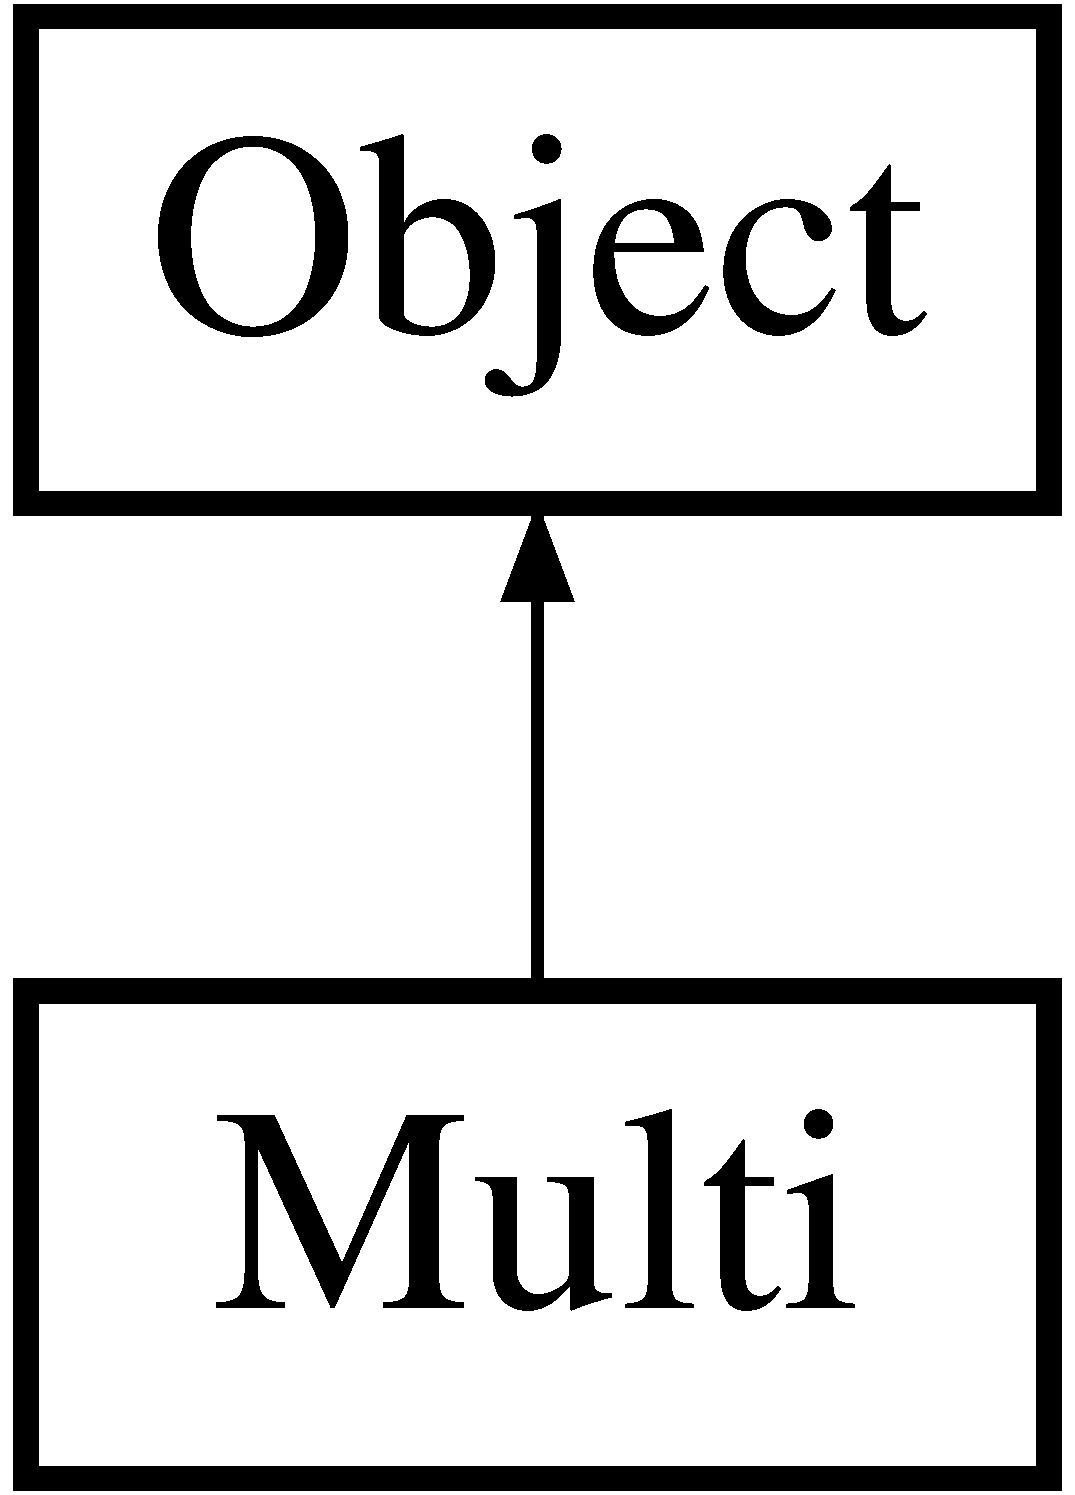
\includegraphics[height=2.000000cm]{class_multi}
\end{center}
\end{figure}
\subsection*{Public Member Functions}
\begin{DoxyCompactItemize}
\item 
\hyperlink{class_multi_a952193613f07eaeb1b75c7835955f169}{Multi} ()
\item 
\hyperlink{class_multi_a7d70368d5229d0ce1b0d735f15fbcd66}{Multi} (std\-::string file\-Name, std\-::map$<$ std\-::string, \hyperlink{class_object}{Object} $\ast$ $>$ $\ast$igraphs)
\item 
void \hyperlink{class_multi_a0b1957cf59a3d44294ddb35dadba199b}{draw} (float x, float y, float w, float h, std\-::string param)
\end{DoxyCompactItemize}


\subsection{Detailed Description}
Can draw parts of a \hyperlink{class_sprite}{Sprite} 

\subsection{Constructor \& Destructor Documentation}
\hypertarget{class_multi_a952193613f07eaeb1b75c7835955f169}{\index{Multi@{Multi}!Multi@{Multi}}
\index{Multi@{Multi}!Multi@{Multi}}
\subsubsection[{Multi}]{\setlength{\rightskip}{0pt plus 5cm}Multi\-::\-Multi (
\begin{DoxyParamCaption}
{}
\end{DoxyParamCaption}
)\hspace{0.3cm}{\ttfamily [inline]}}}\label{class_multi_a952193613f07eaeb1b75c7835955f169}
Default constructor \hypertarget{class_multi_a7d70368d5229d0ce1b0d735f15fbcd66}{\index{Multi@{Multi}!Multi@{Multi}}
\index{Multi@{Multi}!Multi@{Multi}}
\subsubsection[{Multi}]{\setlength{\rightskip}{0pt plus 5cm}Multi\-::\-Multi (
\begin{DoxyParamCaption}
\item[{std\-::string}]{file\-Name, }
\item[{std\-::map$<$ std\-::string, {\bf Object} $\ast$ $>$ $\ast$}]{igraphs}
\end{DoxyParamCaption}
)\hspace{0.3cm}{\ttfamily [inline]}}}\label{class_multi_a7d70368d5229d0ce1b0d735f15fbcd66}
Constructor 
\begin{DoxyParams}{Parameters}
{\em file\-Name} & name of multi file (.mlt) \\
\hline
{\em igraphs} & list of loaded graphics from \hyperlink{class_view}{View} class \\
\hline
\end{DoxyParams}


\subsection{Member Function Documentation}
\hypertarget{class_multi_a0b1957cf59a3d44294ddb35dadba199b}{\index{Multi@{Multi}!draw@{draw}}
\index{draw@{draw}!Multi@{Multi}}
\subsubsection[{draw}]{\setlength{\rightskip}{0pt plus 5cm}void Multi\-::draw (
\begin{DoxyParamCaption}
\item[{float}]{x, }
\item[{float}]{y, }
\item[{float}]{w, }
\item[{float}]{h, }
\item[{std\-::string}]{param}
\end{DoxyParamCaption}
)\hspace{0.3cm}{\ttfamily [virtual]}}}\label{class_multi_a0b1957cf59a3d44294ddb35dadba199b}
Draw a specific slice of a \hyperlink{class_sprite}{Sprite} 
\begin{DoxyParams}{Parameters}
{\em x} & coordinate \\
\hline
{\em y} & coordinate \\
\hline
{\em w} & width \\
\hline
{\em h} & height \\
\hline
{\em param} & full string param, determines which slice need to be drawn \\
\hline
\end{DoxyParams}


Reimplemented from \hyperlink{class_object_a13b99ec4da0a1c798104560c492c2a7e}{Object}.



The documentation for this class was generated from the following files\-:\begin{DoxyCompactItemize}
\item 
view/multi.\-h\item 
view/multi.\-cpp\end{DoxyCompactItemize}

\hypertarget{class_network}{\section{Network Class Reference}
\label{class_network}\index{Network@{Network}}
}


{\ttfamily \#include $<$network.\-h$>$}

\subsection*{Public Member Functions}
\begin{DoxyCompactItemize}
\item 
\hyperlink{class_network_a3cc2fb4f8fa4d507077e8da85ce5a1c8}{Network} ()
\item 
\hyperlink{class_network_a7a4e19cdb4bf0c7ecf82baa643831492}{$\sim$\-Network} ()
\item 
void \hyperlink{class_network_ad14847f8c3d10779a4fcaba08f88b6d6}{get\-Internet\-List} ()
\item 
void \hyperlink{class_network_a1b8853bc8d74bdc7e9fde02eacdf8cc2}{get\-Local\-List} ()
\item 
void \hyperlink{class_network_ab9fe53ec67f7eae4a1e01fd474590957}{start\-Listen} ()
\item 
void \hyperlink{class_network_ac45c78cca08f2123d9394a0a3c70d284}{stop\-Listen} ()
\item 
void \hyperlink{class_network_a6764800f1193201780329d32b1f0e10c}{connect} (std\-::string i\-Server\-Name)
\item 
void \hyperlink{class_network_ae44f73c87e85de6353c6365e5b86d911}{disconnect} ()
\item 
bool \hyperlink{class_network_a2f3a8809597f956dbf0c11a649ccf054}{send\-Packets} (std\-::vector$<$ \hyperlink{class_network_event}{Network\-Event} $>$ \&packets)
\item 
std\-::vector$<$ \hyperlink{class_network_event}{Network\-Event} $>$ \& \hyperlink{class_network_a6a85de91153350bca2776e092a524dd1}{get\-Packets} ()
\item 
void \hyperlink{class_network_a606848acb944241f270f52cd2a966b3b}{main\-Loop} ()
\item 
\hyperlink{class_server}{Server} \& \hyperlink{class_network_a6ec7cd6cb8fe04de45f6bf1e7efa8660}{get\-Server} ()
\item 
\hyperlink{class_client}{Client} \& \hyperlink{class_network_ab08b428a2f7cdbdf3cb7fd5e7e32d8ca}{get\-Client} ()
\item 
bool \hyperlink{class_network_a614afe83d863bafca483956b1ca43ca0}{get\-Success} () const 
\end{DoxyCompactItemize}


\subsection{Detailed Description}
Helper class to handle \hyperlink{class_server}{Server} and \hyperlink{class_client}{Client} together 

\subsection{Constructor \& Destructor Documentation}
\hypertarget{class_network_a3cc2fb4f8fa4d507077e8da85ce5a1c8}{\index{Network@{Network}!Network@{Network}}
\index{Network@{Network}!Network@{Network}}
\subsubsection[{Network}]{\setlength{\rightskip}{0pt plus 5cm}Network\-::\-Network (
\begin{DoxyParamCaption}
{}
\end{DoxyParamCaption}
)}}\label{class_network_a3cc2fb4f8fa4d507077e8da85ce5a1c8}
Constructor \hypertarget{class_network_a7a4e19cdb4bf0c7ecf82baa643831492}{\index{Network@{Network}!$\sim$\-Network@{$\sim$\-Network}}
\index{$\sim$\-Network@{$\sim$\-Network}!Network@{Network}}
\subsubsection[{$\sim$\-Network}]{\setlength{\rightskip}{0pt plus 5cm}Network\-::$\sim$\-Network (
\begin{DoxyParamCaption}
{}
\end{DoxyParamCaption}
)}}\label{class_network_a7a4e19cdb4bf0c7ecf82baa643831492}
Destructor 

\subsection{Member Function Documentation}
\hypertarget{class_network_a6764800f1193201780329d32b1f0e10c}{\index{Network@{Network}!connect@{connect}}
\index{connect@{connect}!Network@{Network}}
\subsubsection[{connect}]{\setlength{\rightskip}{0pt plus 5cm}void Network\-::connect (
\begin{DoxyParamCaption}
\item[{std\-::string}]{i\-Server\-Name}
\end{DoxyParamCaption}
)}}\label{class_network_a6764800f1193201780329d32b1f0e10c}
Connect to server \hypertarget{class_network_ae44f73c87e85de6353c6365e5b86d911}{\index{Network@{Network}!disconnect@{disconnect}}
\index{disconnect@{disconnect}!Network@{Network}}
\subsubsection[{disconnect}]{\setlength{\rightskip}{0pt plus 5cm}void Network\-::disconnect (
\begin{DoxyParamCaption}
{}
\end{DoxyParamCaption}
)}}\label{class_network_ae44f73c87e85de6353c6365e5b86d911}
Disconnect from server \hypertarget{class_network_ab08b428a2f7cdbdf3cb7fd5e7e32d8ca}{\index{Network@{Network}!get\-Client@{get\-Client}}
\index{get\-Client@{get\-Client}!Network@{Network}}
\subsubsection[{get\-Client}]{\setlength{\rightskip}{0pt plus 5cm}{\bf Client} \& Network\-::get\-Client (
\begin{DoxyParamCaption}
{}
\end{DoxyParamCaption}
)}}\label{class_network_ab08b428a2f7cdbdf3cb7fd5e7e32d8ca}
Get client class \hypertarget{class_network_ad14847f8c3d10779a4fcaba08f88b6d6}{\index{Network@{Network}!get\-Internet\-List@{get\-Internet\-List}}
\index{get\-Internet\-List@{get\-Internet\-List}!Network@{Network}}
\subsubsection[{get\-Internet\-List}]{\setlength{\rightskip}{0pt plus 5cm}void Network\-::get\-Internet\-List (
\begin{DoxyParamCaption}
{}
\end{DoxyParamCaption}
)}}\label{class_network_ad14847f8c3d10779a4fcaba08f88b6d6}
Get list of Internet servers \hypertarget{class_network_a1b8853bc8d74bdc7e9fde02eacdf8cc2}{\index{Network@{Network}!get\-Local\-List@{get\-Local\-List}}
\index{get\-Local\-List@{get\-Local\-List}!Network@{Network}}
\subsubsection[{get\-Local\-List}]{\setlength{\rightskip}{0pt plus 5cm}void Network\-::get\-Local\-List (
\begin{DoxyParamCaption}
{}
\end{DoxyParamCaption}
)}}\label{class_network_a1b8853bc8d74bdc7e9fde02eacdf8cc2}
Get lost of servers on local network \hypertarget{class_network_a6a85de91153350bca2776e092a524dd1}{\index{Network@{Network}!get\-Packets@{get\-Packets}}
\index{get\-Packets@{get\-Packets}!Network@{Network}}
\subsubsection[{get\-Packets}]{\setlength{\rightskip}{0pt plus 5cm}std\-::vector$<$ {\bf Network\-Event} $>$ \& Network\-::get\-Packets (
\begin{DoxyParamCaption}
{}
\end{DoxyParamCaption}
)}}\label{class_network_a6a85de91153350bca2776e092a524dd1}
Send packets where it is necessary \hypertarget{class_network_a6ec7cd6cb8fe04de45f6bf1e7efa8660}{\index{Network@{Network}!get\-Server@{get\-Server}}
\index{get\-Server@{get\-Server}!Network@{Network}}
\subsubsection[{get\-Server}]{\setlength{\rightskip}{0pt plus 5cm}{\bf Server} \& Network\-::get\-Server (
\begin{DoxyParamCaption}
{}
\end{DoxyParamCaption}
)}}\label{class_network_a6ec7cd6cb8fe04de45f6bf1e7efa8660}
Get server class \hypertarget{class_network_a614afe83d863bafca483956b1ca43ca0}{\index{Network@{Network}!get\-Success@{get\-Success}}
\index{get\-Success@{get\-Success}!Network@{Network}}
\subsubsection[{get\-Success}]{\setlength{\rightskip}{0pt plus 5cm}bool Network\-::get\-Success (
\begin{DoxyParamCaption}
{}
\end{DoxyParamCaption}
) const}}\label{class_network_a614afe83d863bafca483956b1ca43ca0}
False if error occured \hypertarget{class_network_a606848acb944241f270f52cd2a966b3b}{\index{Network@{Network}!main\-Loop@{main\-Loop}}
\index{main\-Loop@{main\-Loop}!Network@{Network}}
\subsubsection[{main\-Loop}]{\setlength{\rightskip}{0pt plus 5cm}void Network\-::main\-Loop (
\begin{DoxyParamCaption}
{}
\end{DoxyParamCaption}
)}}\label{class_network_a606848acb944241f270f52cd2a966b3b}
Main loop, for doing the work \hypertarget{class_network_a2f3a8809597f956dbf0c11a649ccf054}{\index{Network@{Network}!send\-Packets@{send\-Packets}}
\index{send\-Packets@{send\-Packets}!Network@{Network}}
\subsubsection[{send\-Packets}]{\setlength{\rightskip}{0pt plus 5cm}bool Network\-::send\-Packets (
\begin{DoxyParamCaption}
\item[{std\-::vector$<$ {\bf Network\-Event} $>$ \&}]{packets}
\end{DoxyParamCaption}
)}}\label{class_network_a2f3a8809597f956dbf0c11a649ccf054}
Send packets where it is necessary \hypertarget{class_network_ab9fe53ec67f7eae4a1e01fd474590957}{\index{Network@{Network}!start\-Listen@{start\-Listen}}
\index{start\-Listen@{start\-Listen}!Network@{Network}}
\subsubsection[{start\-Listen}]{\setlength{\rightskip}{0pt plus 5cm}void Network\-::start\-Listen (
\begin{DoxyParamCaption}
{}
\end{DoxyParamCaption}
)}}\label{class_network_ab9fe53ec67f7eae4a1e01fd474590957}
Start server \hypertarget{class_network_ac45c78cca08f2123d9394a0a3c70d284}{\index{Network@{Network}!stop\-Listen@{stop\-Listen}}
\index{stop\-Listen@{stop\-Listen}!Network@{Network}}
\subsubsection[{stop\-Listen}]{\setlength{\rightskip}{0pt plus 5cm}void Network\-::stop\-Listen (
\begin{DoxyParamCaption}
{}
\end{DoxyParamCaption}
)}}\label{class_network_ac45c78cca08f2123d9394a0a3c70d284}
Stop server 

The documentation for this class was generated from the following files\-:\begin{DoxyCompactItemize}
\item 
network.\-h\item 
network.\-cpp\end{DoxyCompactItemize}

\hypertarget{class_network_event}{\section{Network\-Event Class Reference}
\label{class_network_event}\index{Network\-Event@{Network\-Event}}
}


{\ttfamily \#include $<$networkevent.\-h$>$}

\subsection*{Public Member Functions}
\begin{DoxyCompactItemize}
\item 
\hyperlink{class_network_event_a6bcc9b872bba17dfd2923b66c42a2817}{Network\-Event} ()
\item 
\hyperlink{class_network_event_a81675f3074664bf4febfe56174d661ff}{Network\-Event} (E\-V\-E\-N\-T\-\_\-\-T\-Y\-P\-E e\-\_\-, unsigned char id\-\_\-, float x\-\_\-, float y\-\_\-)
\end{DoxyCompactItemize}
\subsection*{Public Attributes}
\begin{DoxyCompactItemize}
\item 
E\-V\-E\-N\-T\-\_\-\-T\-Y\-P\-E \hyperlink{class_network_event_a0f46f7a2c2876d3af113b5b50df06426}{e}
\item 
unsigned char \hyperlink{class_network_event_ac223ce8828eba29110147ed7a5a7d76b}{id}
\item 
float \hyperlink{class_network_event_ab847bb49581f345b762ba702fe41d505}{x}
\item 
float \hyperlink{class_network_event_ac12a2de372b8b3604b0f862a7e56e7dc}{y}
\end{DoxyCompactItemize}
\subsection*{Static Public Attributes}
\begin{DoxyCompactItemize}
\item 
static const int \hyperlink{class_network_event_a174f204e98eb4fd4fb442b9166208986}{packet\-Size} = 6
\end{DoxyCompactItemize}


\subsection{Detailed Description}
\hyperlink{class_network}{Network} packet, use \hyperlink{class_translate}{Translate} class to handle 

\subsection{Constructor \& Destructor Documentation}
\hypertarget{class_network_event_a6bcc9b872bba17dfd2923b66c42a2817}{\index{Network\-Event@{Network\-Event}!Network\-Event@{Network\-Event}}
\index{Network\-Event@{Network\-Event}!NetworkEvent@{Network\-Event}}
\subsubsection[{Network\-Event}]{\setlength{\rightskip}{0pt plus 5cm}Network\-Event\-::\-Network\-Event (
\begin{DoxyParamCaption}
{}
\end{DoxyParamCaption}
)\hspace{0.3cm}{\ttfamily [inline]}}}\label{class_network_event_a6bcc9b872bba17dfd2923b66c42a2817}
Default constructor \hypertarget{class_network_event_a81675f3074664bf4febfe56174d661ff}{\index{Network\-Event@{Network\-Event}!Network\-Event@{Network\-Event}}
\index{Network\-Event@{Network\-Event}!NetworkEvent@{Network\-Event}}
\subsubsection[{Network\-Event}]{\setlength{\rightskip}{0pt plus 5cm}Network\-Event\-::\-Network\-Event (
\begin{DoxyParamCaption}
\item[{E\-V\-E\-N\-T\-\_\-\-T\-Y\-P\-E}]{e\-\_\-, }
\item[{unsigned char}]{id\-\_\-, }
\item[{float}]{x\-\_\-, }
\item[{float}]{y\-\_\-}
\end{DoxyParamCaption}
)\hspace{0.3cm}{\ttfamily [inline]}}}\label{class_network_event_a81675f3074664bf4febfe56174d661ff}
Constructor 

\subsection{Member Data Documentation}
\hypertarget{class_network_event_a0f46f7a2c2876d3af113b5b50df06426}{\index{Network\-Event@{Network\-Event}!e@{e}}
\index{e@{e}!NetworkEvent@{Network\-Event}}
\subsubsection[{e}]{\setlength{\rightskip}{0pt plus 5cm}E\-V\-E\-N\-T\-\_\-\-T\-Y\-P\-E Network\-Event\-::e}}\label{class_network_event_a0f46f7a2c2876d3af113b5b50df06426}
Type of event \hypertarget{class_network_event_ac223ce8828eba29110147ed7a5a7d76b}{\index{Network\-Event@{Network\-Event}!id@{id}}
\index{id@{id}!NetworkEvent@{Network\-Event}}
\subsubsection[{id}]{\setlength{\rightskip}{0pt plus 5cm}unsigned char Network\-Event\-::id}}\label{class_network_event_ac223ce8828eba29110147ed7a5a7d76b}
I\-D of player (or monster) \hypertarget{class_network_event_a174f204e98eb4fd4fb442b9166208986}{\index{Network\-Event@{Network\-Event}!packet\-Size@{packet\-Size}}
\index{packet\-Size@{packet\-Size}!NetworkEvent@{Network\-Event}}
\subsubsection[{packet\-Size}]{\setlength{\rightskip}{0pt plus 5cm}const int Network\-Event\-::packet\-Size = 6\hspace{0.3cm}{\ttfamily [static]}}}\label{class_network_event_a174f204e98eb4fd4fb442b9166208986}
Size of all network packets \hypertarget{class_network_event_ab847bb49581f345b762ba702fe41d505}{\index{Network\-Event@{Network\-Event}!x@{x}}
\index{x@{x}!NetworkEvent@{Network\-Event}}
\subsubsection[{x}]{\setlength{\rightskip}{0pt plus 5cm}float Network\-Event\-::x}}\label{class_network_event_ab847bb49581f345b762ba702fe41d505}
Coordinate X \hypertarget{class_network_event_ac12a2de372b8b3604b0f862a7e56e7dc}{\index{Network\-Event@{Network\-Event}!y@{y}}
\index{y@{y}!NetworkEvent@{Network\-Event}}
\subsubsection[{y}]{\setlength{\rightskip}{0pt plus 5cm}float Network\-Event\-::y}}\label{class_network_event_ac12a2de372b8b3604b0f862a7e56e7dc}
Coordinate Y 

The documentation for this class was generated from the following file\-:\begin{DoxyCompactItemize}
\item 
networkevent.\-h\end{DoxyCompactItemize}

\hypertarget{class_object}{\section{Object Class Reference}
\label{class_object}\index{Object@{Object}}
}


{\ttfamily \#include $<$object.\-h$>$}

Inheritance diagram for Object\-:\begin{figure}[H]
\begin{center}
\leavevmode
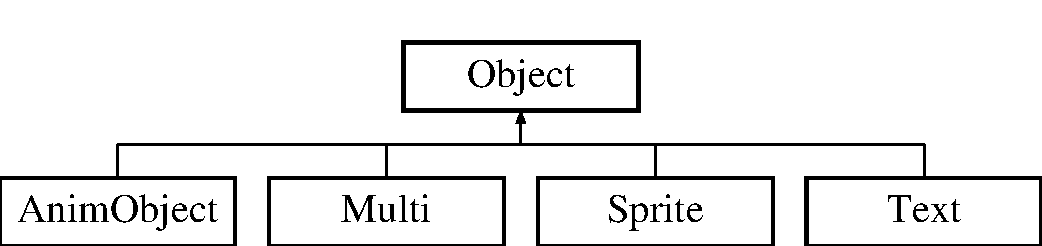
\includegraphics[height=2.000000cm]{class_object}
\end{center}
\end{figure}
\subsection*{Public Member Functions}
\begin{DoxyCompactItemize}
\item 
virtual void \hyperlink{class_object_a13b99ec4da0a1c798104560c492c2a7e}{draw} (float x, float y, float w, float h, std\-::string param=\char`\"{}\char`\"{})
\item 
virtual void \hyperlink{class_object_a210c8bac4e5705ffee71d0837e46ab46}{bind} ()
\item 
virtual \hyperlink{class_object_aa3e791419d84c4c346ef9499513b8e00}{$\sim$\-Object} ()
\end{DoxyCompactItemize}


\subsection{Detailed Description}
Base class of drawable objects 

\subsection{Constructor \& Destructor Documentation}
\hypertarget{class_object_aa3e791419d84c4c346ef9499513b8e00}{\index{Object@{Object}!$\sim$\-Object@{$\sim$\-Object}}
\index{$\sim$\-Object@{$\sim$\-Object}!Object@{Object}}
\subsubsection[{$\sim$\-Object}]{\setlength{\rightskip}{0pt plus 5cm}virtual Object\-::$\sim$\-Object (
\begin{DoxyParamCaption}
{}
\end{DoxyParamCaption}
)\hspace{0.3cm}{\ttfamily [inline]}, {\ttfamily [virtual]}}}\label{class_object_aa3e791419d84c4c346ef9499513b8e00}
Destructor 

\subsection{Member Function Documentation}
\hypertarget{class_object_a210c8bac4e5705ffee71d0837e46ab46}{\index{Object@{Object}!bind@{bind}}
\index{bind@{bind}!Object@{Object}}
\subsubsection[{bind}]{\setlength{\rightskip}{0pt plus 5cm}virtual void Object\-::bind (
\begin{DoxyParamCaption}
{}
\end{DoxyParamCaption}
)\hspace{0.3cm}{\ttfamily [inline]}, {\ttfamily [virtual]}}}\label{class_object_a210c8bac4e5705ffee71d0837e46ab46}
Bind graphic to draw texture 

Reimplemented in \hyperlink{class_sprite_a3689496f6c44c2c6fd9dd6bd92bf1742}{Sprite}.

\hypertarget{class_object_a13b99ec4da0a1c798104560c492c2a7e}{\index{Object@{Object}!draw@{draw}}
\index{draw@{draw}!Object@{Object}}
\subsubsection[{draw}]{\setlength{\rightskip}{0pt plus 5cm}virtual void Object\-::draw (
\begin{DoxyParamCaption}
\item[{float}]{x, }
\item[{float}]{y, }
\item[{float}]{w, }
\item[{float}]{h, }
\item[{std\-::string}]{param = {\ttfamily \char`\"{}\char`\"{}}}
\end{DoxyParamCaption}
)\hspace{0.3cm}{\ttfamily [inline]}, {\ttfamily [virtual]}}}\label{class_object_a13b99ec4da0a1c798104560c492c2a7e}
Drawing object on screen 
\begin{DoxyParams}{Parameters}
{\em x} & coordinate \\
\hline
{\em y} & coordinate \\
\hline
{\em w} & width \\
\hline
{\em h} & height \\
\hline
{\em param} & full drawing string \\
\hline
\end{DoxyParams}


Reimplemented in \hyperlink{class_sprite_a0d00170fb8cc22361e2c16c4b3818e7e}{Sprite}, \hyperlink{class_text_a7eb6b5f04d40c5f3f482413612d0a101}{Text}, \hyperlink{class_anim_object_a93eda4562497de04bf7db6407d74e5aa}{Anim\-Object}, and \hyperlink{class_multi_a0b1957cf59a3d44294ddb35dadba199b}{Multi}.



The documentation for this class was generated from the following file\-:\begin{DoxyCompactItemize}
\item 
view/object.\-h\end{DoxyCompactItemize}

\hypertarget{class_player}{\section{Player Class Reference}
\label{class_player}\index{Player@{Player}}
}


{\ttfamily \#include $<$player.\-h$>$}

\subsection*{Public Member Functions}
\begin{DoxyCompactItemize}
\item 
\hyperlink{class_player_affe0cc3cb714f6deb4e62f0c0d3f1fd8}{Player} ()
\item 
\hyperlink{class_player_a749d2c00e1fe0f5c2746f7505a58c062}{$\sim$\-Player} ()
\item 
void \hyperlink{class_player_a015ea21fa1e7273e47d48cb20d9b12e3}{init} ()
\item 
void \hyperlink{class_player_ac9fcb79ecfc70a168f1bb906f2fe0877}{new\-Round} ()
\item 
void \hyperlink{class_player_ae9b137fafb1897951e079b5fd373d2f9}{novirus} ()
\item 
void \hyperlink{class_player_aa7f367a180d810ca39375a22fbaba45e}{move} (T\-I\-M\-E inow)
\item 
void \hyperlink{class_player_ab0f0baae5dabefc1022f7d5eec563aaa}{move} (\hyperlink{class_point}{Point}$<$ float $>$ p, T\-I\-M\-E inow)
\item 
bool \hyperlink{class_player_a993141b4f86b25982389ae524bffc915}{get\-Move} (\hyperlink{class_point}{Point}$<$ float $>$ \&p)
\item 
int \hyperlink{class_player_a865d5ca25d1d90a9b046507a0bd63dec}{infect} (int type)
\item 
void \hyperlink{class_player_a1e4b3e6ef91fc400ff2c6c26b1370f8c}{die} ()
\item 
void \hyperlink{class_player_a5d5f04fda1a8534138cd75077192c648}{win} ()
\item 
std\-::string \hyperlink{class_player_a316c65f3722a618f53139beb1248ea8f}{state} ()
\item 
std\-::string \hyperlink{class_player_a0194487be45d72dd9601a02f70a2454b}{get\-Aura} () const 
\item 
bool \hyperlink{class_player_a811626a8360d14d19f6e5e59c4b7f2ad}{get\-Put} () const 
\item 
bool \hyperlink{class_player_aeeda5dfdf5c3c53f3e09515fbf8e04cb}{get\-Put\-Force} () const 
\item 
int \hyperlink{class_player_afc6b4cc3a34e9b01f9f8659f5d9f62ec}{get\-Id} () const 
\item 
\hyperlink{class_control}{Control} $\ast$ \hyperlink{class_player_a177fc4573489be6bfced432d42dc9901}{get\-Control} ()
\item 
\hyperlink{class_point}{Point}$<$ float $>$ \hyperlink{class_player_ab0cd970c56e92afbb670ff92420cc620}{get\-Point} ()
\item 
float \hyperlink{class_player_a0a7dadbb84ba8e0d6688905cd1f33907}{get\-X} ()
\item 
float \hyperlink{class_player_a320d19fb4d116cb0bbe93ebd83401ee8}{get\-Y} ()
\item 
float \hyperlink{class_player_a19718078a93e54d5d642ada0a0e4720f}{get\-Prev\-X} ()
\item 
float \hyperlink{class_player_a033a3bfcecfba4fa915843e30b2f5ad8}{get\-Prev\-Y} ()
\item 
int \hyperlink{class_player_a3b1247033f5b70a95a18f8b3dc340ac4}{get\-Bomb\-X} ()
\item 
int \hyperlink{class_player_adf6b9c031c4f910356154868e5a1ce94}{get\-Bomb\-Y} ()
\item 
int \hyperlink{class_player_a5ac337bd1d470a1e2056ef5f733b4a05}{get\-Size} ()
\item 
int \hyperlink{class_player_ad033c753ad4551e741386f47efe8c5f5}{get\-Bombs} ()
\item 
int \hyperlink{class_player_a6869c0d8d0f77d6a25a5f511a3b127c7}{get\-Life} () const 
\item 
bool \hyperlink{class_player_a6bbe79e1857b945a3472beadccb32025}{is\-Alive} () const 
\item 
int \hyperlink{class_player_ac10eb9fb0387f565134958d129585ac6}{get\-Score} () const 
\item 
int \hyperlink{class_player_a37ce1500bd1bde0e6a38521b8a6ae5e3}{get\-Kill} () const 
\item 
int \hyperlink{class_player_a2249acef49eddb2aa28e52fb2b48d543}{get\-Killed} () const 
\item 
int \hyperlink{class_player_afd3d5494e20b82628ad16b6b9e076de5}{get\-Monster\-Kill} () const 
\item 
bool \hyperlink{class_player_a7db9e6e10fec7d36b2dab1268f405f68}{get\-Remote} () const 
\item 
std\-::string \hyperlink{class_player_aaa92b93cc17660bf094225dccc749583}{get\-Skin} () const 
\item 
int \hyperlink{class_player_ac8a09e2197142d048b0992ad770c08cd}{get\-Team} () const 
\item 
T\-I\-M\-E \hyperlink{class_player_a21745d8c82684a875a22609070c814cb}{get\-Die} () const 
\item 
T\-I\-M\-E \hyperlink{class_player_a591f6c56e5779c24f5477fc8b5d926e9}{get\-Show\-Kills} () const 
\item 
void \hyperlink{class_player_aa2cb5c8fe89f6f37f99abe6df7199fc1}{set\-Id} (int i)
\item 
void \hyperlink{class_player_a03591edbf27ba278d59af89e7fce4c32}{set\-Control} (\hyperlink{class_control}{Control} $\ast$icontrol)
\item 
void \hyperlink{class_player_a8b75c659b6f39a5abb564f29fc856ed4}{set\-X} (float x)
\item 
void \hyperlink{class_player_aeb1f6a2fee6b2ce819fed37fe9f21890}{set\-Y} (float y)
\item 
void \hyperlink{class_player_af3e70ea08d33b6c551d8777fafd677ae}{set\-Bomb\-X} (int x)
\item 
void \hyperlink{class_player_ad1742f6e29e3589746a59bad9de7e5f3}{set\-Bomb\-Y} (int y)
\item 
void \hyperlink{class_player_a0be84429f8bd31b22fae60f943affc1d}{inc\-Size} ()
\item 
void \hyperlink{class_player_abce1145d360ac0d240a78d5d4ea92dd3}{inc\-Bombs} ()
\item 
void \hyperlink{class_player_a132902f4b3306708346e22b4338428d4}{dec\-Bombs} ()
\item 
void \hyperlink{class_player_a4cdcb55d3d63a2ee67a01526a8a00a24}{set\-Life} (int l)
\item 
void \hyperlink{class_player_a0932a3bfeecbad1f64a9ecf364de1da8}{set\-Put} (bool p)
\item 
void \hyperlink{class_player_a85509b879f09e56aef34a09f0ac8d6df}{set\-Score} (int s)
\item 
void \hyperlink{class_player_a86da21ed2e4b6e6dcd0609f4666e3f98}{inc\-Score} ()
\item 
void \hyperlink{class_player_adc5ca4d3051a2240b40e9e8eeaf3919d}{set\-Kill} (int k)
\item 
void \hyperlink{class_player_ab0ff3a991f415db0c754bd15ef7f7632}{inc\-Kill} ()
\item 
void \hyperlink{class_player_a2a63a9b8decaf0254d657bf575f55c73}{inc\-Kill} (T\-I\-M\-E i\-Show\-Kills)
\item 
void \hyperlink{class_player_a41d67486b2e82e32286ca93f58f266be}{dec\-Kill} ()
\item 
void \hyperlink{class_player_a3be7e0463c2ac7c8ebd5bdf218ffa945}{dec\-Kill} (T\-I\-M\-E i\-Show\-Kills)
\item 
void \hyperlink{class_player_a557158a867fd435099818246c467771e}{set\-Show\-Kills} (T\-I\-M\-E i\-Show\-Kills)
\item 
void \hyperlink{class_player_ab661c93ec708508b3d63207de3ceb007}{set\-Show\-Kills} (T\-I\-M\-E i\-Show\-Kills, int number)
\item 
void \hyperlink{class_player_a80c1d3984b93a61e7d6e4e8d1db1cc0e}{set\-Killed} (int k)
\item 
void \hyperlink{class_player_a2e22e37e13a43cb7253802b8ac99a159}{inc\-Killed} ()
\item 
void \hyperlink{class_player_ac99bd37b81f07de6ad6268217dc28b42}{set\-Monster\-Kill} (int k)
\item 
void \hyperlink{class_player_aa6fb55ce0e5f324a0d21a67b4f64e287}{inc\-Monster\-Kill} ()
\item 
void \hyperlink{class_player_a0056f65dd63470c8a676c3d0417fbe9f}{set\-Remote} (bool i\-Remote)
\item 
void \hyperlink{class_player_a6022b2097c1330fc70f19745210ddf39}{set\-Skin} (std\-::string i\-Skin)
\item 
void \hyperlink{class_player_a4cfd169b16a49c4323de4ed14f4ea910}{set\-Team} (int iteam)
\item 
void \hyperlink{class_player_afd8af484ccdcec04bd881df1e572be39}{set\-Die} (T\-I\-M\-E idie)
\item 
void \hyperlink{class_player_a2dd87cb4c6d9fec37b12ed005b143260}{set\-Start} (\hyperlink{class_point}{Point}$<$ float $>$ p, T\-I\-M\-E t)
\item 
void \hyperlink{class_player_a99088f2db619e4534f610a68c381bd54}{set\-Start} (T\-I\-M\-E t)
\item 
bool \hyperlink{class_player_a948d84f95ca15f0cba6f868f17429174}{is\-Immortal} () const 
\item 
bool \hyperlink{class_player_a58f1e0d5e4a5788824e416c492f41563}{is\-Remote\-Player} () const 
\item 
bool \hyperlink{class_player_a6b9b7eb45cf04d35dc0e930882a1e229}{get\-Send\-Show\-Kills} ()
\item 
int \hyperlink{class_player_a201ff389388118fb8e2dcb2aac14424e}{get\-Received\-Show\-Kills} () const 
\end{DoxyCompactItemize}


\subsection{Detailed Description}
This class contains all information about a player 

\subsection{Constructor \& Destructor Documentation}
\hypertarget{class_player_affe0cc3cb714f6deb4e62f0c0d3f1fd8}{\index{Player@{Player}!Player@{Player}}
\index{Player@{Player}!Player@{Player}}
\subsubsection[{Player}]{\setlength{\rightskip}{0pt plus 5cm}Player\-::\-Player (
\begin{DoxyParamCaption}
{}
\end{DoxyParamCaption}
)}}\label{class_player_affe0cc3cb714f6deb4e62f0c0d3f1fd8}
Constructor, initialize player \hypertarget{class_player_a749d2c00e1fe0f5c2746f7505a58c062}{\index{Player@{Player}!$\sim$\-Player@{$\sim$\-Player}}
\index{$\sim$\-Player@{$\sim$\-Player}!Player@{Player}}
\subsubsection[{$\sim$\-Player}]{\setlength{\rightskip}{0pt plus 5cm}Player\-::$\sim$\-Player (
\begin{DoxyParamCaption}
{}
\end{DoxyParamCaption}
)}}\label{class_player_a749d2c00e1fe0f5c2746f7505a58c062}
Destructor 

\subsection{Member Function Documentation}
\hypertarget{class_player_a132902f4b3306708346e22b4338428d4}{\index{Player@{Player}!dec\-Bombs@{dec\-Bombs}}
\index{dec\-Bombs@{dec\-Bombs}!Player@{Player}}
\subsubsection[{dec\-Bombs}]{\setlength{\rightskip}{0pt plus 5cm}void Player\-::dec\-Bombs (
\begin{DoxyParamCaption}
{}
\end{DoxyParamCaption}
)\hspace{0.3cm}{\ttfamily [inline]}}}\label{class_player_a132902f4b3306708346e22b4338428d4}
Decrease number of bombs \hypertarget{class_player_a41d67486b2e82e32286ca93f58f266be}{\index{Player@{Player}!dec\-Kill@{dec\-Kill}}
\index{dec\-Kill@{dec\-Kill}!Player@{Player}}
\subsubsection[{dec\-Kill}]{\setlength{\rightskip}{0pt plus 5cm}void Player\-::dec\-Kill (
\begin{DoxyParamCaption}
{}
\end{DoxyParamCaption}
)\hspace{0.3cm}{\ttfamily [inline]}}}\label{class_player_a41d67486b2e82e32286ca93f58f266be}
Decrease kills (when suicide) \hypertarget{class_player_a3be7e0463c2ac7c8ebd5bdf218ffa945}{\index{Player@{Player}!dec\-Kill@{dec\-Kill}}
\index{dec\-Kill@{dec\-Kill}!Player@{Player}}
\subsubsection[{dec\-Kill}]{\setlength{\rightskip}{0pt plus 5cm}void Player\-::dec\-Kill (
\begin{DoxyParamCaption}
\item[{T\-I\-M\-E}]{i\-Show\-Kills}
\end{DoxyParamCaption}
)\hspace{0.3cm}{\ttfamily [inline]}}}\label{class_player_a3be7e0463c2ac7c8ebd5bdf218ffa945}
Decrease kills (when suicide) with showing the statistics 
\begin{DoxyParams}{Parameters}
{\em i\-Show\-Kills} & frame time when it should disappear \\
\hline
\end{DoxyParams}
\hypertarget{class_player_a1e4b3e6ef91fc400ff2c6c26b1370f8c}{\index{Player@{Player}!die@{die}}
\index{die@{die}!Player@{Player}}
\subsubsection[{die}]{\setlength{\rightskip}{0pt plus 5cm}void Player\-::die (
\begin{DoxyParamCaption}
{}
\end{DoxyParamCaption}
)}}\label{class_player_a1e4b3e6ef91fc400ff2c6c26b1370f8c}
\hyperlink{class_player}{Player} dies \hypertarget{class_player_a0194487be45d72dd9601a02f70a2454b}{\index{Player@{Player}!get\-Aura@{get\-Aura}}
\index{get\-Aura@{get\-Aura}!Player@{Player}}
\subsubsection[{get\-Aura}]{\setlength{\rightskip}{0pt plus 5cm}std\-::string Player\-::get\-Aura (
\begin{DoxyParamCaption}
{}
\end{DoxyParamCaption}
) const}}\label{class_player_a0194487be45d72dd9601a02f70a2454b}
Get special effect around player \begin{DoxyReturn}{Returns}
graphic name 
\end{DoxyReturn}
\hypertarget{class_player_ad033c753ad4551e741386f47efe8c5f5}{\index{Player@{Player}!get\-Bombs@{get\-Bombs}}
\index{get\-Bombs@{get\-Bombs}!Player@{Player}}
\subsubsection[{get\-Bombs}]{\setlength{\rightskip}{0pt plus 5cm}int Player\-::get\-Bombs (
\begin{DoxyParamCaption}
{}
\end{DoxyParamCaption}
)\hspace{0.3cm}{\ttfamily [inline]}}}\label{class_player_ad033c753ad4551e741386f47efe8c5f5}
Get number of bombs \hypertarget{class_player_a3b1247033f5b70a95a18f8b3dc340ac4}{\index{Player@{Player}!get\-Bomb\-X@{get\-Bomb\-X}}
\index{get\-Bomb\-X@{get\-Bomb\-X}!Player@{Player}}
\subsubsection[{get\-Bomb\-X}]{\setlength{\rightskip}{0pt plus 5cm}int Player\-::get\-Bomb\-X (
\begin{DoxyParamCaption}
{}
\end{DoxyParamCaption}
)\hspace{0.3cm}{\ttfamily [inline]}}}\label{class_player_a3b1247033f5b70a95a18f8b3dc340ac4}
Get the X coordinate where the player put bomb \hypertarget{class_player_adf6b9c031c4f910356154868e5a1ce94}{\index{Player@{Player}!get\-Bomb\-Y@{get\-Bomb\-Y}}
\index{get\-Bomb\-Y@{get\-Bomb\-Y}!Player@{Player}}
\subsubsection[{get\-Bomb\-Y}]{\setlength{\rightskip}{0pt plus 5cm}int Player\-::get\-Bomb\-Y (
\begin{DoxyParamCaption}
{}
\end{DoxyParamCaption}
)\hspace{0.3cm}{\ttfamily [inline]}}}\label{class_player_adf6b9c031c4f910356154868e5a1ce94}
Get the Y coordinate where the player put bomb \hypertarget{class_player_a177fc4573489be6bfced432d42dc9901}{\index{Player@{Player}!get\-Control@{get\-Control}}
\index{get\-Control@{get\-Control}!Player@{Player}}
\subsubsection[{get\-Control}]{\setlength{\rightskip}{0pt plus 5cm}{\bf Control}$\ast$ Player\-::get\-Control (
\begin{DoxyParamCaption}
{}
\end{DoxyParamCaption}
)\hspace{0.3cm}{\ttfamily [inline]}}}\label{class_player_a177fc4573489be6bfced432d42dc9901}
Returns the \hyperlink{class_control}{Control} class of player \hypertarget{class_player_a21745d8c82684a875a22609070c814cb}{\index{Player@{Player}!get\-Die@{get\-Die}}
\index{get\-Die@{get\-Die}!Player@{Player}}
\subsubsection[{get\-Die}]{\setlength{\rightskip}{0pt plus 5cm}T\-I\-M\-E Player\-::get\-Die (
\begin{DoxyParamCaption}
{}
\end{DoxyParamCaption}
) const\hspace{0.3cm}{\ttfamily [inline]}}}\label{class_player_a21745d8c82684a875a22609070c814cb}
Return the frame time when player died \hypertarget{class_player_afc6b4cc3a34e9b01f9f8659f5d9f62ec}{\index{Player@{Player}!get\-Id@{get\-Id}}
\index{get\-Id@{get\-Id}!Player@{Player}}
\subsubsection[{get\-Id}]{\setlength{\rightskip}{0pt plus 5cm}int Player\-::get\-Id (
\begin{DoxyParamCaption}
{}
\end{DoxyParamCaption}
) const\hspace{0.3cm}{\ttfamily [inline]}}}\label{class_player_afc6b4cc3a34e9b01f9f8659f5d9f62ec}
Return the I\-D of the player \hypertarget{class_player_a37ce1500bd1bde0e6a38521b8a6ae5e3}{\index{Player@{Player}!get\-Kill@{get\-Kill}}
\index{get\-Kill@{get\-Kill}!Player@{Player}}
\subsubsection[{get\-Kill}]{\setlength{\rightskip}{0pt plus 5cm}int Player\-::get\-Kill (
\begin{DoxyParamCaption}
{}
\end{DoxyParamCaption}
) const\hspace{0.3cm}{\ttfamily [inline]}}}\label{class_player_a37ce1500bd1bde0e6a38521b8a6ae5e3}
Get the number of kills \hypertarget{class_player_a2249acef49eddb2aa28e52fb2b48d543}{\index{Player@{Player}!get\-Killed@{get\-Killed}}
\index{get\-Killed@{get\-Killed}!Player@{Player}}
\subsubsection[{get\-Killed}]{\setlength{\rightskip}{0pt plus 5cm}int Player\-::get\-Killed (
\begin{DoxyParamCaption}
{}
\end{DoxyParamCaption}
) const\hspace{0.3cm}{\ttfamily [inline]}}}\label{class_player_a2249acef49eddb2aa28e52fb2b48d543}
Get the number of get killed \hypertarget{class_player_a6869c0d8d0f77d6a25a5f511a3b127c7}{\index{Player@{Player}!get\-Life@{get\-Life}}
\index{get\-Life@{get\-Life}!Player@{Player}}
\subsubsection[{get\-Life}]{\setlength{\rightskip}{0pt plus 5cm}int Player\-::get\-Life (
\begin{DoxyParamCaption}
{}
\end{DoxyParamCaption}
) const\hspace{0.3cm}{\ttfamily [inline]}}}\label{class_player_a6869c0d8d0f77d6a25a5f511a3b127c7}
Get life of player \hypertarget{class_player_afd3d5494e20b82628ad16b6b9e076de5}{\index{Player@{Player}!get\-Monster\-Kill@{get\-Monster\-Kill}}
\index{get\-Monster\-Kill@{get\-Monster\-Kill}!Player@{Player}}
\subsubsection[{get\-Monster\-Kill}]{\setlength{\rightskip}{0pt plus 5cm}int Player\-::get\-Monster\-Kill (
\begin{DoxyParamCaption}
{}
\end{DoxyParamCaption}
) const\hspace{0.3cm}{\ttfamily [inline]}}}\label{class_player_afd3d5494e20b82628ad16b6b9e076de5}
Get the number of monsters killed \hypertarget{class_player_a993141b4f86b25982389ae524bffc915}{\index{Player@{Player}!get\-Move@{get\-Move}}
\index{get\-Move@{get\-Move}!Player@{Player}}
\subsubsection[{get\-Move}]{\setlength{\rightskip}{0pt plus 5cm}bool Player\-::get\-Move (
\begin{DoxyParamCaption}
\item[{{\bf Point}$<$ float $>$ \&}]{p}
\end{DoxyParamCaption}
)}}\label{class_player_a993141b4f86b25982389ae524bffc915}
Get movement of player. 
\begin{DoxyParams}{Parameters}
{\em p} & the new position \\
\hline
\end{DoxyParams}
\begin{DoxyReturn}{Returns}
the player changes it's position or not 
\end{DoxyReturn}
\hypertarget{class_player_ab0cd970c56e92afbb670ff92420cc620}{\index{Player@{Player}!get\-Point@{get\-Point}}
\index{get\-Point@{get\-Point}!Player@{Player}}
\subsubsection[{get\-Point}]{\setlength{\rightskip}{0pt plus 5cm}{\bf Point}$<$float$>$ Player\-::get\-Point (
\begin{DoxyParamCaption}
{}
\end{DoxyParamCaption}
)\hspace{0.3cm}{\ttfamily [inline]}}}\label{class_player_ab0cd970c56e92afbb670ff92420cc620}
Get position of player \hypertarget{class_player_a19718078a93e54d5d642ada0a0e4720f}{\index{Player@{Player}!get\-Prev\-X@{get\-Prev\-X}}
\index{get\-Prev\-X@{get\-Prev\-X}!Player@{Player}}
\subsubsection[{get\-Prev\-X}]{\setlength{\rightskip}{0pt plus 5cm}float Player\-::get\-Prev\-X (
\begin{DoxyParamCaption}
{}
\end{DoxyParamCaption}
)\hspace{0.3cm}{\ttfamily [inline]}}}\label{class_player_a19718078a93e54d5d642ada0a0e4720f}
Get previous X coordinate of player \hypertarget{class_player_a033a3bfcecfba4fa915843e30b2f5ad8}{\index{Player@{Player}!get\-Prev\-Y@{get\-Prev\-Y}}
\index{get\-Prev\-Y@{get\-Prev\-Y}!Player@{Player}}
\subsubsection[{get\-Prev\-Y}]{\setlength{\rightskip}{0pt plus 5cm}float Player\-::get\-Prev\-Y (
\begin{DoxyParamCaption}
{}
\end{DoxyParamCaption}
)\hspace{0.3cm}{\ttfamily [inline]}}}\label{class_player_a033a3bfcecfba4fa915843e30b2f5ad8}
Get previous Y coordinate of player \hypertarget{class_player_a811626a8360d14d19f6e5e59c4b7f2ad}{\index{Player@{Player}!get\-Put@{get\-Put}}
\index{get\-Put@{get\-Put}!Player@{Player}}
\subsubsection[{get\-Put}]{\setlength{\rightskip}{0pt plus 5cm}bool Player\-::get\-Put (
\begin{DoxyParamCaption}
{}
\end{DoxyParamCaption}
) const}}\label{class_player_a811626a8360d14d19f6e5e59c4b7f2ad}
Return that the player puts bomb or not \hypertarget{class_player_aeeda5dfdf5c3c53f3e09515fbf8e04cb}{\index{Player@{Player}!get\-Put\-Force@{get\-Put\-Force}}
\index{get\-Put\-Force@{get\-Put\-Force}!Player@{Player}}
\subsubsection[{get\-Put\-Force}]{\setlength{\rightskip}{0pt plus 5cm}bool Player\-::get\-Put\-Force (
\begin{DoxyParamCaption}
{}
\end{DoxyParamCaption}
) const}}\label{class_player_aeeda5dfdf5c3c53f3e09515fbf8e04cb}
Return in any case that the player puts bomb or not (for scoreboard skip) \hypertarget{class_player_a201ff389388118fb8e2dcb2aac14424e}{\index{Player@{Player}!get\-Received\-Show\-Kills@{get\-Received\-Show\-Kills}}
\index{get\-Received\-Show\-Kills@{get\-Received\-Show\-Kills}!Player@{Player}}
\subsubsection[{get\-Received\-Show\-Kills}]{\setlength{\rightskip}{0pt plus 5cm}int Player\-::get\-Received\-Show\-Kills (
\begin{DoxyParamCaption}
{}
\end{DoxyParamCaption}
) const\hspace{0.3cm}{\ttfamily [inline]}}}\label{class_player_a201ff389388118fb8e2dcb2aac14424e}
For client, return the data to show on table \hypertarget{class_player_a7db9e6e10fec7d36b2dab1268f405f68}{\index{Player@{Player}!get\-Remote@{get\-Remote}}
\index{get\-Remote@{get\-Remote}!Player@{Player}}
\subsubsection[{get\-Remote}]{\setlength{\rightskip}{0pt plus 5cm}bool Player\-::get\-Remote (
\begin{DoxyParamCaption}
{}
\end{DoxyParamCaption}
) const\hspace{0.3cm}{\ttfamily [inline]}}}\label{class_player_a7db9e6e10fec7d36b2dab1268f405f68}
Get if the player is remote \hypertarget{class_player_ac10eb9fb0387f565134958d129585ac6}{\index{Player@{Player}!get\-Score@{get\-Score}}
\index{get\-Score@{get\-Score}!Player@{Player}}
\subsubsection[{get\-Score}]{\setlength{\rightskip}{0pt plus 5cm}int Player\-::get\-Score (
\begin{DoxyParamCaption}
{}
\end{DoxyParamCaption}
) const\hspace{0.3cm}{\ttfamily [inline]}}}\label{class_player_ac10eb9fb0387f565134958d129585ac6}
Get score of player \hypertarget{class_player_a6b9b7eb45cf04d35dc0e930882a1e229}{\index{Player@{Player}!get\-Send\-Show\-Kills@{get\-Send\-Show\-Kills}}
\index{get\-Send\-Show\-Kills@{get\-Send\-Show\-Kills}!Player@{Player}}
\subsubsection[{get\-Send\-Show\-Kills}]{\setlength{\rightskip}{0pt plus 5cm}bool Player\-::get\-Send\-Show\-Kills (
\begin{DoxyParamCaption}
{}
\end{DoxyParamCaption}
)\hspace{0.3cm}{\ttfamily [inline]}}}\label{class_player_a6b9b7eb45cf04d35dc0e930882a1e229}
True if show kills changed and needs to be sent \hypertarget{class_player_a591f6c56e5779c24f5477fc8b5d926e9}{\index{Player@{Player}!get\-Show\-Kills@{get\-Show\-Kills}}
\index{get\-Show\-Kills@{get\-Show\-Kills}!Player@{Player}}
\subsubsection[{get\-Show\-Kills}]{\setlength{\rightskip}{0pt plus 5cm}T\-I\-M\-E Player\-::get\-Show\-Kills (
\begin{DoxyParamCaption}
{}
\end{DoxyParamCaption}
) const\hspace{0.3cm}{\ttfamily [inline]}}}\label{class_player_a591f6c56e5779c24f5477fc8b5d926e9}
Return when showing kill statistic should disappear \hypertarget{class_player_a5ac337bd1d470a1e2056ef5f733b4a05}{\index{Player@{Player}!get\-Size@{get\-Size}}
\index{get\-Size@{get\-Size}!Player@{Player}}
\subsubsection[{get\-Size}]{\setlength{\rightskip}{0pt plus 5cm}int Player\-::get\-Size (
\begin{DoxyParamCaption}
{}
\end{DoxyParamCaption}
)\hspace{0.3cm}{\ttfamily [inline]}}}\label{class_player_a5ac337bd1d470a1e2056ef5f733b4a05}
Get flame size \hypertarget{class_player_aaa92b93cc17660bf094225dccc749583}{\index{Player@{Player}!get\-Skin@{get\-Skin}}
\index{get\-Skin@{get\-Skin}!Player@{Player}}
\subsubsection[{get\-Skin}]{\setlength{\rightskip}{0pt plus 5cm}std\-::string Player\-::get\-Skin (
\begin{DoxyParamCaption}
{}
\end{DoxyParamCaption}
) const\hspace{0.3cm}{\ttfamily [inline]}}}\label{class_player_aaa92b93cc17660bf094225dccc749583}
Get skin of player (prefix for graphic files) \hypertarget{class_player_ac8a09e2197142d048b0992ad770c08cd}{\index{Player@{Player}!get\-Team@{get\-Team}}
\index{get\-Team@{get\-Team}!Player@{Player}}
\subsubsection[{get\-Team}]{\setlength{\rightskip}{0pt plus 5cm}int Player\-::get\-Team (
\begin{DoxyParamCaption}
{}
\end{DoxyParamCaption}
) const\hspace{0.3cm}{\ttfamily [inline]}}}\label{class_player_ac8a09e2197142d048b0992ad770c08cd}
Set team \hypertarget{class_player_a0a7dadbb84ba8e0d6688905cd1f33907}{\index{Player@{Player}!get\-X@{get\-X}}
\index{get\-X@{get\-X}!Player@{Player}}
\subsubsection[{get\-X}]{\setlength{\rightskip}{0pt plus 5cm}float Player\-::get\-X (
\begin{DoxyParamCaption}
{}
\end{DoxyParamCaption}
)\hspace{0.3cm}{\ttfamily [inline]}}}\label{class_player_a0a7dadbb84ba8e0d6688905cd1f33907}
Get X coordinate of player \hypertarget{class_player_a320d19fb4d116cb0bbe93ebd83401ee8}{\index{Player@{Player}!get\-Y@{get\-Y}}
\index{get\-Y@{get\-Y}!Player@{Player}}
\subsubsection[{get\-Y}]{\setlength{\rightskip}{0pt plus 5cm}float Player\-::get\-Y (
\begin{DoxyParamCaption}
{}
\end{DoxyParamCaption}
)\hspace{0.3cm}{\ttfamily [inline]}}}\label{class_player_a320d19fb4d116cb0bbe93ebd83401ee8}
Get Y coordinate of player \hypertarget{class_player_abce1145d360ac0d240a78d5d4ea92dd3}{\index{Player@{Player}!inc\-Bombs@{inc\-Bombs}}
\index{inc\-Bombs@{inc\-Bombs}!Player@{Player}}
\subsubsection[{inc\-Bombs}]{\setlength{\rightskip}{0pt plus 5cm}void Player\-::inc\-Bombs (
\begin{DoxyParamCaption}
{}
\end{DoxyParamCaption}
)\hspace{0.3cm}{\ttfamily [inline]}}}\label{class_player_abce1145d360ac0d240a78d5d4ea92dd3}
Increase number of bombs \hypertarget{class_player_ab0ff3a991f415db0c754bd15ef7f7632}{\index{Player@{Player}!inc\-Kill@{inc\-Kill}}
\index{inc\-Kill@{inc\-Kill}!Player@{Player}}
\subsubsection[{inc\-Kill}]{\setlength{\rightskip}{0pt plus 5cm}void Player\-::inc\-Kill (
\begin{DoxyParamCaption}
{}
\end{DoxyParamCaption}
)\hspace{0.3cm}{\ttfamily [inline]}}}\label{class_player_ab0ff3a991f415db0c754bd15ef7f7632}
Increase kills \hypertarget{class_player_a2a63a9b8decaf0254d657bf575f55c73}{\index{Player@{Player}!inc\-Kill@{inc\-Kill}}
\index{inc\-Kill@{inc\-Kill}!Player@{Player}}
\subsubsection[{inc\-Kill}]{\setlength{\rightskip}{0pt plus 5cm}void Player\-::inc\-Kill (
\begin{DoxyParamCaption}
\item[{T\-I\-M\-E}]{i\-Show\-Kills}
\end{DoxyParamCaption}
)\hspace{0.3cm}{\ttfamily [inline]}}}\label{class_player_a2a63a9b8decaf0254d657bf575f55c73}
Increase kills with showing the statistics 
\begin{DoxyParams}{Parameters}
{\em i\-Show\-Kills} & frame time when it should disappear \\
\hline
\end{DoxyParams}
\hypertarget{class_player_a2e22e37e13a43cb7253802b8ac99a159}{\index{Player@{Player}!inc\-Killed@{inc\-Killed}}
\index{inc\-Killed@{inc\-Killed}!Player@{Player}}
\subsubsection[{inc\-Killed}]{\setlength{\rightskip}{0pt plus 5cm}void Player\-::inc\-Killed (
\begin{DoxyParamCaption}
{}
\end{DoxyParamCaption}
)\hspace{0.3cm}{\ttfamily [inline]}}}\label{class_player_a2e22e37e13a43cb7253802b8ac99a159}
Increase killed by other \hypertarget{class_player_aa6fb55ce0e5f324a0d21a67b4f64e287}{\index{Player@{Player}!inc\-Monster\-Kill@{inc\-Monster\-Kill}}
\index{inc\-Monster\-Kill@{inc\-Monster\-Kill}!Player@{Player}}
\subsubsection[{inc\-Monster\-Kill}]{\setlength{\rightskip}{0pt plus 5cm}void Player\-::inc\-Monster\-Kill (
\begin{DoxyParamCaption}
{}
\end{DoxyParamCaption}
)\hspace{0.3cm}{\ttfamily [inline]}}}\label{class_player_aa6fb55ce0e5f324a0d21a67b4f64e287}
Increase monsters killed \hypertarget{class_player_a86da21ed2e4b6e6dcd0609f4666e3f98}{\index{Player@{Player}!inc\-Score@{inc\-Score}}
\index{inc\-Score@{inc\-Score}!Player@{Player}}
\subsubsection[{inc\-Score}]{\setlength{\rightskip}{0pt plus 5cm}void Player\-::inc\-Score (
\begin{DoxyParamCaption}
{}
\end{DoxyParamCaption}
)\hspace{0.3cm}{\ttfamily [inline]}}}\label{class_player_a86da21ed2e4b6e6dcd0609f4666e3f98}
Increase score \hypertarget{class_player_a0be84429f8bd31b22fae60f943affc1d}{\index{Player@{Player}!inc\-Size@{inc\-Size}}
\index{inc\-Size@{inc\-Size}!Player@{Player}}
\subsubsection[{inc\-Size}]{\setlength{\rightskip}{0pt plus 5cm}void Player\-::inc\-Size (
\begin{DoxyParamCaption}
{}
\end{DoxyParamCaption}
)\hspace{0.3cm}{\ttfamily [inline]}}}\label{class_player_a0be84429f8bd31b22fae60f943affc1d}
Increase flame size \hypertarget{class_player_a865d5ca25d1d90a9b046507a0bd63dec}{\index{Player@{Player}!infect@{infect}}
\index{infect@{infect}!Player@{Player}}
\subsubsection[{infect}]{\setlength{\rightskip}{0pt plus 5cm}int Player\-::infect (
\begin{DoxyParamCaption}
\item[{int}]{type}
\end{DoxyParamCaption}
)}}\label{class_player_a865d5ca25d1d90a9b046507a0bd63dec}
Infect player with specific virus \hypertarget{class_player_a015ea21fa1e7273e47d48cb20d9b12e3}{\index{Player@{Player}!init@{init}}
\index{init@{init}!Player@{Player}}
\subsubsection[{init}]{\setlength{\rightskip}{0pt plus 5cm}void Player\-::init (
\begin{DoxyParamCaption}
{}
\end{DoxyParamCaption}
)}}\label{class_player_a015ea21fa1e7273e47d48cb20d9b12e3}
Set values to default, including position and anything that effected the player in previous rounds \hypertarget{class_player_a6bbe79e1857b945a3472beadccb32025}{\index{Player@{Player}!is\-Alive@{is\-Alive}}
\index{is\-Alive@{is\-Alive}!Player@{Player}}
\subsubsection[{is\-Alive}]{\setlength{\rightskip}{0pt plus 5cm}bool Player\-::is\-Alive (
\begin{DoxyParamCaption}
{}
\end{DoxyParamCaption}
) const\hspace{0.3cm}{\ttfamily [inline]}}}\label{class_player_a6bbe79e1857b945a3472beadccb32025}
Return if the player is alive or not \hypertarget{class_player_a948d84f95ca15f0cba6f868f17429174}{\index{Player@{Player}!is\-Immortal@{is\-Immortal}}
\index{is\-Immortal@{is\-Immortal}!Player@{Player}}
\subsubsection[{is\-Immortal}]{\setlength{\rightskip}{0pt plus 5cm}bool Player\-::is\-Immortal (
\begin{DoxyParamCaption}
{}
\end{DoxyParamCaption}
) const}}\label{class_player_a948d84f95ca15f0cba6f868f17429174}
Is player immortal (for a few second after spawn) \hypertarget{class_player_a58f1e0d5e4a5788824e416c492f41563}{\index{Player@{Player}!is\-Remote\-Player@{is\-Remote\-Player}}
\index{is\-Remote\-Player@{is\-Remote\-Player}!Player@{Player}}
\subsubsection[{is\-Remote\-Player}]{\setlength{\rightskip}{0pt plus 5cm}bool Player\-::is\-Remote\-Player (
\begin{DoxyParamCaption}
{}
\end{DoxyParamCaption}
) const\hspace{0.3cm}{\ttfamily [inline]}}}\label{class_player_a58f1e0d5e4a5788824e416c492f41563}
True if that instance is not controlled by the player(s) \hypertarget{class_player_aa7f367a180d810ca39375a22fbaba45e}{\index{Player@{Player}!move@{move}}
\index{move@{move}!Player@{Player}}
\subsubsection[{move}]{\setlength{\rightskip}{0pt plus 5cm}void Player\-::move (
\begin{DoxyParamCaption}
\item[{T\-I\-M\-E}]{inow}
\end{DoxyParamCaption}
)}}\label{class_player_aa7f367a180d810ca39375a22fbaba45e}
Move the player to the direction given by \hyperlink{class_control}{Control} class, with calculating the time difference, so the frame rate doesn't matter. For local players. 
\begin{DoxyParams}{Parameters}
{\em inow} & current frame time \\
\hline
\end{DoxyParams}
\hypertarget{class_player_ab0f0baae5dabefc1022f7d5eec563aaa}{\index{Player@{Player}!move@{move}}
\index{move@{move}!Player@{Player}}
\subsubsection[{move}]{\setlength{\rightskip}{0pt plus 5cm}void Player\-::move (
\begin{DoxyParamCaption}
\item[{{\bf Point}$<$ float $>$}]{p, }
\item[{T\-I\-M\-E}]{inow}
\end{DoxyParamCaption}
)}}\label{class_player_ab0f0baae5dabefc1022f7d5eec563aaa}
Move the player to a specific point. For remote players. 
\begin{DoxyParams}{Parameters}
{\em p} & point where it moves \\
\hline
{\em inow} & current frame time \\
\hline
\end{DoxyParams}
\hypertarget{class_player_ac9fcb79ecfc70a168f1bb906f2fe0877}{\index{Player@{Player}!new\-Round@{new\-Round}}
\index{new\-Round@{new\-Round}!Player@{Player}}
\subsubsection[{new\-Round}]{\setlength{\rightskip}{0pt plus 5cm}void Player\-::new\-Round (
\begin{DoxyParamCaption}
{}
\end{DoxyParamCaption}
)}}\label{class_player_ac9fcb79ecfc70a168f1bb906f2fe0877}
Set scores (kill, killed, monsters killed) to 0 \hypertarget{class_player_ae9b137fafb1897951e079b5fd373d2f9}{\index{Player@{Player}!novirus@{novirus}}
\index{novirus@{novirus}!Player@{Player}}
\subsubsection[{novirus}]{\setlength{\rightskip}{0pt plus 5cm}void Player\-::novirus (
\begin{DoxyParamCaption}
{}
\end{DoxyParamCaption}
)}}\label{class_player_ae9b137fafb1897951e079b5fd373d2f9}
Reset virus attributes \hypertarget{class_player_af3e70ea08d33b6c551d8777fafd677ae}{\index{Player@{Player}!set\-Bomb\-X@{set\-Bomb\-X}}
\index{set\-Bomb\-X@{set\-Bomb\-X}!Player@{Player}}
\subsubsection[{set\-Bomb\-X}]{\setlength{\rightskip}{0pt plus 5cm}void Player\-::set\-Bomb\-X (
\begin{DoxyParamCaption}
\item[{int}]{x}
\end{DoxyParamCaption}
)\hspace{0.3cm}{\ttfamily [inline]}}}\label{class_player_af3e70ea08d33b6c551d8777fafd677ae}
Set X coordinate for the last bomb put \hypertarget{class_player_ad1742f6e29e3589746a59bad9de7e5f3}{\index{Player@{Player}!set\-Bomb\-Y@{set\-Bomb\-Y}}
\index{set\-Bomb\-Y@{set\-Bomb\-Y}!Player@{Player}}
\subsubsection[{set\-Bomb\-Y}]{\setlength{\rightskip}{0pt plus 5cm}void Player\-::set\-Bomb\-Y (
\begin{DoxyParamCaption}
\item[{int}]{y}
\end{DoxyParamCaption}
)\hspace{0.3cm}{\ttfamily [inline]}}}\label{class_player_ad1742f6e29e3589746a59bad9de7e5f3}
Set Y coordinate for the last bomb put \hypertarget{class_player_a03591edbf27ba278d59af89e7fce4c32}{\index{Player@{Player}!set\-Control@{set\-Control}}
\index{set\-Control@{set\-Control}!Player@{Player}}
\subsubsection[{set\-Control}]{\setlength{\rightskip}{0pt plus 5cm}void Player\-::set\-Control (
\begin{DoxyParamCaption}
\item[{{\bf Control} $\ast$}]{icontrol}
\end{DoxyParamCaption}
)\hspace{0.3cm}{\ttfamily [inline]}}}\label{class_player_a03591edbf27ba278d59af89e7fce4c32}
Set \hyperlink{class_control}{Control} class for player, only one can be active per player \hypertarget{class_player_afd8af484ccdcec04bd881df1e572be39}{\index{Player@{Player}!set\-Die@{set\-Die}}
\index{set\-Die@{set\-Die}!Player@{Player}}
\subsubsection[{set\-Die}]{\setlength{\rightskip}{0pt plus 5cm}void Player\-::set\-Die (
\begin{DoxyParamCaption}
\item[{T\-I\-M\-E}]{idie}
\end{DoxyParamCaption}
)\hspace{0.3cm}{\ttfamily [inline]}}}\label{class_player_afd8af484ccdcec04bd881df1e572be39}
Set frame time when the player died \hypertarget{class_player_aa2cb5c8fe89f6f37f99abe6df7199fc1}{\index{Player@{Player}!set\-Id@{set\-Id}}
\index{set\-Id@{set\-Id}!Player@{Player}}
\subsubsection[{set\-Id}]{\setlength{\rightskip}{0pt plus 5cm}void Player\-::set\-Id (
\begin{DoxyParamCaption}
\item[{int}]{i}
\end{DoxyParamCaption}
)\hspace{0.3cm}{\ttfamily [inline]}}}\label{class_player_aa2cb5c8fe89f6f37f99abe6df7199fc1}
Set id of player \hypertarget{class_player_adc5ca4d3051a2240b40e9e8eeaf3919d}{\index{Player@{Player}!set\-Kill@{set\-Kill}}
\index{set\-Kill@{set\-Kill}!Player@{Player}}
\subsubsection[{set\-Kill}]{\setlength{\rightskip}{0pt plus 5cm}void Player\-::set\-Kill (
\begin{DoxyParamCaption}
\item[{int}]{k}
\end{DoxyParamCaption}
)\hspace{0.3cm}{\ttfamily [inline]}}}\label{class_player_adc5ca4d3051a2240b40e9e8eeaf3919d}
Set kills \hypertarget{class_player_a80c1d3984b93a61e7d6e4e8d1db1cc0e}{\index{Player@{Player}!set\-Killed@{set\-Killed}}
\index{set\-Killed@{set\-Killed}!Player@{Player}}
\subsubsection[{set\-Killed}]{\setlength{\rightskip}{0pt plus 5cm}void Player\-::set\-Killed (
\begin{DoxyParamCaption}
\item[{int}]{k}
\end{DoxyParamCaption}
)\hspace{0.3cm}{\ttfamily [inline]}}}\label{class_player_a80c1d3984b93a61e7d6e4e8d1db1cc0e}
Set killed by other \hypertarget{class_player_a4cdcb55d3d63a2ee67a01526a8a00a24}{\index{Player@{Player}!set\-Life@{set\-Life}}
\index{set\-Life@{set\-Life}!Player@{Player}}
\subsubsection[{set\-Life}]{\setlength{\rightskip}{0pt plus 5cm}void Player\-::set\-Life (
\begin{DoxyParamCaption}
\item[{int}]{l}
\end{DoxyParamCaption}
)\hspace{0.3cm}{\ttfamily [inline]}}}\label{class_player_a4cdcb55d3d63a2ee67a01526a8a00a24}
Set life \hypertarget{class_player_ac99bd37b81f07de6ad6268217dc28b42}{\index{Player@{Player}!set\-Monster\-Kill@{set\-Monster\-Kill}}
\index{set\-Monster\-Kill@{set\-Monster\-Kill}!Player@{Player}}
\subsubsection[{set\-Monster\-Kill}]{\setlength{\rightskip}{0pt plus 5cm}void Player\-::set\-Monster\-Kill (
\begin{DoxyParamCaption}
\item[{int}]{k}
\end{DoxyParamCaption}
)\hspace{0.3cm}{\ttfamily [inline]}}}\label{class_player_ac99bd37b81f07de6ad6268217dc28b42}
Set monsters killed \hypertarget{class_player_a0932a3bfeecbad1f64a9ecf364de1da8}{\index{Player@{Player}!set\-Put@{set\-Put}}
\index{set\-Put@{set\-Put}!Player@{Player}}
\subsubsection[{set\-Put}]{\setlength{\rightskip}{0pt plus 5cm}void Player\-::set\-Put (
\begin{DoxyParamCaption}
\item[{bool}]{p}
\end{DoxyParamCaption}
)\hspace{0.3cm}{\ttfamily [inline]}}}\label{class_player_a0932a3bfeecbad1f64a9ecf364de1da8}
Set put \hypertarget{class_player_a0056f65dd63470c8a676c3d0417fbe9f}{\index{Player@{Player}!set\-Remote@{set\-Remote}}
\index{set\-Remote@{set\-Remote}!Player@{Player}}
\subsubsection[{set\-Remote}]{\setlength{\rightskip}{0pt plus 5cm}void Player\-::set\-Remote (
\begin{DoxyParamCaption}
\item[{bool}]{i\-Remote}
\end{DoxyParamCaption}
)\hspace{0.3cm}{\ttfamily [inline]}}}\label{class_player_a0056f65dd63470c8a676c3d0417fbe9f}
Set if the player is remote player \hypertarget{class_player_a85509b879f09e56aef34a09f0ac8d6df}{\index{Player@{Player}!set\-Score@{set\-Score}}
\index{set\-Score@{set\-Score}!Player@{Player}}
\subsubsection[{set\-Score}]{\setlength{\rightskip}{0pt plus 5cm}void Player\-::set\-Score (
\begin{DoxyParamCaption}
\item[{int}]{s}
\end{DoxyParamCaption}
)\hspace{0.3cm}{\ttfamily [inline]}}}\label{class_player_a85509b879f09e56aef34a09f0ac8d6df}
Set score \hypertarget{class_player_a557158a867fd435099818246c467771e}{\index{Player@{Player}!set\-Show\-Kills@{set\-Show\-Kills}}
\index{set\-Show\-Kills@{set\-Show\-Kills}!Player@{Player}}
\subsubsection[{set\-Show\-Kills}]{\setlength{\rightskip}{0pt plus 5cm}void Player\-::set\-Show\-Kills (
\begin{DoxyParamCaption}
\item[{T\-I\-M\-E}]{i\-Show\-Kills}
\end{DoxyParamCaption}
)\hspace{0.3cm}{\ttfamily [inline]}}}\label{class_player_a557158a867fd435099818246c467771e}
Set end time of showing statistics \hypertarget{class_player_ab661c93ec708508b3d63207de3ceb007}{\index{Player@{Player}!set\-Show\-Kills@{set\-Show\-Kills}}
\index{set\-Show\-Kills@{set\-Show\-Kills}!Player@{Player}}
\subsubsection[{set\-Show\-Kills}]{\setlength{\rightskip}{0pt plus 5cm}void Player\-::set\-Show\-Kills (
\begin{DoxyParamCaption}
\item[{T\-I\-M\-E}]{i\-Show\-Kills, }
\item[{int}]{number}
\end{DoxyParamCaption}
)\hspace{0.3cm}{\ttfamily [inline]}}}\label{class_player_ab661c93ec708508b3d63207de3ceb007}
Set end time of showing statistics \hypertarget{class_player_a6022b2097c1330fc70f19745210ddf39}{\index{Player@{Player}!set\-Skin@{set\-Skin}}
\index{set\-Skin@{set\-Skin}!Player@{Player}}
\subsubsection[{set\-Skin}]{\setlength{\rightskip}{0pt plus 5cm}void Player\-::set\-Skin (
\begin{DoxyParamCaption}
\item[{std\-::string}]{i\-Skin}
\end{DoxyParamCaption}
)\hspace{0.3cm}{\ttfamily [inline]}}}\label{class_player_a6022b2097c1330fc70f19745210ddf39}
Set skin of player \hypertarget{class_player_a2dd87cb4c6d9fec37b12ed005b143260}{\index{Player@{Player}!set\-Start@{set\-Start}}
\index{set\-Start@{set\-Start}!Player@{Player}}
\subsubsection[{set\-Start}]{\setlength{\rightskip}{0pt plus 5cm}void Player\-::set\-Start (
\begin{DoxyParamCaption}
\item[{{\bf Point}$<$ float $>$}]{p, }
\item[{T\-I\-M\-E}]{t}
\end{DoxyParamCaption}
)\hspace{0.3cm}{\ttfamily [inline]}}}\label{class_player_a2dd87cb4c6d9fec37b12ed005b143260}
Set the start point of player \hypertarget{class_player_a99088f2db619e4534f610a68c381bd54}{\index{Player@{Player}!set\-Start@{set\-Start}}
\index{set\-Start@{set\-Start}!Player@{Player}}
\subsubsection[{set\-Start}]{\setlength{\rightskip}{0pt plus 5cm}void Player\-::set\-Start (
\begin{DoxyParamCaption}
\item[{T\-I\-M\-E}]{t}
\end{DoxyParamCaption}
)\hspace{0.3cm}{\ttfamily [inline]}}}\label{class_player_a99088f2db619e4534f610a68c381bd54}
Position the player to the start point already set \hypertarget{class_player_a4cfd169b16a49c4323de4ed14f4ea910}{\index{Player@{Player}!set\-Team@{set\-Team}}
\index{set\-Team@{set\-Team}!Player@{Player}}
\subsubsection[{set\-Team}]{\setlength{\rightskip}{0pt plus 5cm}void Player\-::set\-Team (
\begin{DoxyParamCaption}
\item[{int}]{iteam}
\end{DoxyParamCaption}
)\hspace{0.3cm}{\ttfamily [inline]}}}\label{class_player_a4cfd169b16a49c4323de4ed14f4ea910}
Set team \hypertarget{class_player_a8b75c659b6f39a5abb564f29fc856ed4}{\index{Player@{Player}!set\-X@{set\-X}}
\index{set\-X@{set\-X}!Player@{Player}}
\subsubsection[{set\-X}]{\setlength{\rightskip}{0pt plus 5cm}void Player\-::set\-X (
\begin{DoxyParamCaption}
\item[{float}]{x}
\end{DoxyParamCaption}
)}}\label{class_player_a8b75c659b6f39a5abb564f29fc856ed4}
Set X coordinate, used at collision detection \hypertarget{class_player_aeb1f6a2fee6b2ce819fed37fe9f21890}{\index{Player@{Player}!set\-Y@{set\-Y}}
\index{set\-Y@{set\-Y}!Player@{Player}}
\subsubsection[{set\-Y}]{\setlength{\rightskip}{0pt plus 5cm}void Player\-::set\-Y (
\begin{DoxyParamCaption}
\item[{float}]{y}
\end{DoxyParamCaption}
)}}\label{class_player_aeb1f6a2fee6b2ce819fed37fe9f21890}
Set Y coordinate, used at collision detection \hypertarget{class_player_a316c65f3722a618f53139beb1248ea8f}{\index{Player@{Player}!state@{state}}
\index{state@{state}!Player@{Player}}
\subsubsection[{state}]{\setlength{\rightskip}{0pt plus 5cm}std\-::string Player\-::state (
\begin{DoxyParamCaption}
{}
\end{DoxyParamCaption}
)}}\label{class_player_a316c65f3722a618f53139beb1248ea8f}
Returns the current animation phase of player \begin{DoxyReturn}{Returns}
graphic name 
\end{DoxyReturn}
\hypertarget{class_player_a5d5f04fda1a8534138cd75077192c648}{\index{Player@{Player}!win@{win}}
\index{win@{win}!Player@{Player}}
\subsubsection[{win}]{\setlength{\rightskip}{0pt plus 5cm}void Player\-::win (
\begin{DoxyParamCaption}
{}
\end{DoxyParamCaption}
)}}\label{class_player_a5d5f04fda1a8534138cd75077192c648}
\hyperlink{class_player}{Player} wins 

The documentation for this class was generated from the following files\-:\begin{DoxyCompactItemize}
\item 
player.\-h\item 
player.\-cpp\end{DoxyCompactItemize}

\hypertarget{class_point}{\section{Point$<$ T $>$ Class Template Reference}
\label{class_point}\index{Point$<$ T $>$@{Point$<$ T $>$}}
}


{\ttfamily \#include $<$point.\-h$>$}

\subsection*{Public Member Functions}
\begin{DoxyCompactItemize}
\item 
\hyperlink{class_point_aea76b1130f1a203722d8f2254ced8e66}{Point} ()
\item 
\hyperlink{class_point_a16ffb6ca96dca42871235bb5d0735c1e}{Point} (T ix, T iy)
\item 
T \hyperlink{class_point_ae414e3bdd4f00190e7c4a999e9020f6c}{get\-X} () const 
\item 
T \hyperlink{class_point_a6b5641f2ef6c44b88f14276150dce919}{get\-Y} () const 
\item 
void \hyperlink{class_point_a5bc38f3c20a363567bd3e4ec7f84355d}{set\-X} (T ix)
\item 
void \hyperlink{class_point_a9be128a556a05af596e0d98e710e0733}{set\-Y} (T iy)
\end{DoxyCompactItemize}
\subsection*{Friends}
\begin{DoxyCompactItemize}
\item 
bool \hyperlink{class_point_a3022feda6e2cd717d7556545070e5e3d}{operator==} (const \hyperlink{class_point}{Point}$<$ T $>$ \&a, const \hyperlink{class_point}{Point}$<$ T $>$ \&b)
\item 
bool \hyperlink{class_point_a0c7ba65875d6a928df1b4c98ce8e1845}{operator!=} (const \hyperlink{class_point}{Point}$<$ T $>$ \&a, const \hyperlink{class_point}{Point}$<$ T $>$ \&b)
\item 
\hyperlink{class_point}{Point}$<$ T $>$ \hyperlink{class_point_a1c7429e6e5fcf1384ef4e265619afaa5}{operator+} (const \hyperlink{class_point}{Point}$<$ T $>$ \&a, const \hyperlink{class_point}{Point}$<$ T $>$ \&b)
\item 
\hyperlink{class_point}{Point}$<$ T $>$ \hyperlink{class_point_aaff8e9d6aac135ddbb6c6bd38a1d6e62}{operator/} (const \hyperlink{class_point}{Point}$<$ T $>$ \&a, const int \&b)
\item 
T \hyperlink{class_point_a216c89dc6b71108a752facddcd5049e6}{distance} (const \hyperlink{class_point}{Point}$<$ T $>$ \&a, const \hyperlink{class_point}{Point}$<$ T $>$ \&b)
\item 
W\-A\-Y \hyperlink{class_point_a5693f743fefbc2b3c12a77c99167c88d}{Way} (const \hyperlink{class_point}{Point}$<$ T $>$ \&a, const \hyperlink{class_point}{Point}$<$ T $>$ \&b)
\item 
std\-::istream \& \hyperlink{class_point_a58d661e665093b97b37b95c61f172fd3}{operator$>$$>$} (std\-::istream \&input, \hyperlink{class_point}{Point}$<$ T $>$ \&point)
\item 
std\-::ostream \& \hyperlink{class_point_a7c2c33adcc5b50243ccd7cb598cfabbf}{operator$<$$<$} (std\-::ostream \&output, const \hyperlink{class_point}{Point}$<$ T $>$ \&point)
\end{DoxyCompactItemize}


\subsection{Detailed Description}
\subsubsection*{template$<$typename T$>$class Point$<$ T $>$}

Templace class of point (x, y) 

\subsection{Constructor \& Destructor Documentation}
\hypertarget{class_point_aea76b1130f1a203722d8f2254ced8e66}{\index{Point@{Point}!Point@{Point}}
\index{Point@{Point}!Point@{Point}}
\subsubsection[{Point}]{\setlength{\rightskip}{0pt plus 5cm}template$<$typename T$>$ {\bf Point}$<$ T $>$\-::{\bf Point} (
\begin{DoxyParamCaption}
{}
\end{DoxyParamCaption}
)\hspace{0.3cm}{\ttfamily [inline]}}}\label{class_point_aea76b1130f1a203722d8f2254ced8e66}
Default constructor \hypertarget{class_point_a16ffb6ca96dca42871235bb5d0735c1e}{\index{Point@{Point}!Point@{Point}}
\index{Point@{Point}!Point@{Point}}
\subsubsection[{Point}]{\setlength{\rightskip}{0pt plus 5cm}template$<$typename T$>$ {\bf Point}$<$ T $>$\-::{\bf Point} (
\begin{DoxyParamCaption}
\item[{T}]{ix, }
\item[{T}]{iy}
\end{DoxyParamCaption}
)\hspace{0.3cm}{\ttfamily [inline]}}}\label{class_point_a16ffb6ca96dca42871235bb5d0735c1e}
Constructor 
\begin{DoxyParams}{Parameters}
{\em ix} & coordinate x \\
\hline
{\em iy} & coordinate y \\
\hline
\end{DoxyParams}


\subsection{Member Function Documentation}
\hypertarget{class_point_ae414e3bdd4f00190e7c4a999e9020f6c}{\index{Point@{Point}!get\-X@{get\-X}}
\index{get\-X@{get\-X}!Point@{Point}}
\subsubsection[{get\-X}]{\setlength{\rightskip}{0pt plus 5cm}template$<$typename T$>$ T {\bf Point}$<$ T $>$\-::get\-X (
\begin{DoxyParamCaption}
{}
\end{DoxyParamCaption}
) const\hspace{0.3cm}{\ttfamily [inline]}}}\label{class_point_ae414e3bdd4f00190e7c4a999e9020f6c}
Getter for X coordinate \hypertarget{class_point_a6b5641f2ef6c44b88f14276150dce919}{\index{Point@{Point}!get\-Y@{get\-Y}}
\index{get\-Y@{get\-Y}!Point@{Point}}
\subsubsection[{get\-Y}]{\setlength{\rightskip}{0pt plus 5cm}template$<$typename T$>$ T {\bf Point}$<$ T $>$\-::get\-Y (
\begin{DoxyParamCaption}
{}
\end{DoxyParamCaption}
) const\hspace{0.3cm}{\ttfamily [inline]}}}\label{class_point_a6b5641f2ef6c44b88f14276150dce919}
Getter for Y coordinate \hypertarget{class_point_a5bc38f3c20a363567bd3e4ec7f84355d}{\index{Point@{Point}!set\-X@{set\-X}}
\index{set\-X@{set\-X}!Point@{Point}}
\subsubsection[{set\-X}]{\setlength{\rightskip}{0pt plus 5cm}template$<$typename T$>$ void {\bf Point}$<$ T $>$\-::set\-X (
\begin{DoxyParamCaption}
\item[{T}]{ix}
\end{DoxyParamCaption}
)\hspace{0.3cm}{\ttfamily [inline]}}}\label{class_point_a5bc38f3c20a363567bd3e4ec7f84355d}
Setter for X coordinate \hypertarget{class_point_a9be128a556a05af596e0d98e710e0733}{\index{Point@{Point}!set\-Y@{set\-Y}}
\index{set\-Y@{set\-Y}!Point@{Point}}
\subsubsection[{set\-Y}]{\setlength{\rightskip}{0pt plus 5cm}template$<$typename T$>$ void {\bf Point}$<$ T $>$\-::set\-Y (
\begin{DoxyParamCaption}
\item[{T}]{iy}
\end{DoxyParamCaption}
)\hspace{0.3cm}{\ttfamily [inline]}}}\label{class_point_a9be128a556a05af596e0d98e710e0733}
Setter for Y coordinate 

\subsection{Friends And Related Function Documentation}
\hypertarget{class_point_a216c89dc6b71108a752facddcd5049e6}{\index{Point@{Point}!distance@{distance}}
\index{distance@{distance}!Point@{Point}}
\subsubsection[{distance}]{\setlength{\rightskip}{0pt plus 5cm}template$<$typename T$>$ T distance (
\begin{DoxyParamCaption}
\item[{const {\bf Point}$<$ T $>$ \&}]{a, }
\item[{const {\bf Point}$<$ T $>$ \&}]{b}
\end{DoxyParamCaption}
)\hspace{0.3cm}{\ttfamily [friend]}}}\label{class_point_a216c89dc6b71108a752facddcd5049e6}
Distance between two points \hypertarget{class_point_a0c7ba65875d6a928df1b4c98ce8e1845}{\index{Point@{Point}!operator!=@{operator!=}}
\index{operator!=@{operator!=}!Point@{Point}}
\subsubsection[{operator!=}]{\setlength{\rightskip}{0pt plus 5cm}template$<$typename T$>$ bool operator!= (
\begin{DoxyParamCaption}
\item[{const {\bf Point}$<$ T $>$ \&}]{a, }
\item[{const {\bf Point}$<$ T $>$ \&}]{b}
\end{DoxyParamCaption}
)\hspace{0.3cm}{\ttfamily [friend]}}}\label{class_point_a0c7ba65875d6a928df1b4c98ce8e1845}
Non-\/equality check \hypertarget{class_point_a1c7429e6e5fcf1384ef4e265619afaa5}{\index{Point@{Point}!operator+@{operator+}}
\index{operator+@{operator+}!Point@{Point}}
\subsubsection[{operator+}]{\setlength{\rightskip}{0pt plus 5cm}template$<$typename T$>$ {\bf Point}$<$T$>$ operator+ (
\begin{DoxyParamCaption}
\item[{const {\bf Point}$<$ T $>$ \&}]{a, }
\item[{const {\bf Point}$<$ T $>$ \&}]{b}
\end{DoxyParamCaption}
)\hspace{0.3cm}{\ttfamily [friend]}}}\label{class_point_a1c7429e6e5fcf1384ef4e265619afaa5}
Addition \hypertarget{class_point_aaff8e9d6aac135ddbb6c6bd38a1d6e62}{\index{Point@{Point}!operator/@{operator/}}
\index{operator/@{operator/}!Point@{Point}}
\subsubsection[{operator/}]{\setlength{\rightskip}{0pt plus 5cm}template$<$typename T$>$ {\bf Point}$<$T$>$ operator/ (
\begin{DoxyParamCaption}
\item[{const {\bf Point}$<$ T $>$ \&}]{a, }
\item[{const int \&}]{b}
\end{DoxyParamCaption}
)\hspace{0.3cm}{\ttfamily [friend]}}}\label{class_point_aaff8e9d6aac135ddbb6c6bd38a1d6e62}
Division by number \hypertarget{class_point_a7c2c33adcc5b50243ccd7cb598cfabbf}{\index{Point@{Point}!operator$<$$<$@{operator$<$$<$}}
\index{operator$<$$<$@{operator$<$$<$}!Point@{Point}}
\subsubsection[{operator$<$$<$}]{\setlength{\rightskip}{0pt plus 5cm}template$<$typename T$>$ std\-::ostream\& operator$<$$<$ (
\begin{DoxyParamCaption}
\item[{std\-::ostream \&}]{output, }
\item[{const {\bf Point}$<$ T $>$ \&}]{point}
\end{DoxyParamCaption}
)\hspace{0.3cm}{\ttfamily [friend]}}}\label{class_point_a7c2c33adcc5b50243ccd7cb598cfabbf}
Output stream operator \hypertarget{class_point_a3022feda6e2cd717d7556545070e5e3d}{\index{Point@{Point}!operator==@{operator==}}
\index{operator==@{operator==}!Point@{Point}}
\subsubsection[{operator==}]{\setlength{\rightskip}{0pt plus 5cm}template$<$typename T$>$ bool operator== (
\begin{DoxyParamCaption}
\item[{const {\bf Point}$<$ T $>$ \&}]{a, }
\item[{const {\bf Point}$<$ T $>$ \&}]{b}
\end{DoxyParamCaption}
)\hspace{0.3cm}{\ttfamily [friend]}}}\label{class_point_a3022feda6e2cd717d7556545070e5e3d}
Equality check \hypertarget{class_point_a58d661e665093b97b37b95c61f172fd3}{\index{Point@{Point}!operator$>$$>$@{operator$>$$>$}}
\index{operator$>$$>$@{operator$>$$>$}!Point@{Point}}
\subsubsection[{operator$>$$>$}]{\setlength{\rightskip}{0pt plus 5cm}template$<$typename T$>$ std\-::istream\& operator$>$$>$ (
\begin{DoxyParamCaption}
\item[{std\-::istream \&}]{input, }
\item[{{\bf Point}$<$ T $>$ \&}]{point}
\end{DoxyParamCaption}
)\hspace{0.3cm}{\ttfamily [friend]}}}\label{class_point_a58d661e665093b97b37b95c61f172fd3}
\hyperlink{class_input}{Input} stream operator \hypertarget{class_point_a5693f743fefbc2b3c12a77c99167c88d}{\index{Point@{Point}!Way@{Way}}
\index{Way@{Way}!Point@{Point}}
\subsubsection[{Way}]{\setlength{\rightskip}{0pt plus 5cm}template$<$typename T$>$ W\-A\-Y Way (
\begin{DoxyParamCaption}
\item[{const {\bf Point}$<$ T $>$ \&}]{a, }
\item[{const {\bf Point}$<$ T $>$ \&}]{b}
\end{DoxyParamCaption}
)\hspace{0.3cm}{\ttfamily [friend]}}}\label{class_point_a5693f743fefbc2b3c12a77c99167c88d}
A special function, calculates the direction of a vector based on previous and current position 

The documentation for this class was generated from the following file\-:\begin{DoxyCompactItemize}
\item 
point.\-h\end{DoxyCompactItemize}

\hypertarget{struct_rect}{\section{Rect Struct Reference}
\label{struct_rect}\index{Rect@{Rect}}
}


{\ttfamily \#include $<$rect.\-h$>$}

\subsection*{Public Member Functions}
\begin{DoxyCompactItemize}
\item 
\hyperlink{struct_rect_a911e531b86de33734dd7de3456722115}{Rect} ()
\item 
\hyperlink{struct_rect_a5dfbf7d4b3227a527bbbf1fe999a3cd9}{Rect} (float ix, float iy, float iw, float ih)
\end{DoxyCompactItemize}
\subsection*{Public Attributes}
\begin{DoxyCompactItemize}
\item 
float \hyperlink{struct_rect_a29bc9b88a8c5537620f05ac7069f48cc}{x}
\item 
float \hyperlink{struct_rect_a4ea33d8210fa0b8b0d6ef3f7e06e6b27}{y}
\item 
float \hyperlink{struct_rect_a049f7ee5e7eb0475229bf3ed9b3bad44}{w}
\item 
float \hyperlink{struct_rect_aa10c9b8950c6b23a0b2bf0d39f2be904}{h}
\end{DoxyCompactItemize}


\subsection{Detailed Description}
This class stores a rectangle with float coordinates and dimensions 

\subsection{Constructor \& Destructor Documentation}
\hypertarget{struct_rect_a911e531b86de33734dd7de3456722115}{\index{Rect@{Rect}!Rect@{Rect}}
\index{Rect@{Rect}!Rect@{Rect}}
\subsubsection[{Rect}]{\setlength{\rightskip}{0pt plus 5cm}Rect\-::\-Rect (
\begin{DoxyParamCaption}
{}
\end{DoxyParamCaption}
)\hspace{0.3cm}{\ttfamily [inline]}}}\label{struct_rect_a911e531b86de33734dd7de3456722115}
Default constructor \hypertarget{struct_rect_a5dfbf7d4b3227a527bbbf1fe999a3cd9}{\index{Rect@{Rect}!Rect@{Rect}}
\index{Rect@{Rect}!Rect@{Rect}}
\subsubsection[{Rect}]{\setlength{\rightskip}{0pt plus 5cm}Rect\-::\-Rect (
\begin{DoxyParamCaption}
\item[{float}]{ix, }
\item[{float}]{iy, }
\item[{float}]{iw, }
\item[{float}]{ih}
\end{DoxyParamCaption}
)\hspace{0.3cm}{\ttfamily [inline]}}}\label{struct_rect_a5dfbf7d4b3227a527bbbf1fe999a3cd9}
Constructor 
\begin{DoxyParams}{Parameters}
{\em ix} & coordinate \\
\hline
{\em iy} & coordinate \\
\hline
{\em iw} & width \\
\hline
{\em ih} & height \\
\hline
\end{DoxyParams}


\subsection{Member Data Documentation}
\hypertarget{struct_rect_aa10c9b8950c6b23a0b2bf0d39f2be904}{\index{Rect@{Rect}!h@{h}}
\index{h@{h}!Rect@{Rect}}
\subsubsection[{h}]{\setlength{\rightskip}{0pt plus 5cm}float Rect\-::h}}\label{struct_rect_aa10c9b8950c6b23a0b2bf0d39f2be904}
Height \hypertarget{struct_rect_a049f7ee5e7eb0475229bf3ed9b3bad44}{\index{Rect@{Rect}!w@{w}}
\index{w@{w}!Rect@{Rect}}
\subsubsection[{w}]{\setlength{\rightskip}{0pt plus 5cm}float Rect\-::w}}\label{struct_rect_a049f7ee5e7eb0475229bf3ed9b3bad44}
Width \hypertarget{struct_rect_a29bc9b88a8c5537620f05ac7069f48cc}{\index{Rect@{Rect}!x@{x}}
\index{x@{x}!Rect@{Rect}}
\subsubsection[{x}]{\setlength{\rightskip}{0pt plus 5cm}float Rect\-::x}}\label{struct_rect_a29bc9b88a8c5537620f05ac7069f48cc}
Coordinate X \hypertarget{struct_rect_a4ea33d8210fa0b8b0d6ef3f7e06e6b27}{\index{Rect@{Rect}!y@{y}}
\index{y@{y}!Rect@{Rect}}
\subsubsection[{y}]{\setlength{\rightskip}{0pt plus 5cm}float Rect\-::y}}\label{struct_rect_a4ea33d8210fa0b8b0d6ef3f7e06e6b27}
Coordinate Y 

The documentation for this struct was generated from the following file\-:\begin{DoxyCompactItemize}
\item 
view/rect.\-h\end{DoxyCompactItemize}

\hypertarget{class_score_board}{\section{Score\-Board Class Reference}
\label{class_score_board}\index{Score\-Board@{Score\-Board}}
}


{\ttfamily \#include $<$scoreboard.\-h$>$}

\subsection*{Public Member Functions}
\begin{DoxyCompactItemize}
\item 
\hyperlink{class_score_board_a5be9a03c994dd8925ba4d03d18cbd439}{Score\-Board} (\hyperlink{class_view}{View} \&i\-View, \hyperlink{class_input}{Input} \&i\-Input, \hyperlink{class_game_table}{Game\-Table} \&i\-Table)
\item 
bool \hyperlink{class_score_board_abb8c6809af26b01c399ae2088e052ddf}{main\-Loop} ()
\item 
bool \hyperlink{class_score_board_acef38bfe35cbec3454d5689c6889d23d}{get\-End\-Of\-Game} () const 
\end{DoxyCompactItemize}


\subsection{Detailed Description}
Show results of a round 

\subsection{Constructor \& Destructor Documentation}
\hypertarget{class_score_board_a5be9a03c994dd8925ba4d03d18cbd439}{\index{Score\-Board@{Score\-Board}!Score\-Board@{Score\-Board}}
\index{Score\-Board@{Score\-Board}!ScoreBoard@{Score\-Board}}
\subsubsection[{Score\-Board}]{\setlength{\rightskip}{0pt plus 5cm}Score\-Board\-::\-Score\-Board (
\begin{DoxyParamCaption}
\item[{{\bf View} \&}]{i\-View, }
\item[{{\bf Input} \&}]{i\-Input, }
\item[{{\bf Game\-Table} \&}]{i\-Table}
\end{DoxyParamCaption}
)}}\label{class_score_board_a5be9a03c994dd8925ba4d03d18cbd439}
Constructor 
\begin{DoxyParams}{Parameters}
{\em i\-View} & \hyperlink{class_view}{View} class \\
\hline
{\em i\-Input} & \hyperlink{class_input}{Input} class \\
\hline
{\em i\-Table} & Table class \\
\hline
\end{DoxyParams}


\subsection{Member Function Documentation}
\hypertarget{class_score_board_acef38bfe35cbec3454d5689c6889d23d}{\index{Score\-Board@{Score\-Board}!get\-End\-Of\-Game@{get\-End\-Of\-Game}}
\index{get\-End\-Of\-Game@{get\-End\-Of\-Game}!ScoreBoard@{Score\-Board}}
\subsubsection[{get\-End\-Of\-Game}]{\setlength{\rightskip}{0pt plus 5cm}bool Score\-Board\-::get\-End\-Of\-Game (
\begin{DoxyParamCaption}
{}
\end{DoxyParamCaption}
) const\hspace{0.3cm}{\ttfamily [inline]}}}\label{class_score_board_acef38bfe35cbec3454d5689c6889d23d}
True if one of the players reached the score limit \hypertarget{class_score_board_abb8c6809af26b01c399ae2088e052ddf}{\index{Score\-Board@{Score\-Board}!main\-Loop@{main\-Loop}}
\index{main\-Loop@{main\-Loop}!ScoreBoard@{Score\-Board}}
\subsubsection[{main\-Loop}]{\setlength{\rightskip}{0pt plus 5cm}bool Score\-Board\-::main\-Loop (
\begin{DoxyParamCaption}
{}
\end{DoxyParamCaption}
)}}\label{class_score_board_abb8c6809af26b01c399ae2088e052ddf}
Draws the scoreboard on screen after a round \begin{DoxyReturn}{Returns}
is not finished 
\end{DoxyReturn}


The documentation for this class was generated from the following files\-:\begin{DoxyCompactItemize}
\item 
scoreboard.\-h\item 
scoreboard.\-cpp\end{DoxyCompactItemize}

\hypertarget{class_select}{\section{Select Class Reference}
\label{class_select}\index{Select@{Select}}
}


{\ttfamily \#include $<$select.\-h$>$}

\subsection*{Public Member Functions}
\begin{DoxyCompactItemize}
\item 
\hyperlink{class_select_a690e07f6c8de112fda9d8a586faf0c26}{Select} (\hyperlink{class_view}{View} \&iview, \hyperlink{class_input}{Input} \&iinput, \hyperlink{class_game_table}{Game\-Table} \&itable, \hyperlink{class_network}{Network} \&i\-Network, G\-A\-M\-E\-\_\-\-M\-O\-D\-E igame\-Mode, G\-A\-M\-E\-\_\-\-P\-L\-A\-C\-E igame\-Place)
\item 
bool \hyperlink{class_select_a59168f64ef8318b41ed37206fd12342e}{main\-Loop} ()
\item 
bool \hyperlink{class_select_a6596137a2f847b8d4f45f27a2b0cb47d}{get\-Run} ()
\item 
int \hyperlink{class_select_a5c032e93122841a71976e53f9d09a217}{get\-N} ()
\item 
G\-A\-M\-E\-\_\-\-M\-O\-D\-E \hyperlink{class_select_a914cea4278472e7c73642ddf61c8d0d4}{get\-Game\-Mode} () const 
\end{DoxyCompactItemize}


\subsection{Detailed Description}
This class allows the users to select controllers before starting the game 

\subsection{Constructor \& Destructor Documentation}
\hypertarget{class_select_a690e07f6c8de112fda9d8a586faf0c26}{\index{Select@{Select}!Select@{Select}}
\index{Select@{Select}!Select@{Select}}
\subsubsection[{Select}]{\setlength{\rightskip}{0pt plus 5cm}Select\-::\-Select (
\begin{DoxyParamCaption}
\item[{{\bf View} \&}]{iview, }
\item[{{\bf Input} \&}]{iinput, }
\item[{{\bf Game\-Table} \&}]{itable, }
\item[{{\bf Network} \&}]{i\-Network, }
\item[{G\-A\-M\-E\-\_\-\-M\-O\-D\-E}]{igame\-Mode, }
\item[{G\-A\-M\-E\-\_\-\-P\-L\-A\-C\-E}]{igame\-Place}
\end{DoxyParamCaption}
)}}\label{class_select_a690e07f6c8de112fda9d8a586faf0c26}
Constructor 
\begin{DoxyParams}{Parameters}
{\em iview} & \hyperlink{class_view}{View} class \\
\hline
{\em iinput} & \hyperlink{class_input}{Input} class \\
\hline
{\em itable} & Table class \\
\hline
{\em i\-Network} & \hyperlink{class_network}{Network} class \\
\hline
{\em igame\-Mode} & game mode selected \\
\hline
{\em igame\-Place} & game place \\
\hline
\end{DoxyParams}


\subsection{Member Function Documentation}
\hypertarget{class_select_a914cea4278472e7c73642ddf61c8d0d4}{\index{Select@{Select}!get\-Game\-Mode@{get\-Game\-Mode}}
\index{get\-Game\-Mode@{get\-Game\-Mode}!Select@{Select}}
\subsubsection[{get\-Game\-Mode}]{\setlength{\rightskip}{0pt plus 5cm}G\-A\-M\-E\-\_\-\-M\-O\-D\-E Select\-::get\-Game\-Mode (
\begin{DoxyParamCaption}
{}
\end{DoxyParamCaption}
) const\hspace{0.3cm}{\ttfamily [inline]}}}\label{class_select_a914cea4278472e7c73642ddf61c8d0d4}
Getter of game mode \hypertarget{class_select_a5c032e93122841a71976e53f9d09a217}{\index{Select@{Select}!get\-N@{get\-N}}
\index{get\-N@{get\-N}!Select@{Select}}
\subsubsection[{get\-N}]{\setlength{\rightskip}{0pt plus 5cm}int Select\-::get\-N (
\begin{DoxyParamCaption}
{}
\end{DoxyParamCaption}
)\hspace{0.3cm}{\ttfamily [inline]}}}\label{class_select_a5c032e93122841a71976e53f9d09a217}
Getter for number of players \hypertarget{class_select_a6596137a2f847b8d4f45f27a2b0cb47d}{\index{Select@{Select}!get\-Run@{get\-Run}}
\index{get\-Run@{get\-Run}!Select@{Select}}
\subsubsection[{get\-Run}]{\setlength{\rightskip}{0pt plus 5cm}bool Select\-::get\-Run (
\begin{DoxyParamCaption}
{}
\end{DoxyParamCaption}
)\hspace{0.3cm}{\ttfamily [inline]}}}\label{class_select_a6596137a2f847b8d4f45f27a2b0cb47d}
Getter for run \hypertarget{class_select_a59168f64ef8318b41ed37206fd12342e}{\index{Select@{Select}!main\-Loop@{main\-Loop}}
\index{main\-Loop@{main\-Loop}!Select@{Select}}
\subsubsection[{main\-Loop}]{\setlength{\rightskip}{0pt plus 5cm}bool Select\-::main\-Loop (
\begin{DoxyParamCaption}
{}
\end{DoxyParamCaption}
)}}\label{class_select_a59168f64ef8318b41ed37206fd12342e}
The main loop, shows the menu for selecting input \begin{DoxyReturn}{Returns}
selecting is not finished 
\end{DoxyReturn}


The documentation for this class was generated from the following files\-:\begin{DoxyCompactItemize}
\item 
select.\-h\item 
select.\-cpp\end{DoxyCompactItemize}

\hypertarget{class_server}{\section{Server Class Reference}
\label{class_server}\index{Server@{Server}}
}


{\ttfamily \#include $<$server.\-h$>$}

\subsection*{Public Member Functions}
\begin{DoxyCompactItemize}
\item 
\hyperlink{class_server_ad5ec9462b520e59f7ea831e157ee5e59}{Server} ()
\item 
\hyperlink{class_server_a4b3aa2579cb1c8cd1d069582c14d0fa6}{$\sim$\-Server} ()
\item 
void \hyperlink{class_server_a9bdb42db12b75864979c7849c7ee7e9f}{main\-Loop} ()
\item 
std\-::vector$<$ \hyperlink{class_network_event}{Network\-Event} $>$ \& \hyperlink{class_server_ab7a40e988d00c41aa558ae6a2fb40f3d}{get\-Packets} ()
\item 
bool \hyperlink{class_server_a7b8a575b6e81bad1ed19fd8c8a5521b7}{send\-Packets} (std\-::vector$<$ \hyperlink{class_network_event}{Network\-Event} $>$ \&packets\-Out)
\item 
int \hyperlink{class_server_a256b5201b2f86228bfd7c236052422ef}{get\-N\-Players} () const 
\item 
bool \hyperlink{class_server_a815380c1592595b777a7c6264d0cebd0}{get\-Success} () const 
\end{DoxyCompactItemize}


\subsection{Detailed Description}
\hyperlink{class_server}{Server} connection and packet handling 

\subsection{Constructor \& Destructor Documentation}
\hypertarget{class_server_ad5ec9462b520e59f7ea831e157ee5e59}{\index{Server@{Server}!Server@{Server}}
\index{Server@{Server}!Server@{Server}}
\subsubsection[{Server}]{\setlength{\rightskip}{0pt plus 5cm}Server\-::\-Server (
\begin{DoxyParamCaption}
{}
\end{DoxyParamCaption}
)}}\label{class_server_ad5ec9462b520e59f7ea831e157ee5e59}
Constructor \hypertarget{class_server_a4b3aa2579cb1c8cd1d069582c14d0fa6}{\index{Server@{Server}!$\sim$\-Server@{$\sim$\-Server}}
\index{$\sim$\-Server@{$\sim$\-Server}!Server@{Server}}
\subsubsection[{$\sim$\-Server}]{\setlength{\rightskip}{0pt plus 5cm}Server\-::$\sim$\-Server (
\begin{DoxyParamCaption}
{}
\end{DoxyParamCaption}
)}}\label{class_server_a4b3aa2579cb1c8cd1d069582c14d0fa6}
Destructor 

\subsection{Member Function Documentation}
\hypertarget{class_server_a256b5201b2f86228bfd7c236052422ef}{\index{Server@{Server}!get\-N\-Players@{get\-N\-Players}}
\index{get\-N\-Players@{get\-N\-Players}!Server@{Server}}
\subsubsection[{get\-N\-Players}]{\setlength{\rightskip}{0pt plus 5cm}int Server\-::get\-N\-Players (
\begin{DoxyParamCaption}
{}
\end{DoxyParamCaption}
) const}}\label{class_server_a256b5201b2f86228bfd7c236052422ef}
Number of players \hypertarget{class_server_ab7a40e988d00c41aa558ae6a2fb40f3d}{\index{Server@{Server}!get\-Packets@{get\-Packets}}
\index{get\-Packets@{get\-Packets}!Server@{Server}}
\subsubsection[{get\-Packets}]{\setlength{\rightskip}{0pt plus 5cm}std\-::vector$<$ {\bf Network\-Event} $>$ \& Server\-::get\-Packets (
\begin{DoxyParamCaption}
{}
\end{DoxyParamCaption}
)}}\label{class_server_ab7a40e988d00c41aa558ae6a2fb40f3d}
Get packets from clients \hypertarget{class_server_a815380c1592595b777a7c6264d0cebd0}{\index{Server@{Server}!get\-Success@{get\-Success}}
\index{get\-Success@{get\-Success}!Server@{Server}}
\subsubsection[{get\-Success}]{\setlength{\rightskip}{0pt plus 5cm}bool Server\-::get\-Success (
\begin{DoxyParamCaption}
{}
\end{DoxyParamCaption}
) const}}\label{class_server_a815380c1592595b777a7c6264d0cebd0}
False if error occured \hypertarget{class_server_a9bdb42db12b75864979c7849c7ee7e9f}{\index{Server@{Server}!main\-Loop@{main\-Loop}}
\index{main\-Loop@{main\-Loop}!Server@{Server}}
\subsubsection[{main\-Loop}]{\setlength{\rightskip}{0pt plus 5cm}void Server\-::main\-Loop (
\begin{DoxyParamCaption}
{}
\end{DoxyParamCaption}
)}}\label{class_server_a9bdb42db12b75864979c7849c7ee7e9f}
Main loop of server, receives packets and accepts new clients \hypertarget{class_server_a7b8a575b6e81bad1ed19fd8c8a5521b7}{\index{Server@{Server}!send\-Packets@{send\-Packets}}
\index{send\-Packets@{send\-Packets}!Server@{Server}}
\subsubsection[{send\-Packets}]{\setlength{\rightskip}{0pt plus 5cm}bool Server\-::send\-Packets (
\begin{DoxyParamCaption}
\item[{std\-::vector$<$ {\bf Network\-Event} $>$ \&}]{packets\-Out}
\end{DoxyParamCaption}
)}}\label{class_server_a7b8a575b6e81bad1ed19fd8c8a5521b7}
Send and retransmit packets to clients 

The documentation for this class was generated from the following files\-:\begin{DoxyCompactItemize}
\item 
server.\-h\item 
server.\-cpp\end{DoxyCompactItemize}

\hypertarget{class_sprite}{\section{Sprite Class Reference}
\label{class_sprite}\index{Sprite@{Sprite}}
}


{\ttfamily \#include $<$sprite.\-h$>$}

Inheritance diagram for Sprite\-:\begin{figure}[H]
\begin{center}
\leavevmode
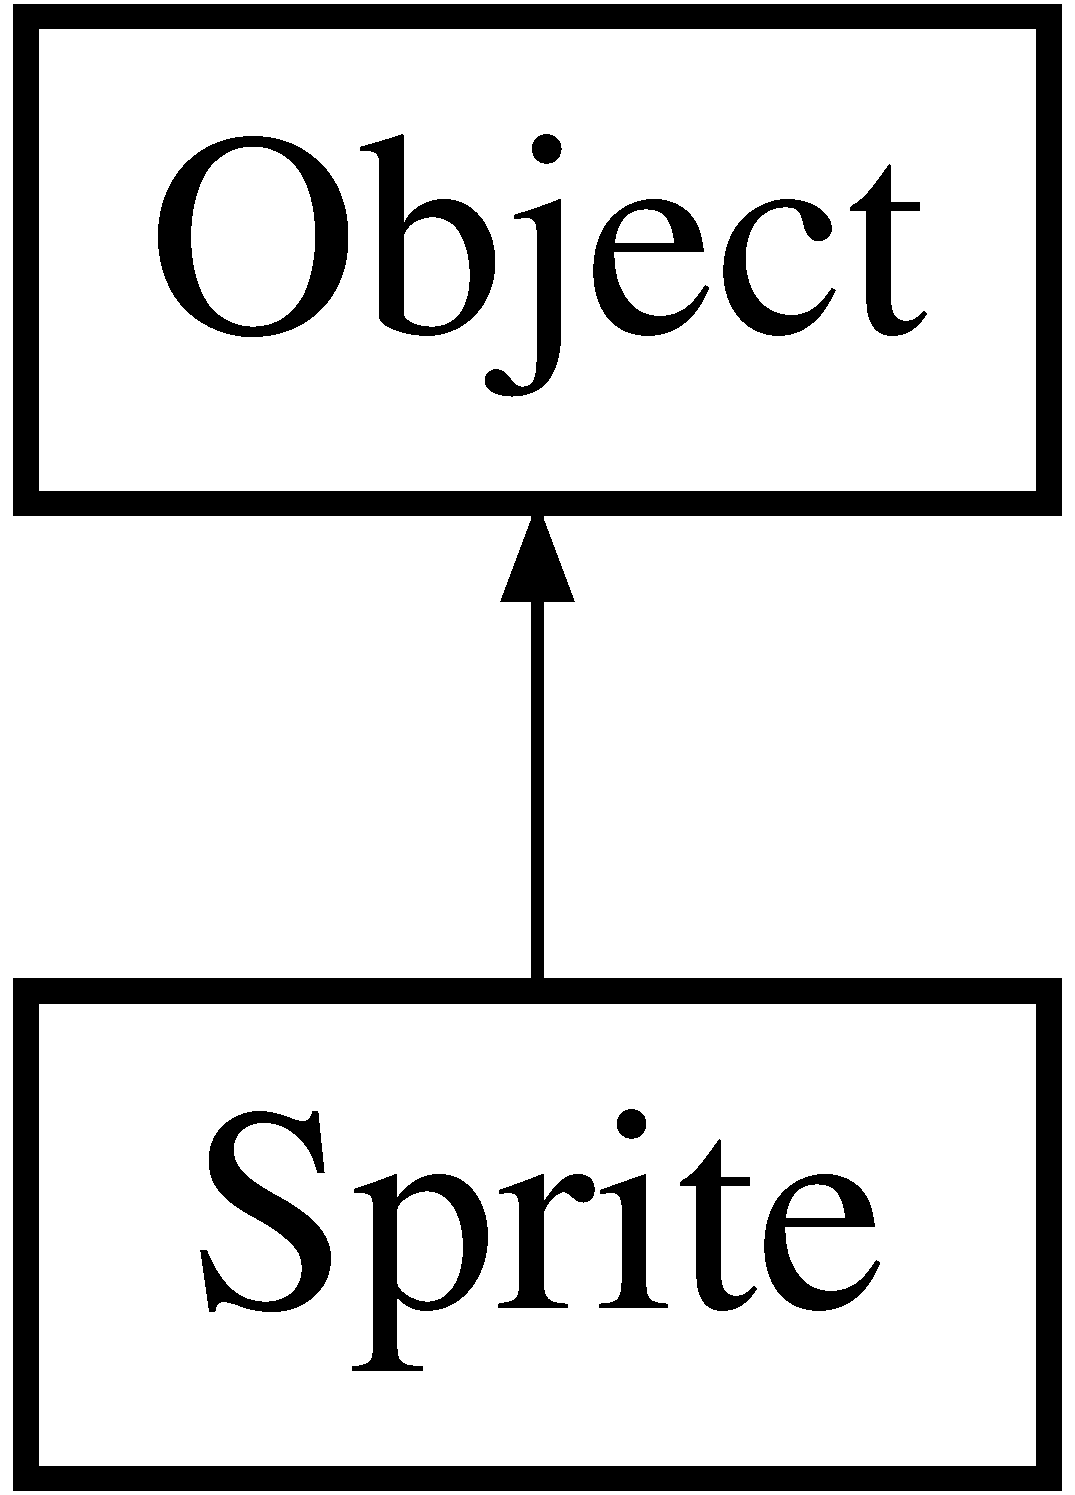
\includegraphics[height=2.000000cm]{class_sprite}
\end{center}
\end{figure}
\subsection*{Public Member Functions}
\begin{DoxyCompactItemize}
\item 
\hyperlink{class_sprite_a12cba3ac1868418add3c4d95ce87e615}{Sprite} ()
\item 
\hyperlink{class_sprite_a28604acdc189d2f99b4525e2fa12a585}{Sprite} (std\-::string file\-Name)
\item 
\hyperlink{class_sprite_a8accab430f9d90ae5117b57d67e32b84}{$\sim$\-Sprite} ()
\item 
void \hyperlink{class_sprite_a0d00170fb8cc22361e2c16c4b3818e7e}{draw} (float x, float y, float w, float h, std\-::string param=\char`\"{}\char`\"{})
\item 
void \hyperlink{class_sprite_a3689496f6c44c2c6fd9dd6bd92bf1742}{bind} ()
\end{DoxyCompactItemize}


\subsection{Detailed Description}
Class for handle single drawable objects. 

\subsection{Constructor \& Destructor Documentation}
\hypertarget{class_sprite_a12cba3ac1868418add3c4d95ce87e615}{\index{Sprite@{Sprite}!Sprite@{Sprite}}
\index{Sprite@{Sprite}!Sprite@{Sprite}}
\subsubsection[{Sprite}]{\setlength{\rightskip}{0pt plus 5cm}Sprite\-::\-Sprite (
\begin{DoxyParamCaption}
{}
\end{DoxyParamCaption}
)\hspace{0.3cm}{\ttfamily [inline]}}}\label{class_sprite_a12cba3ac1868418add3c4d95ce87e615}
Default constructor \hypertarget{class_sprite_a28604acdc189d2f99b4525e2fa12a585}{\index{Sprite@{Sprite}!Sprite@{Sprite}}
\index{Sprite@{Sprite}!Sprite@{Sprite}}
\subsubsection[{Sprite}]{\setlength{\rightskip}{0pt plus 5cm}Sprite\-::\-Sprite (
\begin{DoxyParamCaption}
\item[{std\-::string}]{file\-Name}
\end{DoxyParamCaption}
)\hspace{0.3cm}{\ttfamily [inline]}}}\label{class_sprite_a28604acdc189d2f99b4525e2fa12a585}
Constructor 
\begin{DoxyParams}{Parameters}
{\em file\-Name} & name of graphic file (.png) \\
\hline
\end{DoxyParams}
\hypertarget{class_sprite_a8accab430f9d90ae5117b57d67e32b84}{\index{Sprite@{Sprite}!$\sim$\-Sprite@{$\sim$\-Sprite}}
\index{$\sim$\-Sprite@{$\sim$\-Sprite}!Sprite@{Sprite}}
\subsubsection[{$\sim$\-Sprite}]{\setlength{\rightskip}{0pt plus 5cm}Sprite\-::$\sim$\-Sprite (
\begin{DoxyParamCaption}
{}
\end{DoxyParamCaption}
)}}\label{class_sprite_a8accab430f9d90ae5117b57d67e32b84}
Destructor, free memory 

\subsection{Member Function Documentation}
\hypertarget{class_sprite_a3689496f6c44c2c6fd9dd6bd92bf1742}{\index{Sprite@{Sprite}!bind@{bind}}
\index{bind@{bind}!Sprite@{Sprite}}
\subsubsection[{bind}]{\setlength{\rightskip}{0pt plus 5cm}void Sprite\-::bind (
\begin{DoxyParamCaption}
{}
\end{DoxyParamCaption}
)\hspace{0.3cm}{\ttfamily [inline]}, {\ttfamily [virtual]}}}\label{class_sprite_a3689496f6c44c2c6fd9dd6bd92bf1742}
Bind graphic for drawing 

Reimplemented from \hyperlink{class_object_a210c8bac4e5705ffee71d0837e46ab46}{Object}.

\hypertarget{class_sprite_a0d00170fb8cc22361e2c16c4b3818e7e}{\index{Sprite@{Sprite}!draw@{draw}}
\index{draw@{draw}!Sprite@{Sprite}}
\subsubsection[{draw}]{\setlength{\rightskip}{0pt plus 5cm}void Sprite\-::draw (
\begin{DoxyParamCaption}
\item[{float}]{x, }
\item[{float}]{y, }
\item[{float}]{w, }
\item[{float}]{h, }
\item[{std\-::string}]{param = {\ttfamily \char`\"{}\char`\"{}}}
\end{DoxyParamCaption}
)\hspace{0.3cm}{\ttfamily [virtual]}}}\label{class_sprite_a0d00170fb8cc22361e2c16c4b3818e7e}
Draw sprite on screen 
\begin{DoxyParams}{Parameters}
{\em x} & coordinate \\
\hline
{\em y} & coordinate \\
\hline
{\em w} & width \\
\hline
{\em h} & height \\
\hline
{\em param} & full draw string \\
\hline
\end{DoxyParams}


Reimplemented from \hyperlink{class_object_a13b99ec4da0a1c798104560c492c2a7e}{Object}.



The documentation for this class was generated from the following files\-:\begin{DoxyCompactItemize}
\item 
view/sprite.\-h\item 
view/sprite.\-cpp\end{DoxyCompactItemize}

\hypertarget{class_text}{\section{Text Class Reference}
\label{class_text}\index{Text@{Text}}
}


{\ttfamily \#include $<$text.\-h$>$}

Inheritance diagram for Text\-:\begin{figure}[H]
\begin{center}
\leavevmode
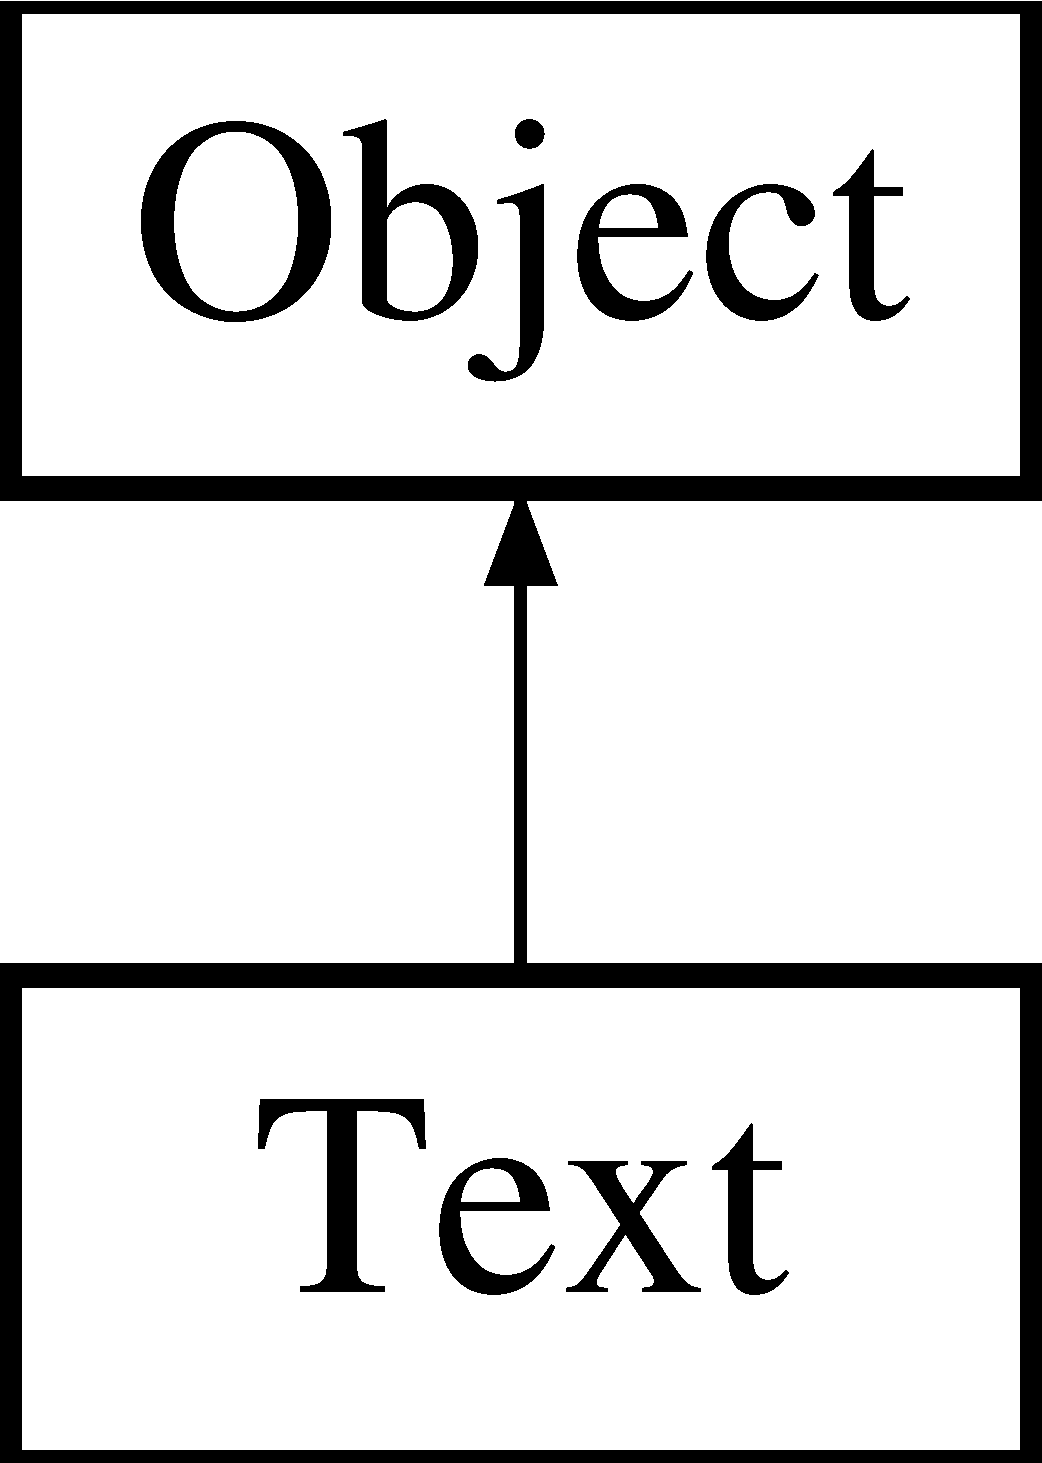
\includegraphics[height=2.000000cm]{class_text}
\end{center}
\end{figure}
\subsection*{Public Member Functions}
\begin{DoxyCompactItemize}
\item 
\hyperlink{class_text_ab3e26143fccc52699bcc5149cae852bc}{Text} ()
\item 
\hyperlink{class_text_ae78dd646ae9f0380530e4b1e39da7212}{Text} (std\-::string file\-Name, std\-::map$<$ std\-::string, \hyperlink{class_object}{Object} $\ast$ $>$ $\ast$igraphs)
\item 
void \hyperlink{class_text_a7eb6b5f04d40c5f3f482413612d0a101}{draw} (float x, float y, float w, float h, std\-::string param)
\end{DoxyCompactItemize}


\subsection{Detailed Description}
Class for text handling using \hyperlink{class_multi}{Multi} class 

\subsection{Constructor \& Destructor Documentation}
\hypertarget{class_text_ab3e26143fccc52699bcc5149cae852bc}{\index{Text@{Text}!Text@{Text}}
\index{Text@{Text}!Text@{Text}}
\subsubsection[{Text}]{\setlength{\rightskip}{0pt plus 5cm}Text\-::\-Text (
\begin{DoxyParamCaption}
{}
\end{DoxyParamCaption}
)\hspace{0.3cm}{\ttfamily [inline]}}}\label{class_text_ab3e26143fccc52699bcc5149cae852bc}
Default constructor \hypertarget{class_text_ae78dd646ae9f0380530e4b1e39da7212}{\index{Text@{Text}!Text@{Text}}
\index{Text@{Text}!Text@{Text}}
\subsubsection[{Text}]{\setlength{\rightskip}{0pt plus 5cm}Text\-::\-Text (
\begin{DoxyParamCaption}
\item[{std\-::string}]{file\-Name, }
\item[{std\-::map$<$ std\-::string, {\bf Object} $\ast$ $>$ $\ast$}]{igraphs}
\end{DoxyParamCaption}
)\hspace{0.3cm}{\ttfamily [inline]}}}\label{class_text_ae78dd646ae9f0380530e4b1e39da7212}
Constructor, load resources 
\begin{DoxyParams}{Parameters}
{\em file\-Name} & name of txh file \\
\hline
{\em igraphs} & graphics from view class \\
\hline
\end{DoxyParams}


\subsection{Member Function Documentation}
\hypertarget{class_text_a7eb6b5f04d40c5f3f482413612d0a101}{\index{Text@{Text}!draw@{draw}}
\index{draw@{draw}!Text@{Text}}
\subsubsection[{draw}]{\setlength{\rightskip}{0pt plus 5cm}void Text\-::draw (
\begin{DoxyParamCaption}
\item[{float}]{x, }
\item[{float}]{y, }
\item[{float}]{w, }
\item[{float}]{h, }
\item[{std\-::string}]{param}
\end{DoxyParamCaption}
)\hspace{0.3cm}{\ttfamily [virtual]}}}\label{class_text_a7eb6b5f04d40c5f3f482413612d0a101}
Draw text (font.\-txh\-::my\-\_\-text) 

Reimplemented from \hyperlink{class_object_a13b99ec4da0a1c798104560c492c2a7e}{Object}.



The documentation for this class was generated from the following files\-:\begin{DoxyCompactItemize}
\item 
view/text.\-h\item 
view/text.\-cpp\end{DoxyCompactItemize}

\hypertarget{class_text_input}{\section{Text\-Input Class Reference}
\label{class_text_input}\index{Text\-Input@{Text\-Input}}
}


{\ttfamily \#include $<$textinput.\-h$>$}

\subsection*{Public Member Functions}
\begin{DoxyCompactItemize}
\item 
\hyperlink{class_text_input_a3fe900efe9d41bf3d5e5d6acb5ac59d9}{Text\-Input} (\hyperlink{class_view}{View} \&iview)
\item 
\hyperlink{class_text_input_aa10eb8c9c85a5ebb7812ee441909c9e6}{$\sim$\-Text\-Input} ()
\item 
bool \hyperlink{class_text_input_a029a5ab670c9358c5165213e0966b344}{main\-Loop} ()
\item 
std\-::string \hyperlink{class_text_input_a0c4c73e5fe82d9987e4ba301b5153d28}{get\-Input} () const 
\end{DoxyCompactItemize}


\subsection{Detailed Description}
Get text from keyboard (A\-S\-C\-I\-I only) 

\subsection{Constructor \& Destructor Documentation}
\hypertarget{class_text_input_a3fe900efe9d41bf3d5e5d6acb5ac59d9}{\index{Text\-Input@{Text\-Input}!Text\-Input@{Text\-Input}}
\index{Text\-Input@{Text\-Input}!TextInput@{Text\-Input}}
\subsubsection[{Text\-Input}]{\setlength{\rightskip}{0pt plus 5cm}Text\-Input\-::\-Text\-Input (
\begin{DoxyParamCaption}
\item[{{\bf View} \&}]{iview}
\end{DoxyParamCaption}
)\hspace{0.3cm}{\ttfamily [inline]}}}\label{class_text_input_a3fe900efe9d41bf3d5e5d6acb5ac59d9}
Constructor 
\begin{DoxyParams}{Parameters}
{\em iview} & \hyperlink{class_view}{View} class \\
\hline
\end{DoxyParams}
\hypertarget{class_text_input_aa10eb8c9c85a5ebb7812ee441909c9e6}{\index{Text\-Input@{Text\-Input}!$\sim$\-Text\-Input@{$\sim$\-Text\-Input}}
\index{$\sim$\-Text\-Input@{$\sim$\-Text\-Input}!TextInput@{Text\-Input}}
\subsubsection[{$\sim$\-Text\-Input}]{\setlength{\rightskip}{0pt plus 5cm}Text\-Input\-::$\sim$\-Text\-Input (
\begin{DoxyParamCaption}
{}
\end{DoxyParamCaption}
)\hspace{0.3cm}{\ttfamily [inline]}}}\label{class_text_input_aa10eb8c9c85a5ebb7812ee441909c9e6}
Desctructor 

\subsection{Member Function Documentation}
\hypertarget{class_text_input_a0c4c73e5fe82d9987e4ba301b5153d28}{\index{Text\-Input@{Text\-Input}!get\-Input@{get\-Input}}
\index{get\-Input@{get\-Input}!TextInput@{Text\-Input}}
\subsubsection[{get\-Input}]{\setlength{\rightskip}{0pt plus 5cm}std\-::string Text\-Input\-::get\-Input (
\begin{DoxyParamCaption}
{}
\end{DoxyParamCaption}
) const\hspace{0.3cm}{\ttfamily [inline]}}}\label{class_text_input_a0c4c73e5fe82d9987e4ba301b5153d28}
After main loop ended, get entered text \hypertarget{class_text_input_a029a5ab670c9358c5165213e0966b344}{\index{Text\-Input@{Text\-Input}!main\-Loop@{main\-Loop}}
\index{main\-Loop@{main\-Loop}!TextInput@{Text\-Input}}
\subsubsection[{main\-Loop}]{\setlength{\rightskip}{0pt plus 5cm}bool Text\-Input\-::main\-Loop (
\begin{DoxyParamCaption}
{}
\end{DoxyParamCaption}
)}}\label{class_text_input_a029a5ab670c9358c5165213e0966b344}
The main loop 

The documentation for this class was generated from the following files\-:\begin{DoxyCompactItemize}
\item 
textinput.\-h\item 
textinput.\-cpp\end{DoxyCompactItemize}

\hypertarget{class_translate}{\section{Translate Class Reference}
\label{class_translate}\index{Translate@{Translate}}
}


{\ttfamily \#include $<$translate.\-h$>$}

\subsection*{Static Public Member Functions}
\begin{DoxyCompactItemize}
\item 
static \hyperlink{class_network_event}{Network\-Event} \hyperlink{class_translate_a7f99b4f8bc182e74931ba5b580de0842}{translate} (const char $\ast$buffer)
\item 
static void \hyperlink{class_translate_a251bfff8f099675f475fb96cbf629cbc}{translate} (std\-::vector$<$ \hyperlink{class_network_event}{Network\-Event} $>$ \&packets, const char $\ast$buffer, int bytes)
\item 
static void \hyperlink{class_translate_a5a0f76442c0c9a1ff0286109270b93da}{pack} (const \hyperlink{class_network_event}{Network\-Event} \&event, char $\ast$buffer)
\item 
static std\-::string \hyperlink{class_translate_a02e63cb5dbd8cc0759f5928cb2b435e4}{packet\-To\-String} (const char $\ast$buffer)
\item 
static char \hyperlink{class_translate_ab50f2648928eb66ded569f290afe1633}{slice} (char chr, bool first)
\end{DoxyCompactItemize}


\subsection{Detailed Description}
Static class, helper for network packet handling 

\subsection{Member Function Documentation}
\hypertarget{class_translate_a5a0f76442c0c9a1ff0286109270b93da}{\index{Translate@{Translate}!pack@{pack}}
\index{pack@{pack}!Translate@{Translate}}
\subsubsection[{pack}]{\setlength{\rightskip}{0pt plus 5cm}void Translate\-::pack (
\begin{DoxyParamCaption}
\item[{const {\bf Network\-Event} \&}]{event, }
\item[{char $\ast$}]{buffer}
\end{DoxyParamCaption}
)\hspace{0.3cm}{\ttfamily [static]}}}\label{class_translate_a5a0f76442c0c9a1ff0286109270b93da}
Make sendable packet from network event 
\begin{DoxyParams}{Parameters}
{\em event} & input \\
\hline
{\em buffer} & output \\
\hline
\end{DoxyParams}
\hypertarget{class_translate_a02e63cb5dbd8cc0759f5928cb2b435e4}{\index{Translate@{Translate}!packet\-To\-String@{packet\-To\-String}}
\index{packet\-To\-String@{packet\-To\-String}!Translate@{Translate}}
\subsubsection[{packet\-To\-String}]{\setlength{\rightskip}{0pt plus 5cm}std\-::string Translate\-::packet\-To\-String (
\begin{DoxyParamCaption}
\item[{const char $\ast$}]{buffer}
\end{DoxyParamCaption}
)\hspace{0.3cm}{\ttfamily [static]}}}\label{class_translate_a02e63cb5dbd8cc0759f5928cb2b435e4}
Packet to string, for trace \hypertarget{class_translate_ab50f2648928eb66ded569f290afe1633}{\index{Translate@{Translate}!slice@{slice}}
\index{slice@{slice}!Translate@{Translate}}
\subsubsection[{slice}]{\setlength{\rightskip}{0pt plus 5cm}char Translate\-::slice (
\begin{DoxyParamCaption}
\item[{char}]{chr, }
\item[{bool}]{first}
\end{DoxyParamCaption}
)\hspace{0.3cm}{\ttfamily [static]}}}\label{class_translate_ab50f2648928eb66ded569f290afe1633}
Split a char into two chars 
\begin{DoxyParams}{Parameters}
{\em chr} & input \\
\hline
{\em first} & lower of higher bytes \\
\hline
\end{DoxyParams}
\begin{DoxyReturn}{Returns}

\end{DoxyReturn}
\hypertarget{class_translate_a7f99b4f8bc182e74931ba5b580de0842}{\index{Translate@{Translate}!translate@{translate}}
\index{translate@{translate}!Translate@{Translate}}
\subsubsection[{translate}]{\setlength{\rightskip}{0pt plus 5cm}{\bf Network\-Event} Translate\-::translate (
\begin{DoxyParamCaption}
\item[{const char $\ast$}]{buffer}
\end{DoxyParamCaption}
)\hspace{0.3cm}{\ttfamily [static]}}}\label{class_translate_a7f99b4f8bc182e74931ba5b580de0842}
Make a single event from packet \hypertarget{class_translate_a251bfff8f099675f475fb96cbf629cbc}{\index{Translate@{Translate}!translate@{translate}}
\index{translate@{translate}!Translate@{Translate}}
\subsubsection[{translate}]{\setlength{\rightskip}{0pt plus 5cm}void Translate\-::translate (
\begin{DoxyParamCaption}
\item[{std\-::vector$<$ {\bf Network\-Event} $>$ \&}]{packets, }
\item[{const char $\ast$}]{buffer, }
\item[{int}]{bytes}
\end{DoxyParamCaption}
)\hspace{0.3cm}{\ttfamily [static]}}}\label{class_translate_a251bfff8f099675f475fb96cbf629cbc}
Make network events from packet received 
\begin{DoxyParams}{Parameters}
{\em packets} & output \\
\hline
{\em buffer} & input \\
\hline
{\em bytes} & input, number of bytes received \\
\hline
\end{DoxyParams}


The documentation for this class was generated from the following files\-:\begin{DoxyCompactItemize}
\item 
translate.\-h\item 
translate.\-cpp\end{DoxyCompactItemize}

\hypertarget{class_utf8}{\section{Utf8 Class Reference}
\label{class_utf8}\index{Utf8@{Utf8}}
}


{\ttfamily \#include $<$utf8.\-h$>$}

\subsection*{Public Member Functions}
\begin{DoxyCompactItemize}
\item 
\hyperlink{class_utf8_aea3f58e580b7fb3ed8f961aefdbb9248}{Utf8} ()
\item 
bool \hyperlink{class_utf8_a72c71cf43e8bf4db12dae3b95739c73e}{not\-Space} ()
\item 
bool \hyperlink{class_utf8_ada2987b0a3047f330a76318b3c99d0cc}{not\-Null} ()
\item 
bool \hyperlink{class_utf8_ac9c856a56d6f8f8487c95844f94c6b1f}{is\-Br} ()
\end{DoxyCompactItemize}
\subsection*{Friends}
\begin{DoxyCompactItemize}
\item 
std\-::ostream \& \hyperlink{class_utf8_adf7efdb1dd3c20c6c9fc763b1dadc444}{operator$<$$<$} (std\-::ostream \&output, const \hyperlink{class_utf8}{Utf8} \&u)
\item 
std\-::istream \& \hyperlink{class_utf8_ad15b5d0c4142ae3d72718db9bb3526b6}{operator$>$$>$} (std\-::istream \&input, \hyperlink{class_utf8}{Utf8} \&u)
\item 
bool \hyperlink{class_utf8_aad19f67bcbf91d10a9c94e713869ecbc}{operator==} (const \hyperlink{class_utf8}{Utf8} \&u, const \hyperlink{class_utf8}{Utf8} \&v)
\item 
bool \hyperlink{class_utf8_a55aa43861d5d089f5b48349219e515d3}{operator$>$} (const \hyperlink{class_utf8}{Utf8} \&u, const \hyperlink{class_utf8}{Utf8} \&v)
\item 
bool \hyperlink{class_utf8_ac2f8557ce9443a75715a990bb850f8c1}{operator$<$} (const \hyperlink{class_utf8}{Utf8} \&u, const \hyperlink{class_utf8}{Utf8} \&v)
\end{DoxyCompactItemize}


\subsection{Detailed Description}
Class for U\-T\-F-\/8 character handling 

\subsection{Constructor \& Destructor Documentation}
\hypertarget{class_utf8_aea3f58e580b7fb3ed8f961aefdbb9248}{\index{Utf8@{Utf8}!Utf8@{Utf8}}
\index{Utf8@{Utf8}!Utf8@{Utf8}}
\subsubsection[{Utf8}]{\setlength{\rightskip}{0pt plus 5cm}Utf8\-::\-Utf8 (
\begin{DoxyParamCaption}
{}
\end{DoxyParamCaption}
)\hspace{0.3cm}{\ttfamily [inline]}}}\label{class_utf8_aea3f58e580b7fb3ed8f961aefdbb9248}
Constructor 

\subsection{Member Function Documentation}
\hypertarget{class_utf8_ac9c856a56d6f8f8487c95844f94c6b1f}{\index{Utf8@{Utf8}!is\-Br@{is\-Br}}
\index{is\-Br@{is\-Br}!Utf8@{Utf8}}
\subsubsection[{is\-Br}]{\setlength{\rightskip}{0pt plus 5cm}bool Utf8\-::is\-Br (
\begin{DoxyParamCaption}
{}
\end{DoxyParamCaption}
)\hspace{0.3cm}{\ttfamily [inline]}}}\label{class_utf8_ac9c856a56d6f8f8487c95844f94c6b1f}
Character is not line-\/break \hypertarget{class_utf8_ada2987b0a3047f330a76318b3c99d0cc}{\index{Utf8@{Utf8}!not\-Null@{not\-Null}}
\index{not\-Null@{not\-Null}!Utf8@{Utf8}}
\subsubsection[{not\-Null}]{\setlength{\rightskip}{0pt plus 5cm}bool Utf8\-::not\-Null (
\begin{DoxyParamCaption}
{}
\end{DoxyParamCaption}
)\hspace{0.3cm}{\ttfamily [inline]}}}\label{class_utf8_ada2987b0a3047f330a76318b3c99d0cc}
Character is not null \hypertarget{class_utf8_a72c71cf43e8bf4db12dae3b95739c73e}{\index{Utf8@{Utf8}!not\-Space@{not\-Space}}
\index{not\-Space@{not\-Space}!Utf8@{Utf8}}
\subsubsection[{not\-Space}]{\setlength{\rightskip}{0pt plus 5cm}bool Utf8\-::not\-Space (
\begin{DoxyParamCaption}
{}
\end{DoxyParamCaption}
)\hspace{0.3cm}{\ttfamily [inline]}}}\label{class_utf8_a72c71cf43e8bf4db12dae3b95739c73e}
Character is not space 

\subsection{Friends And Related Function Documentation}
\hypertarget{class_utf8_ac2f8557ce9443a75715a990bb850f8c1}{\index{Utf8@{Utf8}!operator$<$@{operator$<$}}
\index{operator$<$@{operator$<$}!Utf8@{Utf8}}
\subsubsection[{operator$<$}]{\setlength{\rightskip}{0pt plus 5cm}bool operator$<$ (
\begin{DoxyParamCaption}
\item[{const {\bf Utf8} \&}]{u, }
\item[{const {\bf Utf8} \&}]{v}
\end{DoxyParamCaption}
)\hspace{0.3cm}{\ttfamily [friend]}}}\label{class_utf8_ac2f8557ce9443a75715a990bb850f8c1}
Less than operator \hypertarget{class_utf8_adf7efdb1dd3c20c6c9fc763b1dadc444}{\index{Utf8@{Utf8}!operator$<$$<$@{operator$<$$<$}}
\index{operator$<$$<$@{operator$<$$<$}!Utf8@{Utf8}}
\subsubsection[{operator$<$$<$}]{\setlength{\rightskip}{0pt plus 5cm}std\-::ostream\& operator$<$$<$ (
\begin{DoxyParamCaption}
\item[{std\-::ostream \&}]{output, }
\item[{const {\bf Utf8} \&}]{u}
\end{DoxyParamCaption}
)\hspace{0.3cm}{\ttfamily [friend]}}}\label{class_utf8_adf7efdb1dd3c20c6c9fc763b1dadc444}
Output operator, don't write second byte if it is null \begin{DoxyReturn}{Returns}
standard ostream 
\end{DoxyReturn}
\hypertarget{class_utf8_aad19f67bcbf91d10a9c94e713869ecbc}{\index{Utf8@{Utf8}!operator==@{operator==}}
\index{operator==@{operator==}!Utf8@{Utf8}}
\subsubsection[{operator==}]{\setlength{\rightskip}{0pt plus 5cm}bool operator== (
\begin{DoxyParamCaption}
\item[{const {\bf Utf8} \&}]{u, }
\item[{const {\bf Utf8} \&}]{v}
\end{DoxyParamCaption}
)\hspace{0.3cm}{\ttfamily [friend]}}}\label{class_utf8_aad19f67bcbf91d10a9c94e713869ecbc}
Equality operator \hypertarget{class_utf8_a55aa43861d5d089f5b48349219e515d3}{\index{Utf8@{Utf8}!operator$>$@{operator$>$}}
\index{operator$>$@{operator$>$}!Utf8@{Utf8}}
\subsubsection[{operator$>$}]{\setlength{\rightskip}{0pt plus 5cm}bool operator$>$ (
\begin{DoxyParamCaption}
\item[{const {\bf Utf8} \&}]{u, }
\item[{const {\bf Utf8} \&}]{v}
\end{DoxyParamCaption}
)\hspace{0.3cm}{\ttfamily [friend]}}}\label{class_utf8_a55aa43861d5d089f5b48349219e515d3}
Greater than operator \hypertarget{class_utf8_ad15b5d0c4142ae3d72718db9bb3526b6}{\index{Utf8@{Utf8}!operator$>$$>$@{operator$>$$>$}}
\index{operator$>$$>$@{operator$>$$>$}!Utf8@{Utf8}}
\subsubsection[{operator$>$$>$}]{\setlength{\rightskip}{0pt plus 5cm}std\-::istream\& operator$>$$>$ (
\begin{DoxyParamCaption}
\item[{std\-::istream \&}]{input, }
\item[{{\bf Utf8} \&}]{u}
\end{DoxyParamCaption}
)\hspace{0.3cm}{\ttfamily [friend]}}}\label{class_utf8_ad15b5d0c4142ae3d72718db9bb3526b6}
\hyperlink{class_input}{Input} operator, smartly determines U\-T\-F-\/8 characters and only read the second byte if it is valid U\-T\-F-\/8 character \begin{DoxyReturn}{Returns}
standard istream 
\end{DoxyReturn}


The documentation for this class was generated from the following file\-:\begin{DoxyCompactItemize}
\item 
view/utf8.\-h\end{DoxyCompactItemize}

\hypertarget{class_view}{\section{View Class Reference}
\label{class_view}\index{View@{View}}
}


{\ttfamily \#include $<$view.\-h$>$}

\subsection*{Public Member Functions}
\begin{DoxyCompactItemize}
\item 
\hyperlink{class_view_a44ad60a768422d3fa8fbd7576950080a}{View} ()
\item 
\hyperlink{class_view_ad0dc854db9aabbea98a334dec89f785c}{$\sim$\-View} ()
\item 
void \hyperlink{class_view_ac0b7ffdb316f54013052928c6e2e8ace}{swap} ()
\item 
bool \hyperlink{class_view_a2c7a00026247246c1f4b7b18b1cec20e}{load} (std\-::string file\-Name)
\item 
bool \hyperlink{class_view_a6edea19c9c4efd1a088d2ebbfbd3a240}{load\-Package} (std\-::string file\-Name)
\item 
void \hyperlink{class_view_a133f5487097d796a1b276f8c14f0671c}{draw} (\hyperlink{struct_rect}{Rect} r, std\-::string res)
\item 
void \hyperlink{class_view_a2a474840a5d346723e37dd01fd248e4e}{draw} (float x, float y, float w, float h, std\-::string res)
\item 
void \hyperlink{class_view_ab756d944d5d8a45c1ce6b365e6b6c27c}{resize\-\_\-event} (int \&w, int \&h)
\item 
void \hyperlink{class_view_a81b5809859fda85f39e0faa1b169e6d5}{draw\-Anim} ()
\item 
void \hyperlink{class_view_a067c5cbb6e248ae041c13d50da48d699}{stop\-Anim} ()
\item 
T\-I\-M\-E \hyperlink{class_view_a9cb2b63e68cff08050892f8d43909bf9}{get\-Now} ()
\item 
void \hyperlink{class_view_a33aeee3fb2659af067d1a279a2d96ed7}{set\-Now} ()
\item 
void \hyperlink{class_view_a51b9f1d6901753f868242ab9b3334dce}{set\-Tick\-Interval} (int i)
\item 
void \hyperlink{class_view_a2299069ba34803c1da65e0b43b6d7f10}{Screenshot} ()
\item 
void \hyperlink{class_view_a3f1c78cf35fbbed0019e9b835a118f19}{Toggle} ()
\item 
void \hyperlink{class_view_a62c7ef62ba7a4dab206a81ff999a2978}{frame\-Begin} ()
\item 
void \hyperlink{class_view_ac63fd1ddfcfb68d11f3a039ae8537765}{frame\-End} ()
\item 
T\-I\-M\-E \hyperlink{class_view_a911928e6ed1a440eafe321f2aab1c3e0}{frame\-Delay} ()
\end{DoxyCompactItemize}


\subsection{Detailed Description}
Main class for handling graphics 

\subsection{Constructor \& Destructor Documentation}
\hypertarget{class_view_a44ad60a768422d3fa8fbd7576950080a}{\index{View@{View}!View@{View}}
\index{View@{View}!View@{View}}
\subsubsection[{View}]{\setlength{\rightskip}{0pt plus 5cm}View\-::\-View (
\begin{DoxyParamCaption}
{}
\end{DoxyParamCaption}
)}}\label{class_view_a44ad60a768422d3fa8fbd7576950080a}
Constructor, initialize screen \hypertarget{class_view_ad0dc854db9aabbea98a334dec89f785c}{\index{View@{View}!$\sim$\-View@{$\sim$\-View}}
\index{$\sim$\-View@{$\sim$\-View}!View@{View}}
\subsubsection[{$\sim$\-View}]{\setlength{\rightskip}{0pt plus 5cm}View\-::$\sim$\-View (
\begin{DoxyParamCaption}
{}
\end{DoxyParamCaption}
)}}\label{class_view_ad0dc854db9aabbea98a334dec89f785c}
Destructor, unload objects 

\subsection{Member Function Documentation}
\hypertarget{class_view_a133f5487097d796a1b276f8c14f0671c}{\index{View@{View}!draw@{draw}}
\index{draw@{draw}!View@{View}}
\subsubsection[{draw}]{\setlength{\rightskip}{0pt plus 5cm}void View\-::draw (
\begin{DoxyParamCaption}
\item[{{\bf Rect}}]{r, }
\item[{std\-::string}]{res}
\end{DoxyParamCaption}
)}}\label{class_view_a133f5487097d796a1b276f8c14f0671c}
Draw on frame 
\begin{DoxyParams}{Parameters}
{\em r} & rectangle of drawing position \\
\hline
{\em res} & full drawing string \\
\hline
\end{DoxyParams}
\hypertarget{class_view_a2a474840a5d346723e37dd01fd248e4e}{\index{View@{View}!draw@{draw}}
\index{draw@{draw}!View@{View}}
\subsubsection[{draw}]{\setlength{\rightskip}{0pt plus 5cm}void View\-::draw (
\begin{DoxyParamCaption}
\item[{float}]{x, }
\item[{float}]{y, }
\item[{float}]{w, }
\item[{float}]{h, }
\item[{std\-::string}]{res}
\end{DoxyParamCaption}
)}}\label{class_view_a2a474840a5d346723e37dd01fd248e4e}
Draw on frame 
\begin{DoxyParams}{Parameters}
{\em x} & coordinate \\
\hline
{\em y} & coordinate \\
\hline
{\em w} & width \\
\hline
{\em h} & height \\
\hline
{\em res} & full drawing string \\
\hline
\end{DoxyParams}
\hypertarget{class_view_a81b5809859fda85f39e0faa1b169e6d5}{\index{View@{View}!draw\-Anim@{draw\-Anim}}
\index{draw\-Anim@{draw\-Anim}!View@{View}}
\subsubsection[{draw\-Anim}]{\setlength{\rightskip}{0pt plus 5cm}void View\-::draw\-Anim (
\begin{DoxyParamCaption}
{}
\end{DoxyParamCaption}
)}}\label{class_view_a81b5809859fda85f39e0faa1b169e6d5}
Draw animations on frame, delete ended animations \hypertarget{class_view_a62c7ef62ba7a4dab206a81ff999a2978}{\index{View@{View}!frame\-Begin@{frame\-Begin}}
\index{frame\-Begin@{frame\-Begin}!View@{View}}
\subsubsection[{frame\-Begin}]{\setlength{\rightskip}{0pt plus 5cm}void View\-::frame\-Begin (
\begin{DoxyParamCaption}
{}
\end{DoxyParamCaption}
)}}\label{class_view_a62c7ef62ba7a4dab206a81ff999a2978}
Begin of frame, actualilze time variables for current and previous frame \hypertarget{class_view_a911928e6ed1a440eafe321f2aab1c3e0}{\index{View@{View}!frame\-Delay@{frame\-Delay}}
\index{frame\-Delay@{frame\-Delay}!View@{View}}
\subsubsection[{frame\-Delay}]{\setlength{\rightskip}{0pt plus 5cm}T\-I\-M\-E View\-::frame\-Delay (
\begin{DoxyParamCaption}
{}
\end{DoxyParamCaption}
)}}\label{class_view_a911928e6ed1a440eafe321f2aab1c3e0}
Amount of sleep needed for enough frames per second \hypertarget{class_view_ac63fd1ddfcfb68d11f3a039ae8537765}{\index{View@{View}!frame\-End@{frame\-End}}
\index{frame\-End@{frame\-End}!View@{View}}
\subsubsection[{frame\-End}]{\setlength{\rightskip}{0pt plus 5cm}void View\-::frame\-End (
\begin{DoxyParamCaption}
{}
\end{DoxyParamCaption}
)}}\label{class_view_ac63fd1ddfcfb68d11f3a039ae8537765}
End of frame, sleep for a while to save C\-P\-U time \hypertarget{class_view_a9cb2b63e68cff08050892f8d43909bf9}{\index{View@{View}!get\-Now@{get\-Now}}
\index{get\-Now@{get\-Now}!View@{View}}
\subsubsection[{get\-Now}]{\setlength{\rightskip}{0pt plus 5cm}T\-I\-M\-E View\-::get\-Now (
\begin{DoxyParamCaption}
{}
\end{DoxyParamCaption}
)\hspace{0.3cm}{\ttfamily [inline]}}}\label{class_view_a9cb2b63e68cff08050892f8d43909bf9}
Get current frame time \hypertarget{class_view_a2c7a00026247246c1f4b7b18b1cec20e}{\index{View@{View}!load@{load}}
\index{load@{load}!View@{View}}
\subsubsection[{load}]{\setlength{\rightskip}{0pt plus 5cm}bool View\-::load (
\begin{DoxyParamCaption}
\item[{std\-::string}]{file\-Name}
\end{DoxyParamCaption}
)}}\label{class_view_a2c7a00026247246c1f4b7b18b1cec20e}
Load image, animation or text file 
\begin{DoxyParams}{Parameters}
{\em file\-Name} & name of file, extension determines the type \\
\hline
\end{DoxyParams}
\begin{DoxyReturn}{Returns}
success 
\end{DoxyReturn}
\hypertarget{class_view_a6edea19c9c4efd1a088d2ebbfbd3a240}{\index{View@{View}!load\-Package@{load\-Package}}
\index{load\-Package@{load\-Package}!View@{View}}
\subsubsection[{load\-Package}]{\setlength{\rightskip}{0pt plus 5cm}bool View\-::load\-Package (
\begin{DoxyParamCaption}
\item[{std\-::string}]{file\-Name}
\end{DoxyParamCaption}
)}}\label{class_view_a6edea19c9c4efd1a088d2ebbfbd3a240}
Load resources from list 
\begin{DoxyParams}{Parameters}
{\em file\-Name} & name of package \\
\hline
\end{DoxyParams}
\begin{DoxyReturn}{Returns}
success 
\end{DoxyReturn}
\hypertarget{class_view_ab756d944d5d8a45c1ce6b365e6b6c27c}{\index{View@{View}!resize\-\_\-event@{resize\-\_\-event}}
\index{resize\-\_\-event@{resize\-\_\-event}!View@{View}}
\subsubsection[{resize\-\_\-event}]{\setlength{\rightskip}{0pt plus 5cm}void View\-::resize\-\_\-event (
\begin{DoxyParamCaption}
\item[{int \&}]{w, }
\item[{int \&}]{h}
\end{DoxyParamCaption}
)}}\label{class_view_ab756d944d5d8a45c1ce6b365e6b6c27c}
Resize callback function 
\begin{DoxyParams}{Parameters}
{\em w} & width \\
\hline
{\em h} & height \\
\hline
\end{DoxyParams}
\hypertarget{class_view_a2299069ba34803c1da65e0b43b6d7f10}{\index{View@{View}!Screenshot@{Screenshot}}
\index{Screenshot@{Screenshot}!View@{View}}
\subsubsection[{Screenshot}]{\setlength{\rightskip}{0pt plus 5cm}void View\-::\-Screenshot (
\begin{DoxyParamCaption}
{}
\end{DoxyParamCaption}
)}}\label{class_view_a2299069ba34803c1da65e0b43b6d7f10}
Request to take screenshot at the end of frame \hypertarget{class_view_a33aeee3fb2659af067d1a279a2d96ed7}{\index{View@{View}!set\-Now@{set\-Now}}
\index{set\-Now@{set\-Now}!View@{View}}
\subsubsection[{set\-Now}]{\setlength{\rightskip}{0pt plus 5cm}void View\-::set\-Now (
\begin{DoxyParamCaption}
{}
\end{DoxyParamCaption}
)\hspace{0.3cm}{\ttfamily [inline]}}}\label{class_view_a33aeee3fb2659af067d1a279a2d96ed7}
Set current frame time to actual time \hypertarget{class_view_a51b9f1d6901753f868242ab9b3334dce}{\index{View@{View}!set\-Tick\-Interval@{set\-Tick\-Interval}}
\index{set\-Tick\-Interval@{set\-Tick\-Interval}!View@{View}}
\subsubsection[{set\-Tick\-Interval}]{\setlength{\rightskip}{0pt plus 5cm}void View\-::set\-Tick\-Interval (
\begin{DoxyParamCaption}
\item[{int}]{i}
\end{DoxyParamCaption}
)\hspace{0.3cm}{\ttfamily [inline]}}}\label{class_view_a51b9f1d6901753f868242ab9b3334dce}
Set refresh rate \hypertarget{class_view_a067c5cbb6e248ae041c13d50da48d699}{\index{View@{View}!stop\-Anim@{stop\-Anim}}
\index{stop\-Anim@{stop\-Anim}!View@{View}}
\subsubsection[{stop\-Anim}]{\setlength{\rightskip}{0pt plus 5cm}void View\-::stop\-Anim (
\begin{DoxyParamCaption}
{}
\end{DoxyParamCaption}
)}}\label{class_view_a067c5cbb6e248ae041c13d50da48d699}
Stop all animations \hypertarget{class_view_ac0b7ffdb316f54013052928c6e2e8ace}{\index{View@{View}!swap@{swap}}
\index{swap@{swap}!View@{View}}
\subsubsection[{swap}]{\setlength{\rightskip}{0pt plus 5cm}void View\-::swap (
\begin{DoxyParamCaption}
{}
\end{DoxyParamCaption}
)}}\label{class_view_ac0b7ffdb316f54013052928c6e2e8ace}
Swap buffers, draw on screen \hypertarget{class_view_a3f1c78cf35fbbed0019e9b835a118f19}{\index{View@{View}!Toggle@{Toggle}}
\index{Toggle@{Toggle}!View@{View}}
\subsubsection[{Toggle}]{\setlength{\rightskip}{0pt plus 5cm}void View\-::\-Toggle (
\begin{DoxyParamCaption}
{}
\end{DoxyParamCaption}
)\hspace{0.3cm}{\ttfamily [inline]}}}\label{class_view_a3f1c78cf35fbbed0019e9b835a118f19}
Request to toggle fullscreen 

The documentation for this class was generated from the following files\-:\begin{DoxyCompactItemize}
\item 
view/view.\-h\item 
view/view.\-cpp\end{DoxyCompactItemize}

%--- End generated contents ---

% Index
\newpage
\phantomsection
\addcontentsline{toc}{part}{Index}
\printindex

\end{document}
